\documentclass[11pt,a4paper]{article}
\usepackage[T1]{fontenc}
\usepackage[utf8]{inputenc}
\usepackage{lmodern}
\usepackage[margin=25mm,headheight=14pt]{geometry}
\usepackage{amsmath,amssymb,amsthm,mathtools}
\usepackage{booktabs,array,longtable}
\usepackage{graphicx,xcolor}
\usepackage{microtype}
\usepackage[round,authoryear]{natbib}
\usepackage{enumitem}
\usepackage{fancyhdr}
\usepackage{placeins,tocloft}
\setlength{\cftbeforesecskip}{3pt}
\setlength{\cftbeforepartskip}{8pt}
\definecolor{burgundy}{RGB}{113,28,45}
\definecolor{blue}{RGB}{28,74,112}
\usepackage[colorlinks=true,linkcolor=burgundy,citecolor=burgundy,urlcolor=blue]{hyperref}
\hypersetup{pdftitle={The Mathematics of Quantum Computing Advantage},
pdfauthor={Miquel Noguer i Alonso},
pdfsubject={Foundations, measurement, and operational cost frontiers},
pdfkeywords={quantum computing, quantum advantage, Shor, Grover, amplitude estimation}}
\pagestyle{fancy}
\fancyhf{}
\fancyhead[L]{\small Quantum Computing Advantage}
\fancyhead[R]{\small 15 November 2026}
\fancyfoot[C]{\thepage}
\setlength{\parskip}{4pt}
\setlength{\parindent}{0pt}
\setlength{\emergencystretch}{2em}
\setlist{itemsep=2pt,topsep=4pt}
\newcommand{\ket}[1]{\lvert #1\rangle}
\newcommand{\bra}[1]{\langle #1\rvert}
\newcommand{\braket}[2]{\langle #1\mid #2\rangle}
\newcommand{\norm}[1]{\left\lVert #1\right\rVert}
\newcommand{\abs}[1]{\left\lvert #1\right\rvert}
\newcommand{\E}{\mathbb E}
\newcommand{\C}{\mathbb C}
\newcommand{\R}{\mathbb R}
\newcommand{\F}{\mathbb F}
\newcommand{\Tr}{\operatorname{Tr}}
\newcommand{\poly}{\operatorname{poly}}
\newcommand{\diag}{\operatorname{diag}}
\newcommand{\rank}{\operatorname{rank}}
\newcommand{\Var}{\operatorname{Var}}
\newcommand{\TV}{d_{\mathrm{TV}}}
\newcommand{\BPP}{\mathsf{BPP}}
\newcommand{\BQP}{\mathsf{BQP}}
\newcommand{\PP}{\mathsf{PP}}
\newcommand{\NP}{\mathsf{NP}}
\newcommand{\PSPACE}{\mathsf{PSPACE}}
\newcommand{\reff}{r_{\mathrm{eff}}}
\newcommand{\rord}{r_{\mathrm{ord}}}
\newcommand{\nT}{m_{\mathrm{T}}}
\DeclareMathOperator{\gcdop}{gcd}
\newtheorem{theorem}{Theorem}[section]
\newtheorem{proposition}[theorem]{Proposition}
\newtheorem{lemma}[theorem]{Lemma}
\newtheorem{corollary}[theorem]{Corollary}
\theoremstyle{definition}
\newtheorem{definition}[theorem]{Definition}
\newtheorem{example}[theorem]{Example}
\theoremstyle{remark}
\newtheorem{remark}[theorem]{Remark}
\numberwithin{equation}{section}
\title{\textbf{The Mathematics of\\Quantum Computing Advantage}\\[6pt]
\large Foundations, measurement, and operational cost frontiers}
\author{Miquel Noguer i Alonso\\[-1pt]
\small Artificial Intelligence Finance Institute\\[-1pt]
\small\href{https://doi.org/10.5281/zenodo.24262887}{DOI: 10.5281/zenodo.24262887}}
\date{15 November 2026}
\begin{document}
\maketitle
\vspace{-15pt}
\begin{abstract}
When does a more expensive quantum measurement reduce the total cost of
distinguishing two known states? We study sequential experiments in which each
observation has a price and the experimenter can decide what to measure next
or when to stop. For a family of qubit experiments with two readouts, we
determine the smallest worst-case expected cost at each prescribed error
tolerance. Randomizing between at most two stopping thresholds attains this
cost. We characterize which pairs of qubit states realize the required
observation laws. For an explicit pair of full-rank, noncommuting states, the
second readout can carry a price premium of just under twenty percent and
still reduce total cost at sufficiently high confidence. At a premium of
twenty percent or more, the first readout alone is optimal at every confidence
level. Exact rational calculations and an independent dynamic programming
calculation certify these examples.

We then consider a calibrated binary phase oracle subject to dephasing. Each
experimental block incurs a fixed preparation cost and a cost proportional to
its depth. The experimenter can adapt the depth and measurement using earlier
outcomes, while retaining only classical information between blocks. We give
upper and lower bounds of the same order for the optimal expected cost. They
show how the phase separation, coherence time, and available circuit depth
jointly limit the useful duration of a block. In the noiseless model, we
determine the exact cost of discrimination with zero error. At high
confidence, measured relative entropy determines how much evidence a
measurement supplies per unit cost.

For finite catalogues of measurements and several competing hypotheses, we
show how finite decision programs approximate the minimax cost. An explicit
bound controls the error caused by truncating the experiment. When each
available measurement uniformly separates every pair of hypotheses, this error
decreases exponentially with the decision horizon.

\noindent\textbf{Keywords}\enspace Quantum state discrimination, sequential hypothesis testing, measurement cost, dephasing, optimal stopping, minimax decision theory.
\end{abstract}
\clearpage
\setcounter{tocdepth}{1}
{\small\setlength{\parskip}{0pt}\tableofcontents}
\clearpage
\section{Introduction: from quantum structure to decision cost}\label{sec:research}
A computational advantage compares experiments that produce the required
output at a prescribed cost and confidence. For a binary decision,
distinguishability per unit cost depends on both coherent evolution and
readout. Fixing one measurement can hide an improvement; treating a more
informative measurement as free can invent one.

\paragraph{Two levels of characterization.}
Theorem~\ref{thm:exact-price-frontier} solves the finite-confidence
minimax problem for a family of two readouts. A stopped-drift identity
and a likelihood-parity constraint give a converse attained by mixing
at most two integer barriers. Proposition~\ref{prop:lattice-realizability}
characterizes which qubit geometries realize that family.
Theorem~\ref{thm:sharp-price} gives an explicit noncommuting example with
sharp measurement-price threshold $6/5$; exact rational certificates
verify its full confidence--price frontier.
Theorem~\ref{thm:uniform-cost} addresses a different optimization: fresh
phase blocks with adaptive depth and arbitrary single-block POVMs. It
gives the uniform noise--depth--confidence law, with global multipliers
$1/70$ and $42$ and a factor-27 fixed-depth bracket
(Theorems~\ref{thm:sharp-global} and~\ref{thm:fixed-depth-sharp}).
Measured relative entropy supplies the exact high-confidence coefficient;
Theorem~\ref{thm:noiseless-converse} supplies the exact zero-error cost.
Theorem~\ref{thm:catalogue-exact} and
Corollary~\ref{cor:catalogue-exponential} extend the finite-confidence
characterization to priced finite catalogues through convergent policy
programs. Memory, calibration uncertainty, and utility-to-phase
comparisons are treated separately.

\paragraph{Scope.}
The closed-form phase law concerns a known binary phase family,
independently dephased blocks, affine expected cost, and classical
adaptation with no persistent quantum memory. The exact lattice frontier
optimizes over two declared readouts, not all POVMs. The catalogue results
allow arbitrary finite dimension and multiple hypotheses but retain a
finite menu of known observation laws. Collective measurements within
blocks have their own memory and entry costs. All sampling comparisons
use specified oracle interfaces; the numerical examples are mathematical
experiments, not hardware timings or unrestricted classical lower bounds.

\paragraph{Relation to prior work.}
Sequential likelihood-ratio testing and information-per-cost design are
classical \citep{wald1945,chernoff1959,nitinawarat2015}. Quantum sequential
testing establishes finite-mean perfect discrimination for pure states
\citep{vargas2021} and adaptive measured-relative-entropy rates
\citep{li2022}. The variational and projective-measurement reductions are
due to \citet{berta2017}. LP duality for sequential tests
\citep[Theorems 4.1--4.2]{fauss2015}, controlled sensor selection
\citep[Theorems 1--3]{lisensor2019}, and experiment simulation
\citep{blackwell1953} are established foundations, not new principles
claimed here. The specific developments are the uniform phase law, the
parity-based exactly solvable readout family, its quantum realizability
region and sharp price boundary, and explicit finite-cost certificates.
Related depth--query, noise, metrology, and resource-accounting work
includes \citet{giurgica2022,tanaka2021,demkowicz2012,dalzell2025}; composite
sequential quantum testing has separate asymptotic theory
\citep{simpson2026}. The present constructions do not claim a new general
computational-complexity separation or priority over all sequential-design
results.

Parts~\ref{part:foundations}--\ref{part:algorithms} develop the foundations
and algorithmic mechanisms. Part~\ref{part:operational} gives the costed
decision theory; the appendices treat utility margins, perturbations,
and workloads. No companion text is required.

\clearpage
\part{Quantum experiments and statistical information}\label{part:foundations}
\section{What must be compared?}\label{sec:comparison}
Let a task be specified by
\begin{equation}
 \mathcal T=(\mathcal I,\mathcal X_{\mathrm{acc}},\mathcal O,\varepsilon,\delta),
\end{equation}
where $\mathcal I$ is the input family, $\mathcal X_{\mathrm{acc}}$ is the allowed input-access
model, $\mathcal O$ is the required output, $\varepsilon$ is its error
tolerance, and $\delta$ is the allowed failure probability. Classical and
quantum algorithms must be compared on the same task, with their access
assumptions stated.

For example, returning all $N$ coordinates of a vector is different from
preparing a state whose amplitudes encode that vector. Estimating one
expectation is different from constructing a full probability table. Counting
calls to an oracle is different from timing its implementation.

\begin{definition}[Three meanings of advantage]
A \emph{query advantage} compares calls to specified black boxes.
A \emph{computational advantage} includes gate operations and classical
processing under a uniform computational model.
A \emph{practical advantage} compares total resources on specified
implementations, including preparation, error control, and readout.
\end{definition}

A useful accounting identity is
\begin{equation}\label{eq:ledger}
 T_Q=T_{\mathrm{setup}}+
 R\bigl(T_{\mathrm{prepare}}+T_{\mathrm{coherent}}+
 T_{\mathrm{measure}}\bigr)+T_{\mathrm{classical}},
\end{equation}
where $R$ is the number of executions. The terms must be defined to avoid
double counting: if a coherent routine repeatedly calls preparation and its
inverse, those calls belong inside $T_{\mathrm{coherent}}$.

A result $Q_Q=O(\sqrt{Q_C})$ about oracle calls does not imply
$T_Q=O(\sqrt{T_C})$ for elapsed time. A slower quantum oracle, an expensive
encoding, or many required observables can remove the gain.

\begin{example}[Input size versus numerical magnitude]
An integer $N$ has input length $n=\lfloor\log_2N\rfloor+1$. A cost $N^{1/2}$
is exponential in $n$, while a cost $n^3$ is polynomial in $n$. Every
speedup statement must specify which parameter grows.
\end{example}

\section{The mathematical space of a quantum computation}\label{sec:state}
\subsection{Tensor products, amplitudes, and projective geometry}
A qubit is a unit vector in $\C^2$:
\begin{equation}
 \ket{\psi}=\alpha\ket{0}+\beta\ket{1},\qquad
 |\alpha|^2+|\beta|^2=1.
\end{equation}
For $n$ qubits,
\begin{equation}\label{eq:hilbert}
 \mathcal H_n=(\C^2)^{\otimes n}\cong\C^{2^n},\qquad
 \ket{\psi}=\sum_{x\in\{0,1\}^n}\alpha_x\ket{x},\quad
 \sum_x|\alpha_x|^2=1.
\end{equation}
The Hilbert-space dimension is $2^n$. Normalization removes one real degree
of freedom, and the physically irrelevant global phase removes another.
Thus pure physical states form complex projective space
\begin{equation}
 \mathbb{CP}^{\,2^n-1},\qquad
 \dim_{\R}\mathbb{CP}^{\,2^n-1}=2^{n+1}-2.
\end{equation}
The geometry alone does not explain computational advantage. The state space is exponentially large, but the algorithm must
reach the relevant states using a short circuit and extract a useful answer
from them.

A classical probability distribution on $n$ bits also has $2^n$ entries.
Exponential description length is therefore not unique to quantum theory.
The operational distinction is the availability of complex amplitudes and
coherent transformations that combine them before taking squared moduli.

\subsection{Unitary dynamics and measurements}
An ideal closed-system computation applies a unitary matrix:
\begin{equation}
 \ket{\psi_{\mathrm{out}}}=U\ket{\psi_{\mathrm{in}}},\qquad U^\dagger U=I.
\end{equation}
A circuit is a factorization $U=U_L\cdots U_1$ into gates acting on a bounded
number of qubits. An arbitrary $2^n\times2^n$ unitary is not available at unit
cost. Generic unitaries require exponentially many parameters; efficient
algorithms use highly structured ones.

A measurement with positive operators $\{M_y\}$ satisfying $\sum_yM_y=I$
returns $y$ with probability
\begin{equation}\label{eq:born}
 p(y)=\bra{\psi}M_y\ket{\psi}.
\end{equation}
For computational-basis measurement, $M_y=\ket{y}\bra{y}$ and
$p(y)=|\alpha_y|^2$. One execution returns one outcome, not the amplitude
table.

For a Hermitian observable $O$, the mean measurement value is
\begin{equation}
 \langle O\rangle_\psi=\bra{\psi}O\ket{\psi}.
\end{equation}
Estimating this mean requires repeated preparation unless a stronger coherent
estimation procedure is available. If the measurement outcomes lie in
$[-1,1]$, ordinary independent measurements give additive error $\varepsilon$
with failure probability at most $\delta$ using
$O(\varepsilon^{-2}\log(1/\delta))$ executions.

\subsection{Mixed states and distinguishability}
Noise and partial information are represented by density matrices:
\begin{equation}
 \rho\succeq0,\quad \Tr\rho=1,\qquad p(y)=\Tr(M_y\rho).
\end{equation}
The trace distance
\begin{equation}
 D_{\mathrm{tr}}(\rho,\sigma)=\frac12\norm{\rho-\sigma}_1
\end{equation}
bounds the change in any measurement-event probability. For pure states,
\begin{equation}\label{eq:tracedistance}
 D_{\mathrm{tr}}(\ket{\psi}\bra{\psi},\ket{\phi}\bra{\phi})
 =\sqrt{1-|\braket{\psi}{\phi}|^2}
 \leq\norm{\ket{\psi}-\ket{\phi}}.
\end{equation}
This connects geometry to both error analysis and lower bounds: an algorithm
cannot reliably distinguish inputs whose final states remain too close.

\section{Channels, instruments, and the meaning of coherent access}
\label{sec:channels-foundations}
The passage from vectors to density operators is not merely a way to add
noise to an ideal circuit. It specifies which transformations remain
physical when a register is entangled with an unobserved reference.
Throughout this section all Hilbert spaces are finite-dimensional.

\subsection{Complete positivity and an environment representation}
A quantum channel $\Phi:\mathcal L(\mathcal H_A)\to
\mathcal L(\mathcal H_B)$ is linear, trace preserving, and completely
positive: $\Phi\otimes\operatorname{id}_R$ preserves positivity for
every reference space $\mathcal H_R$. Positivity on isolated inputs is
weaker. For example, transposition preserves eigenvalues, but partial
transposition of $\ket{\Omega}\bra{\Omega}$, with
$\ket{\Omega}=(\ket{00}+\ket{11})/\sqrt2$, has eigenvalues
$1/2,1/2,1/2,-1/2$. It cannot describe a physical local channel.

\begin{theorem}[Finite-dimensional channel representation]\label{thm:kraus-foundations}
A linear map is completely positive if and only if
\begin{equation}\label{eq:kraus-foundations}
 \Phi(A)=\sum_j K_j A K_j^\dagger.
\end{equation}
It is trace preserving exactly when $\sum_jK_j^\dagger K_j=I$.
In that case $V\ket{\psi}=\sum_jK_j\ket{\psi}\otimes\ket{j}$ is an
isometry and $\Phi(A)=\Tr_E(VAV^\dagger)$.
\end{theorem}
\begin{proof}
The forward representation is the finite-dimensional Choi theorem
\citep{choi1975}; its construction is short. Choose an orthonormal input
basis and form
$J_\Phi=\sum_{i,k}\ket{i}\bra{k}\otimes\Phi(\ket{i}\bra{k})$.
Complete positivity implies $J_\Phi\succeq0$, since it is the image
of the unnormalized maximally entangled projector under
$\operatorname{id}\otimes\Phi$. Write
$J_\Phi=\sum_j\ket{v_j}\bra{v_j}$ and define $K_j$ by
$\ket{v_j}=\sum_i\ket{i}\otimes K_j\ket{i}$.
Comparison of the $(i,k)$ blocks gives~\eqref{eq:kraus-foundations}.
Conversely, each term preserves positivity after tensoring with any
identity. Cyclicity of trace gives the trace-preservation condition,
which also implies $V^\dagger V=I$. Partial trace gives the last formula.
\end{proof}

The environment description explains decoherence without invoking an
unobserved classical measurement. For an isometry satisfying
$V\ket{0}=\ket{0}\ket{e_0}$ and $V\ket{1}=\ket{1}\ket{e_1}$,
discarding the environment multiplies the input $01$ matrix entry by
$\braket{e_1}{e_0}$. Orthogonal environment states erase that coherence;
identical environment states preserve it. The qubit dephasing channel
with visibility $v\in[0,1]$ has the explicit form
\begin{equation}\label{eq:dephasing-foundations}
 \mathcal D_v(\rho)=\frac{1+v}{2}\rho+
                   \frac{1-v}{2}Z\rho Z.
\end{equation}
It maps a Bloch vector $(x,y,z)$ to $(vx,vy,z)$, and
$\mathcal D_v\mathcal D_w=\mathcal D_{vw}$. Taking $v=e^{-\gamma}$
therefore gives visibility $e^{-\gamma t}$ after $t$ commuting phase
queries, exactly as assumed in Part~\ref{part:operational}.

\subsection{Outcome probabilities and post-measurement states}
A POVM $\{E_y\}$ specifies probabilities, but not the state after an
outcome. An instrument consists of completely positive maps
$\mathcal M_y$ whose sum is trace preserving. Its effect is
$E_y=\mathcal M_y^*(I)$; thus
\[
 p(y)=\Tr\mathcal M_y(\rho)=\Tr(E_y\rho),\qquad
 \rho_y=\mathcal M_y(\rho)/p(y)
\]
when $p(y)>0$. Distinct instruments can have the same POVM and different
state disturbances. In a restarted experiment the quantum output is
discarded, so only the POVM probabilities remain relevant. In a protocol
with quantum memory, that simplification is unavailable.

Any POVM has a direct isometric implementation:
$W\ket{\psi}=\sum_y\sqrt{E_y}\ket{\psi}\otimes\ket{y}$, for which
$W^\dagger W=I$. Measuring the last register realizes its effects.
This establishes physical realizability in principle. It does not make
the synthesis of $W$ free; a cost model must decide how to price it.

The dual channel satisfies
$\Tr[B\Phi(A)]=\Tr[\Phi^*(B)A]$ and is positive and unital.
Thus $0\preceq E\preceq I$ implies
$0\preceq\Phi^*(E)\preceq I$. This simple observation is the basis
for the distinguishability contraction proved below.

\subsection{Coherent access is more than access to samples}
Three interfaces must be distinguished: samples from a distribution;
preparation of a specified quantum state; and reversible access to a
preparation unitary, its inverse, and required controlled versions.
Each can supply different algorithmic information. A state-preparation
channel that discards its environment need not supply a coherent inverse.
An unspecified physical unitary channel also has no observable global
phase, while a controlled unitary turns that phase into a relative phase.

\begin{lemma}[The phase ambiguity of controlled access]
An interface giving only the channel $\rho\mapsto U\rho U^\dagger$
cannot specify a transformation that outputs the controlled unitary
$\ket{0}\bra{0}\otimes I+\ket{1}\bra{1}\otimes U$ for every chosen matrix
representative $U$.
\end{lemma}
\begin{proof}
$U=I$ and $U=-I$ define the same input channel. Their requested
controlled channels act as $I$ and $Z$ on the control register and
are distinguishable on $\ket{+}$. A transformation of the supplied
channel cannot distinguish two identical inputs.
\end{proof}

This elementary obstruction addresses a phase-specific target. Stronger
no-control results for an unknown unitary are established by
\citet{araujo2014}. A known circuit decomposition or a specified physical
reference can provide the missing structure. The controlled oracle in
the worked decision experiment is therefore a stated interface
assumption, not a consequence of ordinary sampling access.

\section{Distinguishability, information, and the choice of loss}
\label{sec:statistical-foundations}
Quantum states do not have one universally optimal measurement. An
optimal readout depends on the loss function, the prior or worst-case
criterion, the number of observations, and whether later experiments may
depend on earlier outcomes.

\subsection{The operational meaning of trace distance}
\begin{theorem}[Binary minimum-error discrimination]\label{thm:helstrom-foundations}
For states $\rho,\sigma$ with priors $\pi,1-\pi$, the minimum average
error over all measurements and binary decisions is
\begin{equation}\label{eq:helstrom-foundations}
 e_\pi^*(\rho,\sigma)=
 \frac{1-\|\pi\rho-(1-\pi)\sigma\|_1}{2}.
\end{equation}
For equal priors this is $(1-D_{\rm tr}(\rho,\sigma))/2$.
\end{theorem}
\begin{proof}
Merge all outcomes deciding $\rho$ into an effect $E$, with
$0\preceq E\preceq I$. Its success probability is
$(1-\pi)+\Tr(E\Delta)$, where
$\Delta=\pi\rho-(1-\pi)\sigma$.
The spectral decomposition maximizes the trace by taking $E$ to be
the projector onto the positive eigenspace of $\Delta$.
Since $\Tr\Delta=2\pi-1$,
$\Tr\Delta_+=(\|\Delta\|_1+2\pi-1)/2$. Subtraction from one
gives~\eqref{eq:helstrom-foundations}, the binary quantum detection
formula \citep{helstrom1969}.
\end{proof}

For traceless Hermitian $A$, the same spectral argument gives
$\max_{0\preceq E\preceq I}|\Tr(EA)|=\|A\|_1/2$.
Consequently trace distance is the largest possible difference in
measurement-event probabilities. It is also the maximum total
variation distance over POVMs: group the outcomes with positive
probability difference into one effect.

\begin{corollary}[Processing cannot improve single-copy discrimination]
For every channel $\Phi$,
\begin{equation}
 D_{\rm tr}(\Phi(\rho),\Phi(\sigma))
 \leq D_{\rm tr}(\rho,\sigma).
\end{equation}
\end{corollary}
\begin{proof}
Pull any output effect back through the positive unital map $\Phi^*$.
It becomes an admissible input effect, so the supremum of its probability
difference cannot exceed the input supremum.
\end{proof}

\subsection{Pure-state overlap and deterministic sample budgets}
For two pure states choose phases so that their overlap is
$q\in[0,1]$. In their two-dimensional span, write
$\ket{\phi}=q\ket{\psi}+\sqrt{1-q^2}\ket{\psi^\perp}$.
The difference of their rank-one projectors has eigenvalues
$\pm\sqrt{1-q^2}$. This proves~\eqref{eq:tracedistance} and gives,
for $n$ independent copies and an arbitrary collective measurement,
\begin{equation}\label{eq:pure-fixed-budget}
 e_n^*=\frac{1-\sqrt{1-q^{2n}}}{2}.
\end{equation}
For $0<q<1$ and $0<\delta<1/2$, the condition $e_n^*\leq\delta$
is equivalent to
\[
 n\geq\frac{\log[1/(4\delta(1-\delta))]}{-2\log q}.
\]
Every finite deterministic copy budget has positive error. This does not
contradict a sequential zero-error protocol with finite mean cost:
its stopping time can have an unbounded tail. In the symmetric
unambiguous construction of Proposition~\ref{prop:usd},
$\Pr(N>n)=q^n$ and $\E N=(1-q)^{-1}$.
The distinction between expected and deterministic resources is therefore
mathematical, not terminological.

For a POVM on a pure-state pair, the classical affinity
$\sum_y\sqrt{p_yq_y}$ is at least the overlap $q$.
Indeed,
\[
 q=\left|\sum_y\bra{\psi} E_y\ket{\phi}\right|
 \leq\sum_y\sqrt{\bra{\psi} E_y\ket{\psi}\,
                        \bra{\phi} E_y\ket{\phi}}.
\]
Unlike relative entropy, this quantity remains finite at the pure-state
boundary. Its decrement, rather than a divergent KL rate, controls the
noiseless cost converse in Theorem~\ref{thm:noiseless-converse}.

\subsection{Relative entropy measures accumulated evidence}
For finite probability laws $p,q$ define
$D_{\rm KL}(p\|q)=\sum_y p_y\log(p_y/q_y)$, with the usual support
convention. It is the expected log-likelihood increment under $p$.
The opposite direction generally has a different value. Under a common
classical channel $K$, the log-sum inequality applied separately at each
output gives
\[
 D_{\rm KL}(pK\|qK)\leq D_{\rm KL}(p\|q).
\]
For product observations, independence makes their log likelihoods
additive. Sequential designs preserve this conditional additivity even
when the observation rule is selected from the preceding transcript.

The quantum relative entropy
$D(\rho\|\sigma)=\Tr\rho(\log\rho-\log\sigma)$ is finite only
when the support of $\rho$ is contained in that of $\sigma$.
The measured relative entropy is
\[
 D_M(\rho\|\sigma)=\sup_{\{E_y\}}
 D_{\rm KL}\bigl(\{\Tr\rho E_y\}\|\{\Tr\sigma E_y\}\bigr).
\]
This is the evidence accessible from one measured copy, whereas the
operator expression need not be attainable by a single-copy readout.
Part~\ref{part:operational} makes that distinction quantitative in a
two-state family. Trace distance optimizes immediate binary decision
error; relative entropy optimizes the long-run directed evidence rate.
The optimizers need not coincide.

\subsection{Accessible classical information is limited by dimension}
Let a classical label $X=x$ select state $\rho_x$ with probability $p_x$,
and put $\bar\rho=\sum_xp_x\rho_x$. For a measurement outcome $Y$,
the Holevo bound is
\begin{equation}\label{eq:holevo-foundations}
 I(X:Y)\leq\chi:=S(\bar\rho)-\sum_xp_xS(\rho_x)
 \leq\log d,\qquad S(\rho)=-\Tr\rho\log\rho,
\end{equation}
where $d$ is the transmitted system dimension \citep{holevo1973}.
One way to see the first inequality is to write
$I(X:Y)=\sum_xp_xD_{\rm KL}(p_{Y|x}\|p_Y)$, apply measurement
data processing to each term, and use
$\sum_xp_xD(\rho_x\|\bar\rho)=\chi$.
The last inequality follows from $0\leq S(\rho_x)$ and
$S(\bar\rho)\leq\log d$.
Thus an $n$-qubit system, without preshared entanglement or additional
side information, conveys at most $n$ bits of accessible classical
information per transmitted system. This limits readout; it does not
rule out computing a useful small output from a large structured input.

\section{Sequential experiments with an explicit resource price}
\label{sec:general-sequential}
The information-per-cost principle does not depend on a quantum circuit.
It becomes a quantum resource statement only after the action set and
observation laws have been derived from the permitted physical operations.

\subsection{A controlled experiment and its stopped likelihood}
Let $h\in\{+,-\}$. At step $j$ a protocol chooses action $a_j$ from
the classical history, pays $c(a_j)\geq c_{\min}>0$, and observes an
outcome with conditional law $p_{h,a_j}$. It may randomize using
hypothesis-independent coins and stop at $N$, with finite expected
cost under both hypotheses. Assume common support and a uniform bound
on $|\log(p_{+,a}(y)/p_{-,a}(y))|$.
Its log likelihood is
\begin{equation}\label{eq:general-loglikelihood}
 Z_N=\sum_{j=1}^N\log\frac{p_{+,a_j}(Y_j)}{p_{-,a_j}(Y_j)}.
\end{equation}
The action-selection and stopping kernels cancel in the likelihood
ratio because they are the same functions of the observed history
under either hypothesis. They can change what is observed but cannot
create evidence without observations.

Define the directed rate ceilings
\[
 J_+=\sup_a\frac{D_{\rm KL}(p_{+,a}\|p_{-,a})}{c(a)},\qquad
 J_-=\sup_a\frac{D_{\rm KL}(p_{-,a}\|p_{+,a})}{c(a)}.
\]
\begin{theorem}[A costed sequential testing converse]\label{thm:general-converse}
If both decision errors are at most $0<\delta<1/2$, then
\begin{equation}\label{eq:general-cost-converse}
 \max_h\E_h\sum_{j=1}^N c(a_j)
 \geq\max\left\{\frac{k_\delta}{J_+},
                \frac{k_\delta}{J_-}\right\},\qquad
 k_\delta=(1-2\delta)\log\frac{1-\delta}{\delta}.
\end{equation}
The convention $k_\delta/0=+\infty$ expresses impossibility when one
directed rate is zero.
\end{theorem}
\begin{proof}
Finite expected cost gives $\E_hN<\infty$. Bounded increments justify
the stopped likelihood identity and interchange of summation and
expectation. Under $h=+$,
\[
 D_{\rm KL}(P_+^{\rm stop}\|P_-^{\rm stop})
 =\E_+Z_N
 =\E_+\sum_{j=1}^N
      D_{\rm KL}(p_{+,a_j}\|p_{-,a_j})
 \leq J_+\E_+\sum_{j=1}^Nc(a_j).
\]
Coarsen the terminal transcript to the decision. If its errors are
$\alpha,\beta\leq\delta$, data processing gives the lower bound
$\operatorname{kl}(1-\alpha,\beta)\geq
\operatorname{kl}(1-\delta,\delta)=k_\delta$.
The minimization over this rectangle follows by differentiating binary
KL in its two arguments while $1-\alpha>\beta$.
Reverse the hypotheses to obtain the $J_-$ inequality.
\end{proof}

This is a costed version of the information argument underlying
sequential likelihood-ratio testing and controlled sensing
\citep{wald1945,chernoff1959,nitinawarat2015}. It is a converse, not an
automatic achievability theorem. If different actions maximize the two
directions, an adaptive controller must select the appropriate action
using incomplete information about the true hypothesis. Reflection
symmetry makes that issue tractable in Theorem~\ref{thm:measured}.

\subsection{Finite confidence, asymptotic rates, and resource frontiers}
An asymptotic statement $C_\delta/\log(1/\delta)\to1/J$ describes
the leading coefficient for fixed experiment parameters. It does not
remove overshoot, integer-depth choices, or the learning cost of selecting
an action at finite confidence. In particular, two methods may have
ordered limiting rates and still require a separate finite-confidence
comparison. The cost interval $[L_\delta,U_\delta]$ records both a
converse and an implementable protocol.

For methods $A,B$, the condition $U_A<L_B$ certifies that $A$ wins
throughout the corresponding minimax cost intervals. The condition
$L_A>U_B$ certifies that it loses. Overlapping intervals are unresolved
by those bounds; they are not evidence of equal cost. Multiplying only
one oracle price can change the ordering without changing either
algorithm's query complexity.

Suppose an action consumes a resource vector $v(a)\in\R_+^m$, including
preparation, queries, measurement, and classical processing. A positive
price vector $w$ yields $c_w(a)=w^\top v(a)$ and rate
$J(w)=\sup_a d(a)/(w^\top v(a))$. Changing $w$ explores different
resource tradeoffs; there is no implementation-independent conversion
from queries to elapsed time. A protocol dominated in every expected
resource coordinate cannot become optimal for a strictly positive price
vector. The affine price $c_0+c_1t$ below is a transparent two-resource
specialization of this general viewpoint.

The order of limits is equally substantive. Fixed positive noise and
$\delta\downarrow 0$ retain bounded single-block likelihood increments
and produce logarithmic confidence cost. At zero noise, disjoint support
of selected outcomes can make those increments infinite and permit
finite-mean exact discrimination. A uniform result must address both
mechanisms rather than substitute zero noise into a full-rank formula.


\FloatBarrier\clearpage
\part{Algorithmic mechanisms and their limits}\label{part:algorithms}
\section{Interference: computing before taking probabilities}\label{sec:interference}
\subsection{Why amplitudes are different from probabilities}
Suppose two computational paths contribute amplitudes $a$ and $b$ to the same
outcome. Its probability is
\begin{equation}\label{eq:interference}
 |a+b|^2=|a|^2+|b|^2+2\operatorname{Re}(a\overline b).
\end{equation}
The cross term can be positive or negative. Classical mutually exclusive
alternatives contribute nonnegative probabilities, without this cancellation.

For the Hadamard gate
\begin{equation}
 H=\frac1{\sqrt2}\begin{pmatrix}1&1\\1&-1\end{pmatrix},\qquad H^2=I,
\end{equation}
the state after one gate is $\ket{+}= (\ket{0}+\ket{1})/\sqrt2$. A second Hadamard
returns $\ket{0}$ exactly because the amplitude of $\ket{1}$ is
$(1-1)/2=0$. Measuring after the first gate destroys the coherence needed
for this deterministic return.

This cancellation is mathematically elementary. The algorithmic difficulty
is arranging it so that a desired global property survives while irrelevant
alternatives cancel.

\subsection{Phase kickback and Boolean Fourier analysis}
A reversible oracle for $f:\{0,1\}^n\to\{0,1\}$ acts as
\begin{equation}
 O_f\ket{x}\ket{b}=\ket{x}\ket{b\oplus f(x)}.
\end{equation}
Because $\ket{-}=(\ket{0}-\ket{1})/\sqrt2$ changes sign under a bit flip,
\begin{equation}\label{eq:kickback}
 O_f\ket{x}\ket{-}=(-1)^{f(x)}\ket{x}\ket{-}.
\end{equation}
Function values have become phases. Applying Hadamards before and after the
phase oracle gives
\begin{equation}\label{eq:fourierboolean}
 \ket{0^n}\longmapsto
 \sum_{y\in\{0,1\}^n}\widehat g(y)\ket{y},\qquad
 \widehat g(y)=2^{-n}\sum_x(-1)^{f(x)+x\cdot y},
\end{equation}
where $x\cdot y=\sum_i x_i y_i\pmod2$. Measurement samples squared Fourier
coefficients $|\widehat g(y)|^2$.

For the linear function $f(x)=s\cdot x$,
\begin{equation}
 \widehat g(y)=2^{-n}\sum_x(-1)^{x\cdot(s\oplus y)}
 =\mathbf1_{\{y=s\}}.
\end{equation}
One quantum query recovers all $n$ bits of $s$. Classically, $n$ queries
$f(e_i)$ suffice, and recovering a uniformly random $s$ with constant success
requires $\Omega(n)$ one-bit oracle answers. This is the
Bernstein--Vazirani mechanism \citep{bernstein1997}; it is a linear query separation, not an
exponential one.

The Deutsch--Jozsa promise asks whether $f$ is constant or balanced
\citep{deutsch1992}. The amplitude at
$y=0$ is then $\pm1$ or $0$. The resulting exact quantum test uses one query,
whereas exact deterministic classical testing can require $2^{n-1}+1$.
However, randomized classical sampling solves this promise with a constant
number of queries at constant error. This illustrates why the classical
comparison model matters.

\section{Simon's algorithm: a proved exponential query separation}\label{sec:simon}
\subsection{The promise and the Fourier constraint}
Let $f:\F_2^n\to\F_2^n$ satisfy, for an unknown nonzero $s$,
\begin{equation}\label{eq:simonpromise}
 f(x)=f(x')\quad\Longleftrightarrow\quad
 x'=x\ \text{or}\ x'=x\oplus s.
\end{equation}
The task is to recover $s$ through oracle access. Prepare
\begin{equation}
 2^{-n/2}\sum_x\ket{x}\ket{f(x)}.
\end{equation}
Conditioning on a measurement of the second register leaves the first in
\begin{equation}
 \frac{\ket{x_0}+\ket{x_0\oplus s}}{\sqrt2}.
\end{equation}
After $H^{\otimes n}$, the amplitude of $y$ is
\begin{equation}
 2^{-(n+1)/2}(-1)^{x_0\cdot y}
 \bigl(1+(-1)^{s\cdot y}\bigr).
\end{equation}
Consequently,
\begin{equation}\label{eq:simondist}
 \Pr(Y=y)=
 \begin{cases}
  2^{-(n-1)},&s\cdot y=0,\\
  0,&s\cdot y=1.
 \end{cases}
\end{equation}
Each query yields a uniformly random linear constraint on the hidden
string. The second-register measurement can also be omitted; tracing out
that register gives the same distribution on $Y$.

\begin{proposition}[Recovery probability]
With $m$ independent samples from \eqref{eq:simondist}, the probability that
their span fails to equal $s^\perp$ is less than $2^{n-1-m}$.
Thus $m=n-1+\lceil\log_2(1/\delta)\rceil$ samples suffice for failure
probability at most $\delta$.
\end{proposition}
\begin{proof}
The space $s^\perp$ has dimension $n-1$. If the samples do not span it, some
nonzero linear functional on this space vanishes on every sample.
Each such functional vanishes on a uniform sample with probability $1/2$.
There are $2^{n-1}-1$ nonzero functionals. The union bound gives
$(2^{n-1}-1)2^{-m}<2^{n-1-m}$. Gaussian elimination over $\F_2$ then finds
the one-dimensional nullspace, whose nonzero element is $s$.
\end{proof}

\subsection{Why classical queries need exponentially more information}
For the usual distribution in which $s$ and the distinct oracle labels are
random, a classical algorithm learns a useful equality only by querying
both members of a pair $\{x,x\oplus s\}$. Among $q$ queried inputs there are
at most $\binom{q}{2}$ candidate differences. Until a collision occurs, these
differences only rule out candidate secrets; the random labels supply no
additional structure.

For $q$ well below $2^{n/2}$, the collision probability is
$O(q^2/2^n)$, and exponentially many secrets remain consistent with a
collision-free transcript. This yields the bounded-error classical lower
bound $\Omega(2^{n/2})$. The matching scale follows from a birthday search.
The quantum algorithm needs $O(n)$ queries at fixed error \citep{simon1997}.

The exponential separation is \emph{proved in the oracle model}. It does not
by itself prove $\BPP\ne\BQP$ for ordinary explicitly described inputs.

\begin{example}[A three-bit hidden period]
For $s=101$, the allowed outcomes are
\begin{equation}
 s^\perp=\{000,010,101,111\},
\end{equation}
each with probability $1/4$. Observing $010$ and $101$ gives
$s_2=0$ and $s_1+s_3=0$, leaving the nonzero solution $s=101$.
The accompanying verification script constructs the full oracle circuit and checks this
distribution.
\end{example}

\section{Fourier transforms, phase estimation, and Shor's algorithm}\label{sec:shor}
\subsection{The quantum Fourier transform}
For $M=2^m$, define
\begin{equation}\label{eq:qft}
 F_M\ket{x}=\frac1{\sqrt M}\sum_{y=0}^{M-1}
 e^{2\pi ixy/M}\ket{y}.
\end{equation}
Its circuit uses $O(m^2)$ elementary Hadamard and controlled-phase gates
when those rotations are counted as elementary; compiling them into a
fixed finite gate set adds precision-dependent overhead.

A classical discrete Fourier transform on an explicitly supplied length-$M$
array takes $O(M\log M)$ arithmetic operations. This is not, by itself, a
fair exponential speedup claim: the quantum transform takes an encoded
state to another encoded state and does not print the $M$ transformed
coefficients.

\subsection{Phase estimation as a finite geometric sum}
Suppose $U\ket{u}=e^{2\pi i\phi}\ket{u}$, where $\phi\in[0,1)$.
Controlled powers $U^{2^j}$ produce
\begin{equation}
 \frac1{\sqrt M}\sum_{k=0}^{M-1}e^{2\pi ik\phi}\ket{k}\ket{u}.
\end{equation}
Applying $F_M^\dagger$ to the first register gives amplitude
\begin{align}
 a_y&=\frac1M\sum_{k=0}^{M-1}e^{2\pi ik(\phi-y/M)},\\
 \Pr(Y=y)&=\frac{\sin^2\!\bigl(\pi M(\phi-y/M)\bigr)}
 {M^2\sin^2\!\bigl(\pi(\phi-y/M)\bigr)},\label{eq:qpedist}
\end{align}
with limiting values used when numerator and denominator vanish.
If $M\phi$ is an integer, that integer is measured with certainty.

Let $y_\star$ be the closest grid point to $M\phi$, interpreted cyclically.
Then the circular phase error is at most $1/(2M)$ and
\begin{equation}
 \Pr(Y=y_\star)\geq \frac4{\pi^2}.
\end{equation}
Indeed, for $|\Delta|\leq1/(2M)$,
$\sin(\pi M|\Delta|)\geq2M|\Delta|$ and
$\sin(\pi|\Delta|)\leq\pi|\Delta|$, giving the bound directly.

The circuit has only $m$ controlled powers, but their implementation is
not generally free. If only controlled applications of $U$ and $U^\dagger$
are supplied as unit-cost queries, implementing these powers uses $M-1$
applications of $U$. Thus generic phase resolution $\varepsilon\sim M^{-1}$
costs $O(\varepsilon^{-1})$ queries, not $O(\log(1/\varepsilon))$.
Controlled access itself must be assumed or constructed; it is not
automatically available for an arbitrary unknown physical black box.

\subsection{Order finding}
For a composite integer $N$ and $a$ coprime to $N$, define its order
\begin{equation}
 {\rord}=\min\{k\geq1:a^k\equiv1\pmod N\}.
\end{equation}
The modular multiplication operator, suitably extended to a permutation on
the entire register, acts on the orbit of $\ket{1}$ by
\begin{equation}
 U_a\ket{a^k\bmod N}=\ket{a^{k+1}\bmod N}.
\end{equation}
Its orbit eigenstates are
\begin{equation}
 \ket{u_j}=\frac1{\sqrt {\rord}}\sum_{k=0}^{{\rord}-1}
 e^{-2\pi ijk/{\rord}}\ket{a^k\bmod N},\qquad
 U_a\ket{u_j}=e^{2\pi ij/{\rord}}\ket{u_j}.
\end{equation}
Since $\ket{1}={\rord}^{-1/2}\sum_j\ket{u_j}$, phase estimation samples
approximations to $j/{\rord}$ with a uniform latent $j$.

Choose a power of two $M$ such that $N^2\leq M<2N^2$. On a good
phase-estimation outcome,
\begin{equation}
 \left|\frac yM-\frac{j}{\rord}\right|\leq\frac1{2M}<\frac1{2{\rord}^2}.
\end{equation}
The reduced fraction associated with $j/{\rord}$ can then be recovered by
continued fractions. If $\gcdop(j,{\rord})=1$, its denominator is ${\rord}$.
Otherwise it is a divisor; repeat, combine information where appropriate,
and verify candidate orders by modular exponentiation.

Unlike generic powers of an unknown unitary, the powers of $U_a$ can be
implemented using modular multiplication by the classically precomputed
constants $a^{2^j}\bmod N$. Repeated squaring and reversible arithmetic make
the total cost polynomial in $\log N$.

\subsection{From an order to factors}
If ${\rord}$ is even, then
\begin{equation}
 (a^{{\rord}/2}-1)(a^{{\rord}/2}+1)\equiv0\pmod N.
\end{equation}
When $a^{{\rord}/2}\not\equiv-1\pmod N$, the greatest common divisors
\begin{equation}
 d_-=\gcdop(a^{{\rord}/2}-1,N),\qquad d_+=\gcdop(a^{{\rord}/2}+1,N)
\end{equation}
provide nontrivial factors. Standard preprocessing handles even integers
and perfect powers; random choices of $a$ and repetition give a randomized
polynomial-time factoring algorithm \citep{shor1997}.

For $N=15$ and $a=2$, ${\rord}=4$:
\begin{equation}
 2^4\equiv1\pmod{15},\quad
 \gcdop(2^2-1,15)=3,\quad \gcdop(2^2+1,15)=5.
\end{equation}
Using $M=256$, the ideal phase outcomes are $0,64,128,192$, each with
probability $1/4$. The outcomes $64$ and $192$ directly reveal denominator
$4$ after reduction.

The established theorem is polynomial-time quantum factoring. A
superpolynomial lower bound for all classical factoring algorithms is not
known. An exponential advantage claim for factoring is therefore not an
unconditional separation from every possible classical algorithm.

\section{Grover search: a two-dimensional rotation}\label{sec:grover}
\subsection{Deriving the amplification formula}
Suppose $K$ of $N$ items are marked, with $0<K<N$. Define normalized
superpositions of good and bad items, $\ket{G}$ and $\ket{B}$. The uniform state
is
\begin{equation}
 \ket{s}=\sin\theta\ket{G}+\cos\theta\ket{B},\qquad \sin^2\theta=\frac KN.
\end{equation}
Let the phase oracle be $S_G=I-2\Pi_G$ and the diffusion reflection be
$R_s=2\ket{s}\bra{s}-I$. Their product $Q=R_sS_G$, restricted to the ordered basis
$(\ket{G},\ket{B})$, is
\begin{equation}
 Q=\begin{pmatrix}\cos2\theta&\sin2\theta\\-\sin2\theta&\cos2\theta\end{pmatrix}.
\end{equation}
Repeated multiplication gives
\begin{equation}\label{eq:grover}
 Q^j\ket{s}=
 \sin((2j+1)\theta)\ket{G}+\cos((2j+1)\theta)\ket{B},\qquad
 P_j=\sin^2((2j+1)\theta).
\end{equation}
For small $K/N$, choose $j$ near $\pi/(4\theta)-1/2$. Then
\begin{equation}
 j=\Theta\!\left(\sqrt{\frac NK}\right),
\end{equation}
whereas classical unstructured search takes $\Theta(N/K)$ queries at
constant success probability. Unknown $K$ requires an adaptive or randomized
schedule rather than blindly choosing a fixed iteration count.

\begin{example}[One marked item among eight]
For $N=8$ and $K=1$, the first three success probabilities are
\begin{equation}
 P_0=\frac18,\qquad P_1=\frac{25}{32},\qquad
 P_2=\frac{121}{128}=0.9453125.
\end{equation}
At $j=3$, the probability decreases to $169/512=0.330078125$.
Amplification is coherent rotation, so continuing past the optimum can
undo the improvement.
\end{example}

\subsection{Why generic search cannot be exponentially accelerated}
The quadratic speedup is optimal in the black-box model
\citep{grover1996,bennett1997}. The following hybrid argument displays the
mechanism of the lower bound.

\begin{theorem}[An unstructured-search query lower bound]
Consider a quantum algorithm deciding whether a phase oracle marks no
item or exactly one of $N$ items, with error at most $1/3$ on every
promised input. If the algorithm uses $T$ oracle queries, then
$T\geq\sqrt N/6$.
\end{theorem}
\begin{proof}
Let $\ket{\psi_T^x}$ be its final state when $x$ is marked and
$\ket{\psi_T^\varnothing}$ its final state for the identity oracle.
Intermediate measurements can be deferred by adding work registers.
Let $p_t(x)$ be the query-register probability of $x$ just before query $t$
in the identity-oracle computation.

A telescoping replacement of the $T$ oracle calls and unitarity give
\begin{equation}
 \norm{\ket{\psi_T^x}-\ket{\psi_T^\varnothing}}
 \leq 2\sum_{t=1}^T\sqrt{p_t(x)}.
\end{equation}
Cauchy--Schwarz, followed by $\sum_xp_t(x)=1$, yields
\begin{equation}
 \sum_x\norm{\ket{\psi_T^x}-\ket{\psi_T^\varnothing}}^2
 \leq4T\sum_{t,x}p_t(x)=4T^2.
\end{equation}
The acceptance probability differs by at least $1/3$ between each marked
input and the unmarked input. Equation~\eqref{eq:tracedistance} therefore
implies that every summand is at least $1/9$. Hence $N/9\leq4T^2$.
\end{proof}

Searching all $2^n$ candidate solutions to a generic Boolean constraint
problem consequently takes order $2^{n/2}$ quantum queries in the
unstructured model. This remains exponential in $n$. The result does not
rule out faster algorithms exploiting special structure, and does not prove
a lower bound for all explicitly represented NP-complete problems.

\begin{figure}[t]
 \centering
 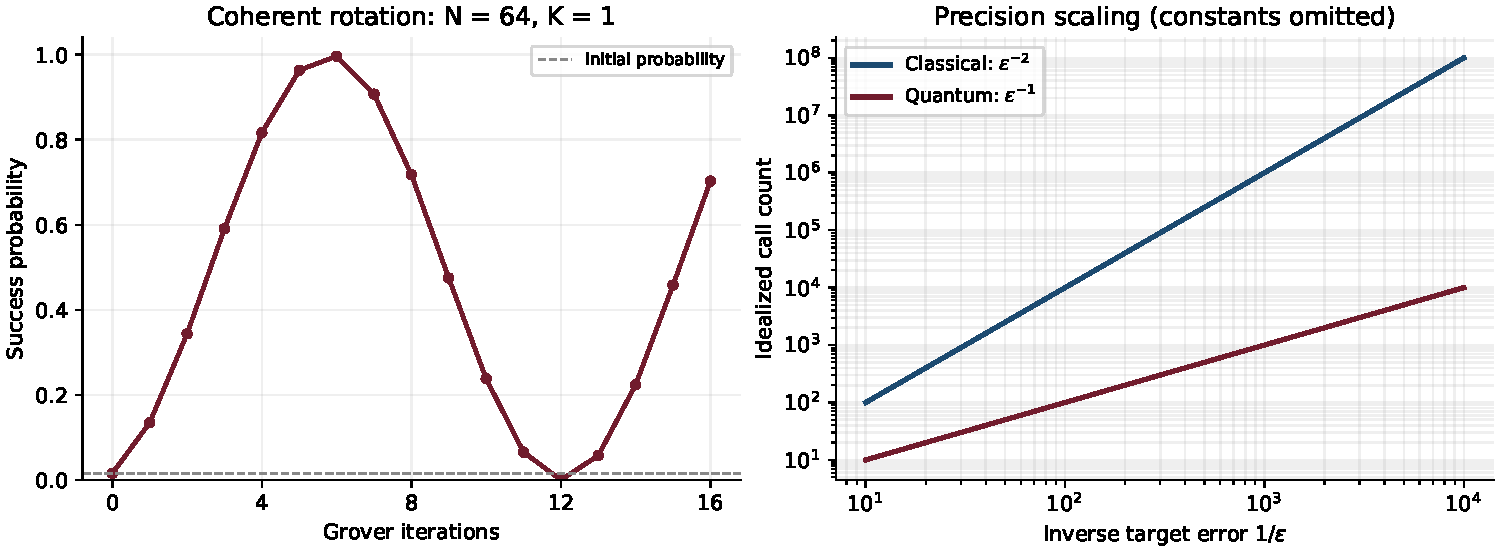
\includegraphics[width=\linewidth]{quantum_advantage_figures.pdf}
 \caption{Analytic illustrations, not hardware measurements.
 Left: the exact Grover success probability for one marked item among $64$.
 Right: idealized precision exponents for independent Monte Carlo samples
 and coherent amplitude estimation; constants and implementation costs
 are omitted.}
 \label{fig:scaling}
\end{figure}

\section{Amplitude estimation: an advantage in precision}\label{sec:amplitude}
\subsection{From an expectation to a probability amplitude}
Let $X$ take values in a finite set with probabilities $p_x$ and let
$0\leq f(x)\leq1$. Suppose a coherent circuit $U_{\mathrm{prep}}$ prepares
\begin{equation}\label{eq:expectationencoding}
 U_{\mathrm{prep}}\ket{0}=\sum_x\sqrt{p_x}\ket{x}
 \left(\sqrt{1-f(x)}\ket{0}+\sqrt{f(x)}\ket{1}\right).
\end{equation}
The probability that the final qubit is $1$ equals
\begin{equation}
 a=\sum_xp_x f(x)=\E[f(X)].
\end{equation}
We assume access to $U_{\mathrm{prep}}$, its inverse, the required controlled operations,
and reflections. A classical sampler that merely outputs independent values
of $X$ does not automatically provide these operations.

Ordinary sample means satisfy Hoeffding's bound
\begin{equation}
 \Pr(|\widehat a_m-a|>\varepsilon)\leq2e^{-2m\varepsilon^2}.
\end{equation}
Thus $m\geq \log(2/\delta)/(2\varepsilon^2)$ suffices. For Bernoulli means
bounded away from $0$ and $1$, $\Omega(\varepsilon^{-2})$ classical samples
are necessary at constant confidence: distinguishing parameters separated
by $O(\varepsilon)$ requires a constant statistical distance, while the
per-sample information is $O(\varepsilon^2)$.

\subsection{The rotation phase encodes the mean}
Write
\begin{equation}
 U_{\mathrm{prep}}\ket{0}=\sqrt a\ket{\Psi_1}+\sqrt{1-a}\ket{\Psi_0},\qquad a=\sin^2\theta.
\end{equation}
Reflections about $U_{\mathrm{prep}}\ket{0}$ and the good subspace yield the same
two-dimensional rotation as in Grover search. Its eigenvalues are
$e^{\pm2i\theta}$. Phase estimation therefore estimates $\theta$, from
which $a$ is recovered.

For a phase resolution parameter $M$, the canonical amplitude-estimation
guarantee is
\begin{equation}\label{eq:ae}
 |\widetilde a-a|
 \leq\frac{2\pi\sqrt{a(1-a)}}M+\frac{\pi^2}{M^2}
\end{equation}
with probability at least $8/\pi^2$, using $O(M)$ coherent oracle calls
\citep{brassard2002}. The functional dependence follows from
\begin{equation}
 \left|\sin^2(\theta+\Delta)-\sin^2\theta\right|
 \leq 2\sqrt{a(1-a)}|\Delta|+\Delta^2,
\end{equation}
obtained by Taylor's theorem and $|(\sin^2\theta)''|\leq2$.
Phase estimation supplies the corresponding $O(1/M)$ angular resolution.

Since $\sqrt{a(1-a)}\leq1/2$, the worst-case additive accuracy requires
$M=O(\varepsilon^{-1})$. Repeating independently and taking a median gives
\begin{equation}\label{eq:mcvsqae}
 Q_Q=O\!\left(\frac{\log(1/\delta)}{\varepsilon}\right),\qquad
 Q_C=O\!\left(\frac{\log(1/\delta)}{\varepsilon^2}\right).
\end{equation}
This is a quadratic precision advantage under coherent access. It is not an
exponential improvement in dimension. Generalizations to bounded-variance
random variables require additional constructions and qualifications
\citep{montanaro2015}.

\subsection{Absolute error, relative error, and total cost}
For a rare event of probability $a$, requiring relative error $\varepsilon_{\mathrm{rel}}$
means absolute error $\varepsilon=\varepsilon_{\mathrm{rel}} a$. The sharper bound
\eqref{eq:ae} suggests a query scale
$O(1/(\varepsilon_{\mathrm{rel}}\sqrt a))$ at constant confidence, while classical Bernoulli
sampling has scale $O(1/(\varepsilon_{\mathrm{rel}}^2a))$ for small $a$ and $\varepsilon_{\mathrm{rel}}$.
Using only the worst-case bound in \eqref{eq:mcvsqae} obscures this distinction.

Let a coherent call cost $c_Q$ and a classical sample cost $c_C$.
Suppressing confidence factors and constants, the comparison is
\begin{equation}
 T_Q\approx \frac{c_Q}{\varepsilon},\qquad
 T_C\approx \frac{c_C}{\varepsilon^2}.
\end{equation}
The quantum method wins in this simplified model only when
$\varepsilon\lesssim c_C/c_Q$. At $\varepsilon=10^{-3}$, the exponents
suggest $10^3$ versus $10^6$ calls; this is an illustration of scaling,
not a resource estimate.

For continuous inputs or unbounded payoffs, discretization, truncation, and
arithmetic also contribute:
\begin{equation}\label{eq:errorbudget}
 \begin{split}
 \varepsilon_{\mathrm{total}}\leq&
 \varepsilon_{\mathrm{model}}+\varepsilon_{\mathrm{discretization}}
 +\varepsilon_{\mathrm{truncation}}\\
 &+\varepsilon_{\mathrm{arithmetic}}+\varepsilon_{\mathrm{estimation}}.
 \end{split}
\end{equation}
Quantum computation can reduce the estimation cost without reducing the
other terms. The argument applies to scientific integration, reliability,
statistical physics, and financial expectations, subject to the same
access and error assumptions.

\section{Quantum simulation and the structure of operators}\label{sec:simulation}
\subsection{Local Hamiltonians avoid explicit exponential matrices}
A closed quantum system evolves according to
\begin{equation}
 i\frac{d}{dt}\ket{\psi(t)}=H\ket{\psi(t)},\qquad
 \ket{\psi(t)}=e^{-iHt}\ket{\psi(0)},
\end{equation}
using units with $\hbar=1$. For $n$ qubits, $H$ has dimension $2^n$, but
a local Hamiltonian may have a short description
\begin{equation}
 H=\sum_{\ell=1}^L H_\ell,
\end{equation}
where $L=\poly(n)$ and each $H_\ell$ acts on a fixed number of qubits.

For Hermitian terms, the first-order product formula obeys
\begin{equation}\label{eq:trotter}
 \left\|e^{-it\sum_\ell H_\ell}
 -\left(\prod_{\ell=1}^L e^{-iH_\ell t/{\nT}}\right)^{\nT}\right\|
 \leq \frac{t^2}{2{\nT}}\sum_{\ell<k}\norm{[H_\ell,H_k]}.
\end{equation}
Here the norm is the operator norm. A one-step integral remainder bounds
the error by $\Delta t^2\sum_{\ell<k}\|[H_\ell,H_k]\|/2$;
telescoping the ${\nT}\in\mathbb N$ unitary steps gives \eqref{eq:trotter}.
Commuting terms have zero error in this formula. More general commutator
analyses are developed by \citet{childs2021}.

This is a direct route to polynomial cost when the number and norms of terms,
evolution time, and inverse error are polynomially bounded and each local
exponential can be implemented efficiently. The task is to create the
evolved state and estimate specified observables. It is not to print all
$2^n$ amplitudes.

Quantum simulation is especially natural when the input and output are
already quantum. Nevertheless, easy classical subclasses exist, and a
generic classical hardness claim requires more than the matrix dimension.

\subsection{Block encoding and polynomial approximation}
Let $B$ be a matrix and $\alpha\geq\|B\|$. A unitary $U_B$ is an exact
block encoding if
\begin{equation}\label{eq:block}
 (\bra{0^a}\otimes I)U_B(\ket{0^a}\otimes I)=B/\alpha.
\end{equation}
It exposes a possibly nonunitary matrix as a block of a larger unitary.
The cost of constructing and querying $U_B$ is part of the input model.

Quantum singular value transformation (QSVT) uses alternating unitary
queries and phase rotations to implement polynomial transformations of
encoded singular values. The polynomial must obey boundedness and parity
conditions; it is not an arbitrary unbounded scalar function applied for
free. In a suitable exact encoding, a degree-$d$ admissible transformation
uses $O(d)$ queries \citep{gilyen2019}.

For a Hermitian contraction $H/\alpha$ with eigenvalue $\lambda/\alpha$,
qubitization produces an invariant two-dimensional subspace with eigenphases
$\pm\arccos(\lambda/\alpha)$. Polynomial approximation can then synthesize
$e^{-i\lambda t}$ across the spectral interval. A useful sufficient query
bound is
\begin{equation}
 O\!\left(\alpha|t|+\log(1/\varepsilon)\right)
\end{equation}
for the standard coherent access model, with refinements available
\citep{low2019}. This convenient sufficient bound is not the sharp
precision dependence. For fixed nonzero normalized evolution scale,
optimal query precision dependence is
$\Theta(\log(1/\varepsilon)/\log\log(1/\varepsilon))$ in the
corresponding black-box simulation model \citep{low2017}. This is a query bound, not a gate count for an arbitrary
dense Hamiltonian.

\subsection{An explicit two-dimensional spectral calculation}
The geometry can be seen without invoking a full circuit synthesis theorem.
For a Hermitian contraction $B$, the matrix
\begin{equation}
 U_B=\begin{pmatrix}
 B&\sqrt{I-B^2}\\
 \sqrt{I-B^2}&-B
 \end{pmatrix}
\end{equation}
is unitary because $B$ commutes with its spectral function
$\sqrt{I-B^2}$ and $U_B^2=I$. Multiplying by the reflection
$Z_a=\diag(I,-I)$ gives $W=Z_aU_B$. On an eigenvector of $B$
with eigenvalue $x\in[-1,1]$, it acts as
\begin{equation}
 W(x)=\begin{pmatrix}
 x&\sqrt{1-x^2}\\
 -\sqrt{1-x^2}&x
 \end{pmatrix},
 \qquad \operatorname{spec}W(x)=
 \{e^{i\arccos x},e^{-i\arccos x}\}.
\end{equation}
Consequently, the upper-left entry of $W(x)^d$ is
\begin{equation}
 T_d(x)=\cos(d\arccos x),
\end{equation}
the degree-$d$ Chebyshev polynomial. A sequence of rotations therefore
creates a polynomial transformation of an encoded eigenvalue. Phase choices
and ancillary constructions extend this principle to the admissible
polynomials used in QSVT. The displayed dilation is a mathematical
illustration: constructing $\sqrt{I-B^2}$ for a generic matrix can itself be
expensive, so it does not supply an efficient encoding for free.

The common pattern is now visible: scalar functions of phases or singular
values become operator transformations without explicitly diagonalizing
an exponentially large matrix.

\section{Quantum linear algebra: what is actually returned?}\label{sec:linear}
\subsection{The inverse as a spectral filter}
Let $A$ be Hermitian and nonsingular, with eigenpairs $(\lambda_j,\ket{u_j})$,
and write $\ket{b}=\sum_j\beta_j\ket{u_j}$. The desired state is
\begin{equation}\label{eq:linearsolution}
 \ket{x}=\frac{A^{-1}\ket{b}}{\norm{A^{-1}\ket{b}}}
 =\frac{\sum_j\beta_j\lambda_j^{-1}\ket{u_j}}
 {\left(\sum_j|\beta_j|^2|\lambda_j|^{-2}\right)^{1/2}}.
\end{equation}
The Harrow--Hassidim--Lloyd construction uses spectral estimation,
a controlled ancilla rotation, and uncomputation to obtain this state
\citep{hhl2009}. If $0<C\leq\min_j|\lambda_j|$, an idealized rotation is
\begin{equation}
 \ket{\lambda_j}\ket{0}\longmapsto
 \ket{\lambda_j}\left(\sqrt{1-C^2/\lambda_j^2}\ket{0}+
 \frac{C}{\lambda_j}\ket{1}\right).
\end{equation}
Conditioned on observing the ancilla in $\ket{1}$, the remaining state is
proportional to $A^{-1}\ket{b}$. The success probability is
\begin{equation}\label{eq:hhlprob}
 p_{\mathrm{succ}}=C^2\norm{A^{-1}\ket{b}}^2.
\end{equation}

Normalize $\|A\|=1$ and suppose $|\lambda_j|\geq1/\kappa$.
With $C=1/\kappa$, success can be as small as $1/\kappa^2$.
Conditioning therefore matters both numerically and computationally.
Amplitude amplification and modern linear-system methods improve the
dependence, but do not remove the need to account for $\kappa$.

\begin{example}[A complete two-dimensional calculation]
Take
\begin{equation}
 A=\begin{pmatrix}1&0\\0&1/2\end{pmatrix},\qquad
 \ket{b}=\frac{\ket{0}+\ket{1}}{\sqrt2}.
\end{equation}
Then
\begin{equation}
 A^{-1}\ket{b}=\frac{\ket{0}+2\ket{1}}{\sqrt2},\quad
 \ket{x}=\frac{\ket{0}+2\ket{1}}{\sqrt5},\quad p_{\mathrm{succ}}=\frac58
\end{equation}
when $C=1/2$. For $Z=\diag(1,-1)$,
$\bra{x}Z\ket{x}=-3/5$. The state, success probability, and observable are
different outputs, each with its own estimation requirements.
\end{example}

\subsection{Why a short quantum register is not the full vector}
Under efficient matrix and state access, favorable conditioning, and a
suitable output requirement, quantum algorithms can have only
polylogarithmic dependence on the dimension. This statement does not mean
an arbitrary dense $N\times N$ system is solved and its $N$ coordinates
printed in $O(\log N)$ time.

There are four separate obligations:
\begin{enumerate}
 \item \textbf{Matrix access:} specify sparsity or a block encoding and its
 construction cost.
 \item \textbf{State preparation:} explain how the normalized right-hand side
 is prepared. An arbitrary list of $N$ independent numbers is not a
 polylogarithmic-size input description.
 \item \textbf{Conditioning and precision:} include $\kappa$, normalization
 factors, spectral gaps, and approximation errors.
 \item \textbf{Output extraction:} specify the few expectations, samples, or
 overlaps required. Printing $N$ classical coordinates has at least
 $\Omega(N)$ output cost.
\end{enumerate}

An elementary perturbation identity explains the conditioning issue:
\begin{equation}
 A^{-1}-(A+E)^{-1}=A^{-1}E(A+E)^{-1}.
\end{equation}
If $\|A^{-1}E\|<1$, then $A+E$ is invertible; in particular, if
$\|A^{-1}\|\|E\|<1$,
\begin{equation}
 \norm{A^{-1}-(A+E)^{-1}}
 \leq\frac{\norm{A^{-1}}^2\norm E}{1-\norm{A^{-1}}\norm E}.
\end{equation}
A quantum implementation cannot make an ill-conditioned inverse insensitive
to errors.

Some proposed quantum machine-learning speedups also shrink when classical
algorithms receive comparable sampling access. Tang's recommendation-system
result is a concrete example \citep{tang2019}. This does not eliminate all
quantum linear-algebra advantages; it makes fair access assumptions essential.

\section{Where the advantage disappears}\label{sec:boundaries}
\subsection{Entanglement is not sufficient}
A bipartite pure state has a Schmidt decomposition
\begin{equation}
 \ket{\psi}=\sum_{j=1}^{\chi}\lambda_j\ket{a_j}\ket{b_j},\qquad
 \lambda_j\geq0,\quad \sum_j\lambda_j^2=1.
\end{equation}
Its entanglement entropy is
$S=-\sum_j\lambda_j^2\log_2\lambda_j^2\leq\log_2\chi$.
If the Schmidt ranks across the relevant cuts remain polynomially bounded
throughout a circuit, a matrix-product-state representation can permit
polynomial-time classical simulation \citep{vidal2003}:
\begin{equation}
 \alpha_{x_1\ldots x_n}=A_1^{x_1}A_2^{x_2}\cdots A_n^{x_n}.
\end{equation}
With maximum bond dimension $\chi$, storage is $O(n\chi^2)$ and a typical
local two-qubit update costs $O(\chi^3)$, apart from dimension and routing
factors. Polynomially many updates with polynomial $\chi$ remain efficient.
A bound on entropy alone does not automatically bound the exact Schmidt
rank; approximate simulation also needs control of discarded weights.

Conversely, considerable entanglement can coexist with efficient classical
simulation. Stabilizer circuits, generated by Clifford gates acting on
stabilizer inputs with Pauli measurements, admit compact classical
representations \citep{aaronson2004}. For example, $n/2$ Bell pairs have
$n/2$ ebits across the cut separating the first and second members of each
pair, yet the state is easy to simulate. Neither a large Hilbert space nor
large entanglement alone proves computational hardness.

\subsection{State preparation and readout are computational operations}
A general real amplitude-encoded state
\begin{equation}
 \ket{v}=\frac1{\|v\|}\sum_{j=0}^{N-1}v_j\ket{j}
\end{equation}
depends on order $N$ independent parameters. Generic state preparation
therefore cannot be assumed to have cost polynomial in $\log N$ without
additional structure or a strong access model. Quantum random-access memory
assumptions must include the costs of building, maintaining, and querying
the data structure.

At the output, samples from $|\braket{j}{v}|^2$ do not identify amplitude
signs or phases. Recovering a general state requires many preparations and
appropriate measurements. The fact that a state fits in $\log_2N$ qubits
does not mean its classical description can be downloaded in $\log_2N$
steps.

\subsection{Sampling hardness is a separate task}
For a circuit $U$, the output distribution is
\begin{equation}
 p_U(x)=|\bra{x}U\ket{0^n}|^2.
\end{equation}
A sampling task asks for samples from a distribution $q$ satisfying, for
example,
\begin{equation}
 \TV(p_U,q)=\frac12\sum_x|p_U(x)-q(x)|\leq\varepsilon.
\end{equation}
Computing a single exact probability, approximating selected probabilities,
and sampling within total variation distance are distinct problems.
A hardness result for one does not automatically prove hardness for another.
Claims about useful applications must also connect the samples to the
application's required output. This treatment makes no claim about a particular
hardware sampling experiment.

\subsection{What complexity theory does and does not establish}
For uniform bounded-error decision computation,
\begin{equation}
 \BPP\subseteq\BQP\subseteq\PP\subseteq\PSPACE.
\end{equation}
Here $\BPP$ permits efficient randomized classical computation and $\BQP$
permits efficient quantum computation, conventionally with error at most
$1/3$, reducible by repetition. The inclusion in $\PP$ also follows from
$\BQP\subseteq\mathsf{PostBQP}=\PP$ \citep{aaronson2005};
the original inclusion $\BQP\subseteq\PP$ is due to \citet{adleman1997}.

The fundamental open questions include whether $\BPP=\BQP$ and whether
$\NP\subseteq\BQP$. There is no theorem that quantum computers solve every
NP-complete problem efficiently. There is also no theorem that generic
NP-complete problems are outside $\BQP$. Oracle lower bounds constrain
black-box strategies without resolving these unrelativized questions.

Postselection is a useful warning. Conditioning on a rare measurement event
changes the mathematical model if its probability is ignored.
If an event occurs with probability $p$, naive rejection requires
$1/p$ trials on average. An exponentially unlikely success branch is not
a free computational resource.

\section{Noise, error correction, and physical resources}\label{sec:noise}
\subsection{Accumulating implementation errors}
Let $\mathcal U_j$ be the ideal channel for gate $j$ and
$\widetilde{\mathcal U}_j$ its implementation. Suppose
\begin{equation}
 \frac12\norm{\widetilde{\mathcal U}_j-\mathcal U_j}_\diamond\leq\epsilon_{\mathrm{gate},j}.
\end{equation}
A telescoping composition argument and channel contractivity give
\begin{equation}\label{eq:noisebound}
 \frac12\left\|
 \widetilde{\mathcal U}_L\cdots\widetilde{\mathcal U}_1-
 \mathcal U_L\cdots\mathcal U_1\right\|_\diamond
 \leq\sum_{j=1}^L\epsilon_{\mathrm{gate},j}.
\end{equation}
In particular, using a fixed uncorrected worst-case error $\epsilon_{\mathrm{gate}}$ gives
the sufficient error budget $L\epsilon_{\mathrm{gate}}\lesssim\delta$. This bound is
conservative, but shows why long coherent algorithms need error control.

\subsection{Why correcting errors does not require copying the state}
A code embeds logical states into a larger Hilbert space:
\begin{equation}
 V:\mathcal H_{\mathrm{logical}}\longrightarrow\mathcal H_{\mathrm{physical}}.
\end{equation}
Syndrome measurements reveal information about errors while preserving
the encoded logical information. This is not cloning an unknown state.
A unitary cloner would require
\begin{equation}
 U\ket{\psi}\ket{0}=\ket{\psi}\ket{\psi},\qquad
 U\ket{\phi}\ket{0}=\ket{\phi}\ket{\phi}.
\end{equation}
Preservation of inner products would then imply
$\braket{\psi}{\phi}=\braket{\psi}{\phi}^2$, impossible for arbitrary
nonorthogonal distinct states.

Threshold theorems show that sufficiently weak noise satisfying the stated
locality and correlation assumptions can be suppressed so that long quantum
computations remain possible with controlled overhead \citep{aharonov1999}.
They do not imply that every physical noise model is correctable at every
rate.

For illustration, suppose a code family satisfies the phenomenological bound
\begin{equation}
 p_L(d)\leq C_{\mathrm{EC}}\left(\frac{p}{p_{\mathrm{th}}}\right)^{(d+1)/2},
 \qquad p<p_{\mathrm{th}},
\end{equation}
where $d$ is distance and $C_{\mathrm{EC}}>0$ is the assumed prefactor.
For $L$ logical error locations, a sufficient
union-bound condition is $Lp_L(d)\leq\delta$. Solving it gives
\begin{equation}
 d\geq\frac{2\log(C_{\mathrm{EC}}L/\delta)}{\log(p_{\mathrm{th}}/p)}-1.
\end{equation}
This is an illustrative resource calculation under an assumed logical-error
model, not a universal code law or a hardware prediction. Physical qubits,
logical gate duration, communication, and non-Clifford gate production must
also be counted.

\section{An explicit map of the claims}
Table~\ref{tab:map} summarizes what each example establishes. The classical
column must be read together with the access and output qualifications.

\begin{table}[htbp]
\centering
\small
\renewcommand{\arraystretch}{1.23}
\begin{tabular}{>{\raggedright\arraybackslash}p{0.18\linewidth}
>{\raggedright\arraybackslash}p{0.22\linewidth}
>{\raggedright\arraybackslash}p{0.22\linewidth}
>{\raggedright\arraybackslash}p{0.27\linewidth}}
\toprule
Task & Quantum resource & Classical comparison & Status and condition\\
\midrule
Hidden linear Boolean function
& $1$ query & $\Theta(n)$ queries
& Linear separation; $n$-bit secret.\\
Simon's period
& $O(n)$ queries & $\Theta(2^{n/2})$ queries
& Proved exponential oracle separation at fixed error.\\
Factoring
& $\poly(\log N)$ gates
& No established classical polynomial-time algorithm
& Quantum upper bound; no matching classical hardness theorem.\\
Unstructured search
& $\Theta(\sqrt{N/K})$ queries & $\Theta(N/K)$ queries
& Quadratic oracle speedup; sparse marked set.\\
Bounded mean estimation
& $O(\varepsilon^{-1})$ coherent calls
& $\Theta(\varepsilon^{-2})$ samples in the worst case
& Fixed confidence; coherent access must be priced.\\
Local dynamics
& Polynomial cost for suitable descriptions and parameters
& Depends on entanglement and other structure
& Output is a state or specified observables.\\
Linear systems
& Small dimension dependence in suitable access models
& Must match access and output
& Conditioning, preparation, and extraction can dominate.\\
\bottomrule
\end{tabular}
\caption{Asymptotic statements refer to explicitly specified models, not to
universal elapsed-time improvements.}
\label{tab:map}
\end{table}

A proposed application becomes assessable when it specifies:
\begin{enumerate}
 \item the input description and the cost of coherent access;
 \item the desired classical or quantum output;
 \item a circuit construction and its gate, depth, and query costs;
 \item a complete approximation and failure budget;
 \item a classical baseline with comparable structural information;
 \item the physical overhead and problem sizes at which the costs cross.
\end{enumerate}
The recurring mechanism is
\begin{equation}
 \text{input structure}\ \longrightarrow\
 \text{coherent transformation}\ \longrightarrow\
 \text{measurable concentration}.
\end{equation}
The useful output is a measurable consequence of input structure.
The next part prices that extraction explicitly, including the repeated
experiments needed to reach a specified confidence.


\FloatBarrier\clearpage
\part{Measurement-sensitive operational cost frontiers}\label{part:operational}
\section{A coherent experiment with explicit costs}\label{sec:blockmodel}
Consider two hypotheses $h\in\{-1,+1\}$, represented by a phase oracle
\begin{equation}
 U_h=\exp(-ih\mu Z),\qquad 0<\mu\leq1/8.
\end{equation}
For the fixed-$Y$ experiment, a fresh qubit is prepared in $\ket{+}$, the oracle is applied $t$ times,
and $Y$ is measured. The ideal probability of the $+1$ outcome is
$(1+h\sin(2\mu t))/2$.

Assume each oracle use is followed by phase-covariant dephasing whose action
on an off-diagonal matrix entry is multiplication by $e^{-\gamma}$.
The channels commute with the phase rotation, so the visibility after $t$
uses is $e^{-\gamma t}$. A block therefore produces
\begin{equation}\label{eq:bernoullimodel}
 X\mid(h,t)\sim\operatorname{Bernoulli}\left(\frac{1+hs_t}{2}\right),
 \qquad s_t=e^{-\gamma t}\sin(2\mu t).
\end{equation}
Let $0\leq\gamma\leq1$, and let the allowed block depths be
\begin{equation}\label{eq:depthset}
 \mathcal D_\mu=\{1,\ldots,\overline D\},\qquad
 \overline D=\min\left\{D,\left\lfloor\frac{\pi}{8\mu}\right\rfloor\right\},
 \quad D\in\mathbb N.
\end{equation}
Consequently $0<s_t\leq1/\sqrt2$. The upper cutoff restricts the phase to a monotone interval
and excludes perfect one-block discrimination with $Y$ readout. It is part of the
experiment definition, not a universal physical constraint.

Each block has cost
\begin{equation}\label{eq:blockcost}
 c(t)=c_0+c_1t,\qquad c_0\geq0,\quad c_1>0.
\end{equation}
The term $c_0$ includes preparation, measurement, and any fixed restart
cost. The coefficient $c_1$ prices one coherent oracle use in the chosen
resource units. One-time compilation costs are treated separately.

After each measurement all quantum memory is discarded. A protocol may
choose the next depth using its previous classical outcomes, randomize,
stop at a data-dependent time $N_\pi$, and return a hypothesis.
The conditional law of every fresh block is exactly
\eqref{eq:bernoullimodel}; drift, correlated errors, and unknown visibility
are not included in the baseline frontier. Section~\ref{sec:calibration}
extends its fixed-depth upper guarantee to a certified dephasing ceiling,
including predictable drift under a conditional signal floor. Alternative
single-block measurements are introduced explicitly in
Section~\ref{sec:measurements}; cross-block quantum memory and error
correction are outside both protocol classes.

For $0<\delta\leq1/4$, define the minimax expected cost
\begin{equation}\label{eq:minimaxcost}
 C_{Y,\delta}^\star=
 \inf_{\pi:\,\max_h\Pr_h(\widehat h\ne h)\leq\delta}
 \max_h\E_h\left[\sum_{j=1}^{N_\pi}c(t_j)\right].
\end{equation}
The infimum is over protocols with finite expected cost. This is an
expected-resource criterion; it is not a worst-case stopping-time bound.

\section{The fixed-\texorpdfstring{$Y$}{Y} information-per-cost frontier}\label{sec:frontier}
All logarithms in this part are natural. Define
\begin{align}
 \ell_t&=\log\frac{1+s_t}{1-s_t},\\
 d_t&=s_t\ell_t
 =D_{\mathrm{KL}}\!\left(
 \operatorname{Bern}\tfrac{1+s_t}{2}\,\middle\|\,
 \operatorname{Bern}\tfrac{1-s_t}{2}\right),\\
 I_Y&=\max_{t\in\mathcal D_\mu}\frac{d_t}{c(t)},\qquad
 \Lambda_\delta=\log\frac{1-\delta}{\delta},\qquad
 k_\delta=(1-2\delta)\Lambda_\delta .
\end{align}
The symbol $I_Y$ measures distinguishability acquired per unit
resource. It is not the von Neumann entropy or the Fisher information.
Write $\ell(s)=\log((1+s)/(1-s))$ for $0<s<1$. For later uniform bounds, define
\begin{equation}\label{eq:signalconstants}
 L_{\mathrm{sig}}=2\log(1+\sqrt2),\qquad
 K_{\mathrm{sig}}=\sqrt2 L_{\mathrm{sig}}
 =2\sqrt2\log(1+\sqrt2).
\end{equation}
The depth restriction gives $\ell_t\leq L_{\mathrm{sig}}$; the sharp
signal-information comparison is proved in Proposition~\ref{prop:boost-envelope}.

\begin{theorem}[The $Y$-readout frontier]\label{thm:frontier}
Let $t_\star$ maximize $d_t/c(t)$. Under
\eqref{eq:bernoullimodel}--\eqref{eq:minimaxcost},
\begin{equation}\label{eq:mainfrontier}
 \frac{k_\delta}{I_Y}\leq C_{Y,\delta}^\star
 \leq\min_{t\in\mathcal D_\mu}
 c(t)\frac{b_t}{s_t}\tanh\!\left(\frac{b_t\ell_t}{2}\right)
 \leq\frac{\Lambda_\delta+\ell_{t_\star}}{I_Y},
 \quad
 b_t=\left\lceil\frac{\Lambda_\delta}{\ell_t}\right\rceil .
\end{equation}
In particular, for fixed model parameters,
\begin{equation}\label{eq:asymptoticfrontier}
 \lim_{\delta\downarrow 0}\frac{C_{Y,\delta}^\star}{\log(1/\delta)}
 =\frac1{I_Y}.
\end{equation}
The lower bound includes all adaptive depth-selection protocols in this
experiment family. The finite-confidence bounds need not coincide; the
leading constant is exact in the limit~\eqref{eq:asymptoticfrontier}.
That limit retains both the fixed $Y$ measurement and the phase cutoff
\eqref{eq:depthset}. Section~\ref{sec:measurements} shows why removing
the measurement restriction changes the noiseless conclusion.
\end{theorem}

The depth $t_\star$ maximizes information per cost. Let $t_U$ denote a
minimizer of the exact counting-test cost in~\eqref{eq:mainfrontier}.
The ceiling in $b_t$ can make $t_U$ either smaller or larger than
$t_\star$; neither depth is asserted to minimize cost over all adaptive
protocols at finite confidence. Table~\ref{tab:amplitude-case} gives
explicit examples of both orderings.

\begin{proof}[Lower bound]
Let $P_+$ and $P_-$ denote the laws of the entire stopped classical
transcript of any admissible protocol, including any internal random
seed, whose law is independent of the hypothesis. Conditional on the same history,
the policy selects the same distribution over the next depths under either
hypothesis. Thus depth selection contributes no likelihood-ratio term;
the next observation contributes conditional KL divergence $d_t$.

The chain rule for stopped experiments gives
\begin{equation}
 D_{\mathrm{KL}}(P_+\|P_-)
 =\E_+\sum_{j=1}^{N_\pi}d_{t_j}
 \leq I_Y\,\E_+\sum_{j=1}^{N_\pi}c(t_j).
\end{equation}
One can first apply the chain rule at a bounded stopping time and then pass
to the limit. Finite expected cost and the bounded one-step log likelihoods
justify the passage; a null symbol after stopping makes the transcript
well defined at every time.

The final decision is a function of the transcript. Data processing and
the two error constraints imply
\begin{equation}
 D_{\mathrm{KL}}(P_+\|P_-)
 \geq D_{\mathrm{KL}}\bigl(\operatorname{Bern}(1-\delta)
 \,\|\,\operatorname{Bern}(\delta)\bigr)=k_\delta.
\end{equation}
Indeed, for $0<q<p<1$, binary KL has derivatives
\[
 \frac{\partial}{\partial p}D_{\mathrm{KL}}(\operatorname{Bern}(p)\|
 \operatorname{Bern}(q))
 =\log\frac{p(1-q)}{q(1-p)}>0,\qquad
 \frac{\partial}{\partial q}D_{\mathrm{KL}}(\operatorname{Bern}(p)\|
 \operatorname{Bern}(q))=\frac{q-p}{q(1-q)}<0.
\]
Thus its minimum over $p\geq1-\delta$, $q\leq\delta$ is attained at
$(1-\delta,\delta)$; endpoint cases follow by continuity or infinite
divergence. The argument permits randomized decisions and asymmetric
achieved errors, provided each error is at most $\delta$.
This proves the lower bound.
\end{proof}

\begin{proof}[Achievability and exact stopping cost]
Fix a depth $t$ and repeat it. Encode each outcome as
$Y_j=2X_j-1\in\{-1,+1\}$ and let $S_m=\sum_{j=1}^mY_j$.
Stop at the first time $|S_m|=b_t$, and report its sign. The
log likelihood ratio is $\ell_tS_m$.

The gambler's-ruin equations, or the likelihood-ratio martingale, give
the exact error probability under either hypothesis:
\begin{equation}\label{eq:exacterror}
 \delta_t=\frac1{1+\exp(b_t\ell_t)}\leq\delta.
\end{equation}
For completeness, under $h=+1$ the random walk steps upward with
$p=(1+s_t)/2$ and downward with $q=(1-s_t)/2$.
The probability of hitting $-b_t$ before $+b_t$, starting from zero, is
$(q/p)^{b_t}/(1+(q/p)^{b_t})$.

The stopping time has finite mean, and Wald's identity gives
$s_t\E_+N_\pi=\E_+S_{N_\pi}
=b_t(1-2\delta_t)$. By symmetry, the expected stopping time is the same
under the negative hypothesis. Hence
\begin{equation}\label{eq:exactcost}
 \E_hN_\pi=\frac{b_t}{s_t}
 \tanh\!\left(\frac{b_t\ell_t}{2}\right).
\end{equation}
Multiplying by $c(t)$ and minimizing proves the first upper bound.
At $t_\star$, use $b_t\ell_t<\Lambda_\delta+\ell_t$ and
$\tanh(\cdot)\leq1$ to obtain the final bound in
\eqref{eq:mainfrontier}. Since $k_\delta/\log(1/\delta)\to1$ and
$\Lambda_\delta/\log(1/\delta)\to1$, the limit follows.
\end{proof}

\begin{remark}[Dependence on the phase cutoff]\label{rem:cutoff}
The logarithmic confidence cost uses both the fixed readout and the
nonorthogonality restriction. Even without changing the readout, if $\gamma=0$ and a permitted integer
depth satisfies $2\mu t=\pi/2$, then $s_t=1$ and a single block identifies
the hypothesis without error at cost $c(t)$, independently of $\delta$.
For example, $\mu=\pi/(4m)$ with integer $m\geq7$ satisfies the stated
range of $\mu$, and depth $t=m$ would achieve this if allowed.
The restriction $t\leq\lfloor\pi/(8\mu)\rfloor$ excludes that depth.
A different measurement nevertheless permits finite-mean zero-error
discrimination within the same cutoff; see Proposition~\ref{prop:usd}.
\end{remark}

The closed-form stopping calculation supplies a finite-confidence
benchmark within the sequential-design framework cited in Section~\ref{sec:research}.

\subsection{A certified comparison against sampling}\label{sec:comparison-sampling}
Give a sampling-only competitor independent outcomes
\begin{equation}
 X_C\mid h\sim\operatorname{Bernoulli}\left(\frac{1+h\sin(2\mu)}2\right)
\end{equation}
at cost $c_C>0$ per sample. This is the depth-one noiseless output law of the same phase oracle,
priced separately at $c_C$. It has no dephasing penalty and is
therefore favorable to the sampler. Write $s_C=\sin(2\mu)$. Its information rate is
\begin{equation}
 I_C=\frac{\sin(2\mu)}{c_C}
 \log\frac{1+\sin(2\mu)}{1-\sin(2\mu)}.
\end{equation}
The same stopped-transcript argument applies. Let $C_{C,\delta}^\star$ denote
the sampler's minimax expected cost. Set $L_Y=k_\delta/I_Y$, let $U_Y$
be the minimum exact counting-test cost in~\eqref{eq:mainfrontier}, and
define $L_C=k_\delta/I_C$ and the analogous counting-test upper bound $U_C$
for the single sampling experiment. Then
\begin{align}
 U_Y<L_C&\quad\Longrightarrow\quad
 \text{a certified coherent-depth cost gain over this sampler},\\
 L_Y>U_C&\quad\Longrightarrow\quad
 \text{a certified coherent-depth cost loss against this sampler}.
\end{align}
Overlapping bounds leave the finite-confidence comparison unresolved.
As confidence increases,
\begin{equation}\label{eq:asymptoticratio}
 \frac{C_{C,\delta}^\star}{C_{Y,\delta}^\star}
 \longrightarrow\frac{I_Y}{I_C}.
\end{equation}
This compares a specified coherent experiment with a specified sampling
experiment. It is not a lower bound against every classical algorithm
given an explicit description of the underlying application.

\begin{theorem}[Finite-confidence certificate]\label{thm:finite-cert}
Define
\begin{equation}\label{eq:kappa}
\kappa_\delta=\frac{\Lambda_\delta+L_{\mathrm{sig}}}{(1-2\delta)\Lambda_\delta}.
\end{equation}
Then $\kappa_\delta>1$ and $\kappa_\delta\to1$ as $\delta\downarrow 0$.
If some $t\in\mathcal D_\mu$ satisfies
\begin{equation}\label{eq:finite-cert}
\frac{c_Ct^2e^{-2\gamma t}}{c_0+c_1t}
>\frac{\pi^2}{4}\kappa_\delta,
\end{equation}
then $U_Y<L_C$ and hence $C^\star_{Y,\delta}<C^\star_{C,\delta}$ for the
protocol classes specified in Section~\ref{sec:blockmodel} and this subsection.
\end{theorem}
\begin{proof}
For any admissible $t$, equations~\eqref{eq:mainfrontier} and
\eqref{eq:klbounds} give
\[
U_Y\le\frac{c(t)(\Lambda_\delta+L_{\mathrm{sig}})}{2s_t^2}.
\]
Since $2\mu t\in(0,\pi/4]$, concavity of sine gives
\begin{equation}\label{eq:boost-sine}
\sin(2\mu t)\ge\frac{2\sqrt2}{\pi}(2\mu t),\qquad
s_t^2\ge\frac{32}{\pi^2}\mu^2t^2e^{-2\gamma t}.
\end{equation}
For the sampler, $s_C\le1/\sqrt2$, and $K_{\mathrm{sig}}<4$ implies
\[
I_C\le\frac{4\sin^2(2\mu)}{c_C}
\le\frac{16\mu^2}{c_C},\qquad
L_C\ge\frac{k_\delta c_C}{16\mu^2}.
\]
Comparing these upper and lower bounds shows that
\eqref{eq:finite-cert} is sufficient for $U_Y<L_C$.
\end{proof}

\begin{corollary}[Asymptotic break-even depth]\label{cor:breakeven}
Hold the model parameters and the admissible depth set fixed. For every
$t\in\mathcal D_\mu$,
\begin{equation}\label{eq:breakeven}
\lim_{\delta\downarrow 0}
\frac{C^\star_{C,\delta}}{C^\star_{Y,\delta}}
=\frac{I_Y}{I_C}
\ge\frac4{\pi^2}\frac{c_Ct^2e^{-2\gamma t}}{c_0+c_1t}.
\end{equation}
\end{corollary}
\begin{proof}
Choose a depth attaining $I_Y$. The lower bound
\eqref{eq:mainfrontier} and its fixed-depth counting-test upper bound yield
\[
\frac{k_\delta}{I_Y}\le C^\star_{Y,\delta}
\le\frac{\Lambda_\delta+L_{\mathrm{sig}}}{I_Y}.
\]
The analogous bounds for the sampler are
$k_\delta/I_C\le C^\star_{C,\delta}\le(\Lambda_\delta+\ell(s_C))/I_C$.
Divide by $\Lambda_\delta$ and let $\delta\downarrow 0$ to obtain the equality
in~\eqref{eq:breakeven}. For its inequality, use
$I_Y\ge2s_t^2/c(t)$, $I_C\le16\mu^2/c_C$, and
\eqref{eq:boost-sine}.
\end{proof}

\begin{corollary}[Depth and dephasing thresholds, $c_0=0$]\label{cor:thresholds}
Assume $c_0=0$ in~\eqref{eq:blockcost}, with $c_1>0$ and the contiguous
admissible depth set~\eqref{eq:depthset}. In particular, $\overline D$
already includes both the hardware limit and the restriction
$2\mu t\leq\pi/4$.
The noisy sufficient condition below uses the additional restriction
$\gamma\leq1/2$, whereas the general block model allows $\gamma\leq1$.
\leavevmode
\begin{enumerate}
\item \emph{Noiseless case.} If $\gamma=0$ and
$\overline D>\frac{\pi^2}{4}\kappa_\delta c_1/c_C$, the advantage in
Theorem~\ref{thm:finite-cert} is certified.
\item \emph{Noisy case.} If $0<\gamma\le1/2$,
$\lfloor1/(2\gamma)\rfloor\le\overline D$, and
\begin{equation}\label{eq:noise-threshold}
\gamma<\frac1{\pi^2e\,\kappa_\delta}\frac{c_C}{c_1}
\approx\frac{0.03727398}{\kappa_\delta}\frac{c_C}{c_1},
\end{equation}
the advantage is certified.
\end{enumerate}
\end{corollary}
\begin{proof}
In the noiseless case choose $t=\overline D$ in~\eqref{eq:finite-cert}.
In the noisy case set $t=\lfloor1/(2\gamma)\rfloor$. This is an admissible
positive integer. Because $1/(2\gamma)\ge1$,
$t\ge1/(4\gamma)$, while $e^{-2\gamma t}\ge e^{-1}$. The left side
of~\eqref{eq:finite-cert} is therefore at least $c_C/(4e\gamma c_1)$.
\end{proof}

\section{Changing the readout changes the frontier}\label{sec:measurements}
The state available before readout at depth $t$ is
\begin{equation}\label{eq:blockstates}
 \rho_{h,t}=\frac12\{I+r_t[\cos\vartheta_t X+h\sin\vartheta_t Y]\},
 \qquad r_t=e^{-\gamma t},\quad \vartheta_t=2\mu t.
\end{equation}
Here $X,Y,Z$ denote Pauli matrices. Measuring $Y$ retains the signal
$s_t=r_t\sin\vartheta_t$, but it need not retain the best discrimination
information. The symmetry $X\rho_{+,t}X=\rho_{-,t}$ will be useful.

Let $C_{M,\delta}^\star$ denote the same minimax expected-cost criterion
as $C_{Y,\delta}^\star$, now allowing any finite-outcome POVM on each
fresh block, selected together with its depth from the classical history.
Each block is still measured and discarded before the next is prepared.
We charge the same $c(t)$ for every allowed readout; this is an explicit
idealization. If measurement synthesis or switching has additional cost,
it must enter the action cost before optimizing an information rate.

\subsection{The full-rank case: measured information is the operational rate}
For $\gamma>0$, all states in~\eqref{eq:blockstates} have full rank. Define
\begin{align}
 d_M(t)&=\sup_{\mathsf E}D_{\mathrm{KL}}
       (p_{+,t}^{\mathsf E}\|p_{-,t}^{\mathsf E}),
 &p_{h,t}^{\mathsf E}(y)&=\Tr(\rho_{h,t}E_y),\label{eq:measured-div}\\
 d_Q(t)&=D(\rho_{+,t}\|\rho_{-,t}),
 & I_M&=\max_{t\in\mathcal D_\mu}\frac{d_M(t)}{c(t)},\qquad
 I_Q=\max_{t\in\mathcal D_\mu}\frac{d_Q(t)}{c(t)}.
\end{align}
The supremum runs over finite collections $E_y\succeq0$ with
$\sum_y E_y=I$. Quantum relative entropy is
$D(\rho\|\sigma)=\Tr\rho(\log\rho-\log\sigma)$.
The $X$ symmetry makes the two directed suprema equal. Data processing
implies $d_t\leq d_M(t)\leq d_Q(t)$.

\begin{theorem}[Adaptive single-block readout frontier]\label{thm:measured}
For fixed $\gamma>0$ and the stated depth and cost parameters,
\begin{equation}\label{eq:measurement-frontier}
 \frac{k_\delta}{I_Q}\leq\frac{k_\delta}{I_M}
 \leq C_{M,\delta}^\star\leq C_{Y,\delta}^\star,
 \qquad
 \lim_{\delta\downarrow 0}\frac{C_{M,\delta}^\star}{\log(1/\delta)}
 =\frac1{I_M}.
\end{equation}
The quantum-relative-entropy expression is a lower bound. In the present
family it is strictly weaker than the measured-information bound, as
Corollary~\ref{cor:strict-rates} shows.
\end{theorem}
\begin{proof}
Conditioning on any classical history fixes the next depth and POVM.
Its conditional divergence is at most $d_M(t)\leq I_Mc(t)$.
The stopped-transcript argument of Theorem~\ref{thm:frontier} gives
the lower bound. Passage to the stopped limit remains justified: for any
nonzero POVM effect the probability ratio lies between
$(1-r_t)/(1+r_t)$ and its reciprocal. Since the depth set is finite and
$r_t<1$, the one-step log likelihoods are uniformly bounded.

For achievability, fix a depth and a POVM with distributions $p,q$ and
positive divergence $d=D(p\|q)$. Its reflected POVM
$\{XE_yX\}$ has distributions $q,p$. Put
\[
 \widetilde d=D(q\|p),\quad
 a=\sum_y\sqrt{p_yq_y}<1,\quad
 L=\max_y|\log(p_y/q_y)|<\infty,
 \quad B=\log(1/\delta).
\]
Discard zero effects. Initialize the accumulated log likelihood $Z_0=0$.
Use the first POVM when $Z_n>0$, its reflection when $Z_n<0$, and a fair
coin at zero. Stop at the first $N$ with $|Z_N|\geq B$ and return its sign.
The likelihood-ratio martingales bound each error by $e^{-B}=\delta$.

Under hypothesis $h$, write $S_n=hZ_n$. Continue the policy indefinitely
for this argument. For either measurement,
$\E_h[e^{-(S_{n+1}-S_n)/2}\mid\mathcal F_n]=a$, so
$\E_h e^{-S_n/2}=a^n$. Therefore
\[
 \Pr_h(S_n\leq0)\leq a^n,\qquad
 \E_h\sum_{n<N}\mathbf1_{\{\text{wrong directional measurement at }n\}}
 \leq\sum_{n\geq0}a^n=\frac1{1-a}.
\]
The conditional mean signed increment is $d$ for the measurement favoring
the true hypothesis and $\widetilde d$ for the other. Both are strictly
positive. Applying this drift identity at $N\wedge n$ and using
$S_{N\wedge n}\leq B+L$ first proves
$\E_hN\leq(B+L)/\min(d,\widetilde d)<\infty$.
The refined identity then gives the explicit bound
\begin{equation}\label{eq:adaptive-achievable}
 \max_h\E_h[c(t)N]
 \leq\frac{c(t)}d\left[B+L+
                  \frac{|d-\widetilde d|}{1-a}\right].
\end{equation}
For every $\epsilon>0$, choose a depth and finite POVM with
$d/c(t)>I_M-\epsilon$. The bracket's last two terms are independent of
$\delta$. Take the confidence limit first, and then let $\epsilon\downarrow 0$.
Together with the lower bound this proves the limit.
\end{proof}

This is a cost-weighted specialization of adaptive sequential design
\citep{chernoff1959,nitinawarat2015} and measured-relative-entropy
asymptotics in quantum testing \citep{li2022}. The proof is included to
specify exactly the controls, costs, and stopping criterion being used.
It does not include coherent storage or joint measurements across blocks.

\subsection{An explicit and certifiable measurement optimization}
For a fixed allowed depth abbreviate $r=r_t$ and $\vartheta=\vartheta_t$.
Define
\begin{equation}\label{eq:projective-probabilities}
 p_\phi=\frac{1+r\cos(\phi-\vartheta)}2,\qquad
 q_\phi=\frac{1+r\cos(\phi+\vartheta)}2,\qquad
 D_\phi=D_{\mathrm{KL}}(\operatorname{Bern}(p_\phi)\|
                         \operatorname{Bern}(q_\phi)).
\end{equation}
These are the probabilities of a projective measurement with axis
$\cos\phi\,X+\sin\phi\,Y$.

\begin{proposition}[One-angle measured-information formula]\label{prop:projective}
For $\gamma>0$,
\begin{equation}\label{eq:projective-optimum}
 d_M(t)=\max_{0\leq\phi\leq\pi}D_\phi,\qquad
 I_M=\max_{t\in\mathcal D_\mu}\frac{\max_\phi D_\phi}{c(t)}.
\end{equation}
Both maxima are attained. Write $t_M$ for any maximizing depth.
\end{proposition}
\begin{proof}
Measured relative entropy equals its supremum over rank-one projective
measurements \citep[Theorem 2]{berta2017}. For an arbitrary projective
axis, let its component in the $XY$ plane be $\lambda n$, with
$0\leq\lambda\leq1$ and unit planar axis $n$. If $p,q$ are the
probabilities for $n$, the original probabilities are
$(1-\lambda)/2+\lambda p$ and $(1-\lambda)/2+\lambda q$.
This common binary symmetric channel cannot increase classical relative
entropy. A maximizing axis therefore lies in the plane. Reversing its
sign only relabels outcomes, so an interval of length $\pi$ suffices.
Full rank makes $D_\phi$ continuous, and the interval and depth set are
compact and finite, respectively.
\end{proof}

Equation~\eqref{eq:projective-optimum} makes the rate computable, but a
local optimizer alone does not certify a global maximum. The following
bound supplies that missing numerical guarantee.

\begin{proposition}[A global residual certificate]\label{prop:residual}
At any candidate angle $\phi$, put
\begin{align}
 \lambda_1&=p_\phi/q_\phi,&
 \lambda_2&=(1-p_\phi)/(1-q_\phi),&
 \eta&=\frac{r^2\sin^2\vartheta}{1-r^2},\\
 g_\phi&=\frac r2\left[
  \sin(\vartheta-\phi)
  \frac{\log\lambda_1-\log\lambda_2}{\lambda_1-\lambda_2}
  +\sin(\vartheta+\phi)\right].&&&\label{eq:measurement-gradient}
\end{align}
The divided difference is $1/\lambda_1$ when the eigenvalues coincide.
Then
\begin{equation}\label{eq:measurement-certificate}
 D_\phi\leq d_M(t)\leq D_\phi+
                       4\sqrt{\eta(1+\eta)}\,|g_\phi|.
\end{equation}
\end{proposition}
\begin{proof}
For $\rho=\rho_{+,t}$ and $\sigma=\rho_{-,t}$, the concave variational
representation \citep[Lemma 1, Eq.~(4), and Theorem 2]{berta2017} is
\[
 d_M(t)=\max_{A\succ0}F(A),\qquad
 F(A)=\Tr(\rho\log A)+1-\Tr(\sigma A).
\]
In the candidate measurement basis choose
$A=\diag(\lambda_1,\lambda_2)$. Then $F(A)=D_\phi$ and
$\Tr(\sigma A)=1$. The Hermitian gradient is
$G=D\log(A)[\rho]-\sigma$. Its diagonal entries vanish. In a real
representation of the common Bloch plane, its off-diagonal magnitude
is $|g_\phi|$, by the divided-difference formula for the derivative of
the logarithm. Thus $\Tr(GA)=0$ and its eigenvalues are $\pm|g_\phi|$.

Let $m,R$ be the extreme eigenvalues of
$\sigma^{-1/2}\rho\sigma^{-1/2}$. A maximizer $A_\star$ exists and may
be chosen with $mI\preceq A_\star\preceq RI$: in any fixed eigenbasis,
optimizing its eigenvalues gives the ratios
$\bra{v}\rho\ket{v}/\bra{v}\sigma\ket{v}$, each in $[m,R]$.
Concavity now gives
\[
 d_M(t)-F(A)\leq\Tr[G(A_\star-A)]
 \leq\sup_{mI\preceq B\preceq RI}\Tr(GB)
 =(R-m)|g_\phi|.
\]
For this pair, $\det\rho=\det\sigma=(1-r^2)/4$ and
\[
 \Tr(\sigma^{-1}\rho)
 =\frac{2[1-r^2\cos(2\vartheta)]}{1-r^2}=2+4\eta.
\]
The generalized eigenvalues therefore have product one and are the roots
of $\lambda^2-(2+4\eta)\lambda+1=0$. Explicitly they are
$1+2\eta\pm2\sqrt{\eta(1+\eta)}$, giving
$R-m=4\sqrt{\eta(1+\eta)}$.
The lower bound is the achievable candidate measurement.
\end{proof}

Choose one candidate at every allowed depth and let $\varepsilon_t$
denote its residual term in~\eqref{eq:measurement-certificate}. Then
\begin{equation}\label{eq:rate-enclosure}
 \underline I_M:=\max_t\frac{D_{\phi_t}}{c(t)}
 \leq I_M\leq
 \overline I_M:=\max_t\frac{D_{\phi_t}+\varepsilon_t}{c(t)}.
\end{equation}
In particular $k_\delta/\overline I_M$ is a valid lower cost bound.
Outward interval evaluation of these expressions certifies numerical
rounding as well as optimization error. The finite-confidence adaptive
upper bound~\eqref{eq:adaptive-achievable} remains available from any
candidate; a certified information rate does not by itself identify an
exact finite-confidence minimax cost.

\begin{corollary}[Strict ordering of the three rates]\label{cor:strict-rates}
Under the stated model, for every $\gamma>0$,
\begin{equation}\label{eq:strict-rate-order}
       d_t<d_M(t)<d_Q(t)\quad(t\in\mathcal D_\mu),
       \qquad I_Y<I_M<I_Q.
\end{equation}
\end{corollary}
\begin{proof}
At $\phi=\pi/2$ the measurement is $Y$. With $s=r\sin\vartheta$,
direct differentiation gives
\[
 \left.\frac{dD_\phi}{d\phi}\right|_{\phi=\pi/2}
 =2r\cos\vartheta\left[
     \frac{s}{1-s^2}-\operatorname{artanh}s\right]>0.
\]
The bracket vanishes at zero and has derivative
$2s^2/(1-s^2)^2>0$ for $s>0$. Hence $d_M(t)>d_t$.
Also
$[\rho_{+,t},\rho_{-,t}]=-ir^2\cos\vartheta\sin\vartheta\,Z\ne0$.
For full-rank states, equality between measured and quantum relative
entropy holds exactly for commuting pairs
\citep[Proposition 5]{berta2017}. Thus $d_M(t)<d_Q(t)$.
Evaluate the first inequality at a $Y$-rate maximizer and the second at
a measured-rate maximizer to obtain the strict rate inequalities.
\end{proof}

\begin{proposition}[One-copy optimality does not imply sequential optimality]
\label{prop:one-copy-versus-sequential}
At any allowed depth, measuring $Y$ minimizes both equal-prior average
error and worst-case error for a binary decision from one block. Its
error is $(1-s_t)/2$. Nevertheless, for every $\gamma>0$ it is strictly
suboptimal for the asymptotic sequential information rate at that depth.
\end{proposition}
\begin{proof}
The state difference is
$\rho_{+,t}-\rho_{-,t}=s_tY$. Its positive and negative spectral
projectors are the $Y$ measurement, so
Theorem~\ref{thm:helstrom-foundations} gives average error $(1-s_t)/2$.
The two conditional errors are equal, making the same rule minimax:
no worst-case risk can be below the optimal equal-prior average risk.
Corollary~\ref{cor:strict-rates} gives $d_t<d_M(t)$ for positive noise.
\end{proof}

The apparent tension disappears once the objective is specified.
A one-copy decision optimizes a linear payoff over effects. A sequential
protocol accumulates directed log likelihood and can adapt future readouts.
The best immediate guess and the best acquisition of evidence need not
use the same measurement.

\subsection{A closed-form quantum bound and a constructive readout gap}
\begin{proposition}[Quantum information of a dephased phase block]\label{prop:qentropy}
For $\gamma>0$,
\begin{equation}\label{eq:qentropy}
 d_Q(t)=2r_t\operatorname{artanh}(r_t)\sin^2\vartheta_t.
\end{equation}
Moreover, with $K_{\mathrm{sig}}$ from~\eqref{eq:signalconstants},
\begin{equation}\label{eq:pointwisegap}
 \frac{2}{K_{\mathrm{sig}}}\frac{\operatorname{artanh}r_t}{r_t}
 \leq\frac{d_Q(t)}{d_t}
 \leq\frac{\operatorname{artanh}r_t}{r_t}.
\end{equation}
\end{proposition}
\begin{proof}
For a unit Bloch vector $n$,
$\log[(I+rn\cdot\sigma)/2]=\alpha_r I+
\operatorname{artanh}(r)n\cdot\sigma$, where the scalar $\alpha_r$
is the same for the two hypotheses. Their Bloch directions have inner
product $\cos(2\vartheta_t)$. Taking the trace gives
$r_t\operatorname{artanh}(r_t)[1-\cos(2\vartheta_t)]$.
Finally $d_t=2s_t\operatorname{artanh}s_t$, and
$1\leq\operatorname{artanh}(s_t)/s_t\leq K_{\mathrm{sig}}/2$.
\end{proof}

A directly implementable comparison uses a fair classical coin to choose
the projective measurement along either Bloch direction, retaining the
coin in the transcript. Write
\[
 p=\frac{1+r_t}{2},\qquad
 q=\frac{1+r_t\cos(2\vartheta_t)}{2}.
\]
Its information under either hypothesis is
\begin{equation}\label{eq:axisinfo}
 d_A(t)=\tfrac12[D_{\mathrm{KL}}(\operatorname{Bern}(p)\|
 \operatorname{Bern}(q))+D_{\mathrm{KL}}(\operatorname{Bern}(q)\|
 \operatorname{Bern}(p))]
 =\frac{p-q}{2}\log\frac{p(1-q)}{q(1-p)}.
\end{equation}
Thus $d_M(t)\geq\max\{d_t,d_A(t)\}$. A likelihood-ratio test on this
recorded random measurement, at fixed depth, has asymptotic expected
cost coefficient $c(t)/d_A(t)$ by bounded overshoot and positive drift.
At $r_t=0.999$, $\vartheta_t=\pi/4$, these quantities are
$d_t\approx1.2432$, $d_A(t)\approx1.8982$, and $d_Q(t)\approx3.7964$
nats per block. Even a nonadaptive randomized readout improves on $Y$.
The stronger adaptive result above uses the directional information rather
than averaging the two directions.

\subsection{The pure-state boundary and the joint noise--confidence limit}
For $\gamma=0$, let $\rho_{h,t}=\ket{\psi_{h,t}}\bra{\psi_{h,t}}$ and
$q_t=|\braket{\psi_{+,t}}{\psi_{-,t}}|=\cos\vartheta_t$.
The phase cutoff gives $1/\sqrt2\leq q_t<1$.

\begin{proposition}[A finite-mean zero-error protocol]\label{prop:usd}
At any allowed fixed depth, a three-outcome POVM, repeated until it is
conclusive, identifies the pure-state hypothesis with zero error and
\begin{equation}\label{eq:usd-cost}
 \E_h C=\frac{c(t)}{1-\cos(2\mu t)}
       =\frac{c(t)[1+\cos(2\mu t)]}{\sin^2(2\mu t)}.
\end{equation}
Consequently $C_{M,\delta}^\star$ is bounded as $\delta\downarrow 0$ when
$\gamma=0$, even with the original phase cutoff.
\end{proposition}
\begin{proof}
Use the unambiguous-discrimination effects
\[
 E_+=\frac{\ket{\psi_{-,t}^{\perp}}\bra{\psi_{-,t}^{\perp}}}{1+q_t},
 \qquad
 E_-=\frac{\ket{\psi_{+,t}^{\perp}}\bra{\psi_{+,t}^{\perp}}}{1+q_t},
 \qquad E_?=I-E_+-E_-.
\]
The sum of the two rank-one projectors has largest eigenvalue $1+q_t$,
so all three effects are positive. An incorrect conclusive outcome has
probability zero; a correct one has probability
$(1-q_t^2)/(1+q_t)=1-q_t$. The number of fresh blocks is geometric with
mean $(1-q_t)^{-1}$, proving the result.
\end{proof}

Finite expected cost does not give a deterministic bound on the number
of blocks. The construction is a concrete instance of the established
pure-state sequential discrimination phenomenon \citep{vargas2021}.
The next theorem optimizes its cost over variable-depth protocols. At $\mu=0.02$, $t=19$, $c_0=0$, $c_1=1$, its expected
cost is approximately $69.05$, independently of the requested error.
This is already below the fixed-$Y$ lower bound $73.4$ at $\delta=.01$
in Table~\ref{tab:researchresults}, consistent with the different protocol classes.
The divergent $Y$-readout confidence cost is therefore a property of
the readout restriction as well as the nonorthogonality cutoff.

\begin{theorem}[Exact zero-error cost and a noiseless converse]\label{thm:noiseless-converse}
Let $\gamma=0$, and extend the finite-mean minimax criterion to
$\delta=0$. Define
\begin{equation}\label{eq:zero-error-optimum}
 U_0=\min_{t\in\mathcal D_\mu}\frac{c(t)}{1-q_t}
    =\frac{c(\overline D)}{1-\cos(2\mu\overline D)}.
\end{equation}
For $0\leq\delta\leq1/4$,
\begin{equation}\label{eq:noiseless-converse}
 [1-2\sqrt{\delta(1-\delta)}]U_0
 \leq C_{M,\delta}^\star\leq U_0.
\end{equation}
Consequently $C_{M,0}^\star=U_0$ and
$\lim_{\delta\downarrow 0}C_{M,\delta}^\star=U_0$.
\end{theorem}
\begin{proof}
Put $J=1/U_0$. For a living classical history $z$, let
$w_z=\sqrt{P_+(z)P_-(z)}$ and let
$a_z=\sum_y\sqrt{p_z(y)q_z(y)}$ be the affinity of its next
measurement laws. Include realized actions and common internal
randomization in the history; sums become integrals when necessary.
For any POVM on the two pure states,
\[
 a_z\geq|\braket{\psi_{+,t_z}}{\psi_{-,t_z}}|=q_{t_z}.
\]
Indeed, expand the overlap as
$\sum_y\bra{\psi_+}E_y\ket{\psi_-}$ and apply the triangle and
Cauchy--Schwarz inequalities to the effects.

Let $A_{\rm stop}$ be the affinity between the terminal transcript laws.
The affinity weights telescope down the stopped history tree, giving
\begin{align}
 1-A_{\rm stop}
 &=\sum_{z\text{ alive}}w_z(1-a_z)
 \leq J\sum_{z\text{ alive}}w_zc(t_z)\notag\\
 &\leq\frac J2(\E_+C+\E_-C)
 \leq J\max_h\E_h C.\label{eq:stopped-affinity}
\end{align}
The middle inequality uses $\sqrt{uv}\leq(u+v)/2$. For the unbounded
stopping time, let $\mathcal S_n$ contain the stopped transcripts of
length at most $n$, and let $\mathcal L_n$ contain the histories still
living after $n$ blocks. The finite-tree identity is
\[
 1-\sum_{z\in\mathcal S_n}w_z-\sum_{z\in\mathcal L_n}w_z
 =\sum_{\substack{z\text{ alive}\\|z|<n}}w_z(1-a_z).
\]
Because $c(t)\geq c_1>0$, finite expected cost implies finite expected
block count and almost-sure stopping under both hypotheses. Hence
\[
 \sum_{z\in\mathcal L_n}w_z
 \leq\sqrt{\Pr_+(N>n)\Pr_-(N>n)}\longrightarrow0.
\]
The stopped-history sum increases to $A_{\rm stop}$, while the
nonnegative loss sum increases to the full history sum. Monotone
convergence gives both limits and proves~\eqref{eq:stopped-affinity}.
The same argument uses integrals if the common randomization is continuous.

If the two decision errors are $\alpha,\beta\leq\delta$, coarsening
the transcript to its decision increases affinity. Hence
\[
 A_{\rm stop}\leq\sqrt{(1-\alpha)\beta}
                +\sqrt{\alpha(1-\beta)}
 \leq2\sqrt{\delta(1-\delta)}.
\]
The last expression is increasing separately in $\alpha,\beta$ while
$\alpha+\beta<1$. Equation~\eqref{eq:stopped-affinity} proves the
lower bound, while Proposition~\ref{prop:usd} proves the upper bound.
These bounds also give the zero-error equality and the small-error limit.

It remains to identify the minimizing depth. With $x=2\mu t$, the
derivative of $(1-\cos x)/(c_0+c_1t)$ has numerator
\[
 2\mu c_0\sin x+c_1\{x\sin x-(1-\cos x)\}>0
 \quad(0<x\leq\pi/4).
\]
The term in braces vanishes at zero and has derivative $x\cos x>0$.
The largest allowed depth therefore attains the optimum in
\eqref{eq:zero-error-optimum}.
\end{proof}

\begin{corollary}[Two-sided noiseless resource law]\label{cor:noiseless-law}
Let $\gamma=0$ and $\reff=\min\{D,\mu^{-1}\}$. Uniformly for
$0\leq\delta\leq1/4$,
\begin{equation}\label{eq:noiseless-law}
 \frac{1-\sqrt3/2}{2\mu^2}
 \left(\frac{c_0}{\reff^2}+\frac{c_1}{\reff}\right)
 \leq C^\star_{M,\delta}
 \leq\frac{14}{\mu^2}
 \left(\frac{c_0}{\reff^2}+\frac{c_1}{\reff}\right).
\end{equation}
\end{corollary}
\begin{proof}
Since $1-\cos(2\mu t)\leq2\mu^2t^2$ and $t\leq\reff$,
\[
 U_0\geq\frac1{2\mu^2}
     \left(\frac{c_0}{\reff^2}+\frac{c_1}{\reff}\right).
\]
Theorem~\ref{thm:noiseless-converse} and
$1-2\sqrt{\delta(1-\delta)}\geq1-\sqrt3/2$ give the lower bound.
For the upper bound, $(1-\cos x)/x^2$ decreases on $(0,\pi/4]$, so
$1-\cos(2\mu t)\geq64(1-2^{-1/2})\mu^2t^2/\pi^2$.
The admissible depth
$t_0=\max\{1,\lfloor\pi\reff/8\rfloor\}$ satisfies
$t_0\geq\pi\reff/16$, as in Corollary~\ref{cor:effective}. Thus
\[
 U_0\leq\frac{c(t_0)}{1-\cos(2\mu t_0)}
 \leq\frac1{\mu^2}\left[
 \frac4{1-2^{-1/2}}\frac{c_0}{\reff^2}
 +\frac{\pi}{4(1-2^{-1/2})}\frac{c_1}{\reff}\right].
\]
Both displayed coefficients are less than $14$.
\end{proof}

The noiseless optimal single-block cost therefore has the same resource
scale as the fixed-$Y$ law in~\eqref{eq:effectiver}, but without its
necessary confidence factor. This conclusion includes a converse over
adaptive depth and readout; it concerns expected cost, not a bounded
number of blocks.

The same POVM also gives an exact finite-noise calculation. Construct its
effects from the pure Bloch directions, but apply it to the dephased
states in~\eqref{eq:blockstates}. For brevity put $r=r_t$ and
$q=q_t=\cos\vartheta_t$.

\begin{proposition}[A finite-confidence small-noise crossover]\label{prop:crossover}
Repeating this POVM until the first conclusive outcome has error and cost
\begin{equation}\label{eq:usd-noisy}
 \delta_{\mathrm{con}}=\frac{1-r}{2(1-rq^2)},\qquad
 \E_h C=c(t)\frac{1+q}{1-rq^2}.
\end{equation}
It meets the target $\delta$ whenever
\begin{equation}\label{eq:crossover-threshold}
 r\geq\frac{1-2\delta}{1-2\delta q^2},\quad\text{equivalently}\quad
 \gamma t\leq\log\frac{1-2\delta q^2}{1-2\delta}.
\end{equation}
For small $\delta$, the right side is
$2\delta\sin^2\vartheta_t+O(\delta^2)$ at fixed $\vartheta_t$.
\end{proposition}
\begin{proof}
Since $\rho_{h,t}=r\ket{\psi_{h,t}}\bra{\psi_{h,t}}+(1-r)I/2$,
the wrong conclusive probability per round is
$(1-r)/[2(1+q)]$ and the correct probability is
$r(1-q)+(1-r)/[2(1+q)]$.
Their sum is $(1-rq^2)/(1+q)$. A geometric-series sum yields both
expressions in~\eqref{eq:usd-noisy}; rearranging its error inequality
gives~\eqref{eq:crossover-threshold}.
\end{proof}

For every fixed positive noise rate, Theorem~\ref{thm:measured} gives
logarithmic growth as $\delta\downarrow 0$. At zero noise the cost stays
bounded, and along the joint regime~\eqref{eq:crossover-threshold} the
last construction approaches the finite pure-state cost. Thus the
high-confidence asymptotic at fixed noise is not uniform down to zero
noise. No substitution $\gamma=0$ into the full-rank relative-entropy
formula can resolve this boundary: the directed quantum relative
entropy is infinite for distinct pure states.

\subsection{What remains true under a different phase cutoff}
For any fixed finite allowed depth set with $0<s_t<1$, the exact
$Y$-frontier proof remains valid with
$I_Y=\max_t d_t/c(t)$. In particular, for $\gamma>0$ one may admit
$t\leq\lfloor\pi/(4\mu)\rfloor$ without infinite likelihood ratios.
Our smaller cutoff fixes $s_t\leq1/\sqrt2$, which is what makes the
envelope constants uniform as noise vanishes. For a general signal cap
$s_{\max}<1$, they become
\[
 L(s_{\max})=2\operatorname{artanh}s_{\max},\qquad
 K(s_{\max})=\frac{2\operatorname{artanh}s_{\max}}{s_{\max}}.
\]
The factor $1.24645$ is therefore tied to the chosen cap. It is not a
measurement-independent constant of quantum discrimination.

\section{Coherence, noise, and the uniform resource law}\label{sec:scalingresearch}
\begin{proposition}[Sharp signal-information envelope]\label{prop:boost-envelope}
For $0<s\le1/\sqrt2$,
\begin{equation}\label{eq:klbounds}
2s\le\ell(s)\le K_{\mathrm{sig}}s,\qquad
2s^2\le s\ell(s)\le K_{\mathrm{sig}}s^2,\qquad \ell(s)\le L_{\mathrm{sig}}.
\end{equation}
The constants two and $K_{\mathrm{sig}}$ are sharp on this interval.
\end{proposition}
\begin{proof}
The identity
\[
\frac{\ell(s)}s=2\int_0^1\frac{du}{1-s^2u^2}
\]
shows that the ratio is increasing in $s>0$. Its limit as $s\downarrow 0$
is two, and its value at $s=1/\sqrt2$ is $K_{\mathrm{sig}}$. The remaining statements
follow by multiplication by $s$ and monotonicity of $\ell$.
\end{proof}

The frontier therefore has the scaling
\begin{equation}\label{eq:costsin}
 C_{Y,\delta}^\star\asymp
 \log(1/\delta)
 \min_{t\in\mathcal D_\mu}
 \frac{(c_0+c_1t)e^{2\gamma t}}{\sin^2(2\mu t)},
\end{equation}
where the comparison constants are universal over the stated parameter
range. The finite upper bound also uses the uniform bound on $\ell_t$.

\begin{corollary}[Effective coherent length for $Y$ readout]\label{cor:effective}
Set
\begin{equation}
 {\reff}=\min\{D,\mu^{-1},\gamma^{-1}\},
\end{equation}
with $\gamma^{-1}=+\infty$ when $\gamma=0$. Then
\begin{equation}\label{eq:effectiver}
 C_{Y,\delta}^\star\asymp
 \frac{\log(1/\delta)}{\mu^2}
 \left(\frac{c_0}{{\reff}^2}+\frac{c_1}{{\reff}}\right).
\end{equation}
\end{corollary}
\begin{proof}
On the allowed interval, $2\mu t\leq\pi/4$, so
$\sin(2\mu t)$ is bounded above and below by positive universal multiples
of $\mu t$. It suffices to minimize
$e^{2\gamma t}(c_0/t^2+c_1/t)$.

An explicit admissible choice is
\[
 t_0=\max\left\{1,\left\lfloor\frac{\pi}{8}{\reff}\right\rfloor\right\}.
\]
The assumptions imply ${\reff}\geq1$. Since
$\lfloor\pi/(8\mu)\rfloor\geq3$ and ${\reff}\leq D,\mu^{-1}$,
we have $t_0\in\mathcal D_\mu$. Moreover,
$\pi{\reff}/16\leq t_0\leq{\reff}$ and $\gamma t_0\leq1$.
The lower comparison follows from $\lfloor x\rfloor\geq x/2$ for
$x\geq2$ and the maximum with one for $x<2$.
Evaluating at $t_0$ proves the upper bound.

For the lower bound, if ${\reff}=D$ or ${\reff}=\mu^{-1}$, the depth constraints
bound $t$ by a constant multiple of ${\reff}$, and $e^{2\gamma t}\geq1$.
If ${\reff}=\gamma^{-1}$, write $u=\gamma t$; the functions
$e^{2u}/u$ and $e^{2u}/u^2$ have strictly positive minima on $(0,\infty)$.
Each nonnegative term is therefore at least a universal multiple of its
value at scale ${\reff}$. This proves the claimed order.
\end{proof}

\begin{corollary}[Nonasymptotic sandwich]\label{cor:sandwich}
Let $M_\star=\min_{t\in\mathcal D_\mu}c(t)/s_t^2$. Under the block model of Section~\ref{sec:blockmodel},
\begin{equation}\label{eq:sandwich}
\frac{k_\delta}{K_{\mathrm{sig}}}M_\star
\le C_{Y,\delta}^\star
\le\frac{\Lambda_\delta+L_{\mathrm{sig}}}{2}M_\star.
\end{equation}
The ratio of the displayed upper and lower bounds tends to
\begin{equation}\label{eq:boost-sandwich-factor}
\frac{K_{\mathrm{sig}}}{2}=\sqrt2\log(1+\sqrt2)\approx1.24645048
\qquad\text{as }\delta\downarrow 0.
\end{equation}
\end{corollary}
\begin{proof}
Equation~\eqref{eq:klbounds} implies
$M_\star/K_{\mathrm{sig}}\le1/I_Y\le M_\star/2$. Apply
\eqref{eq:mainfrontier} for the lower bound. For the upper bound, choose a
depth attaining $M_\star$ and use
$C_{Y,\delta}^\star\le c(t)(\Lambda_\delta+\ell_t)/d_t
\le c(t)(\Lambda_\delta+L_{\mathrm{sig}})/(2s_t^2)$.
Finally $k_\delta=(1-2\delta)\Lambda_\delta$ and $L_{\mathrm{sig}}/\Lambda_\delta\to0$.
\end{proof}

With no restart overhead, the formula becomes
\begin{equation}\label{eq:threeway}
 C_{Y,\delta}^\star\asymp c_1\log(1/\delta)
 \max\left\{\frac1\mu,\frac1{D\mu^2},\frac{\gamma}{\mu^2}\right\}.
\end{equation}
It exposes three regimes:
\begin{enumerate}
 \item \textbf{Coherent regime:} $D\gtrsim\mu^{-1}$ and
 $\gamma\lesssim\mu$ give the inverse-margin cost $\mu^{-1}$.
 \item \textbf{Depth-limited regime:} $D\ll\mu^{-1}$ and
 $\gamma D\lesssim1$ give cost $(D\mu^2)^{-1}$.
 \item \textbf{Noise-limited regime:} $\mu\ll\gamma$ and
 $D\gtrsim\gamma^{-1}$ give cost $\gamma\mu^{-2}$.
\end{enumerate}
In the last regime, finer precision increases the total cost with the
classical quadratic exponent; the possible gain is a coefficient determined
by coherent length and implementation cost. This reproduces the qualitative
message of low-depth estimation and noisy metrology, now with the explicit
binary decision and cost conventions above.

\subsection{A small-constant comparison for fixed readout}
The uniform law below determines the full order of the measured-readout
gain. The following sufficient condition retains a useful factor three;
the auxiliary quantum and chi-square estimates are proved in
Appendix~\ref{app:auxiliary-readout}.

\begin{remark}[When $Y$ is an optimal readout up to constants]
\label{cor:y-optimal}
If $8\mu^2\overline D\le\gamma$, then $\sin^2\vartheta_t\le 1-r_t$ for
every allowed depth, and therefore
\[
I_Y\le I_M\le 3I_Y,\qquad
1\leq\frac{C^\star_{Y,\delta}}{C^\star_{M,\delta}}
\leq\frac{3(\Lambda_\delta+L_{\mathrm{sig}})}{k_\delta}
\quad(0<\delta\leq1/4).
\]
In particular, the costs are comparable uniformly in $\delta$; the
factor three controls information rates and the asymptotic cost ratio,
not the finite-confidence cost ratio itself.
\end{remark}

\begin{proof}
If $\gamma t>1$ then $1-r_t>1-e^{-1}>1/2\ge\sin^2\vartheta_t$. If
$\gamma t\le 1$ then $1-r_t\ge\gamma t/2$ and
$\sin^2\vartheta_t\le 4\mu^2t^2\le 4\mu^2\overline D\,t\le\gamma t/2$.
Part~2 of Proposition~\ref{prop:readout-gap} gives $I_M\le 3I_Y$.
The cost statement follows from $k_\delta/I_M\le C^\star_{M,\delta}\le
C^\star_{Y,\delta}\le(\Lambda_\delta+L_{\mathrm{sig}})/I_Y$ and
$k_\delta\ge\Lambda_\delta/2$.
\end{proof}

\subsection{A matching measured-information bound}
\label{sec:joint-frontier}
The quantum-relative-entropy upper bound is too large to determine the
readout gain when both the signal angle and the noise are small. A
likelihood-ratio bound combined with fidelity retains the missing angular
dependence. The ingredients are standard divergence comparison and
measurement fidelity \citep{sason2016,fuchs1995}; the following proofs
specialize them explicitly to the present model.

\begin{lemma}[Relative entropy from affinity and a ratio bound]
\label{lem:kl-affinity}
Let $p,q$ be strictly positive probability vectors with $p_y/q_y\leq R$
for every $y$, where $R\geq1$. Put $a(p,q)=\sum_y\sqrt{p_yq_y}$. Then
\begin{equation}\label{eq:kl-affinity}
 D_{\rm KL}(p\|q)\leq2(2+\log R)[1-a(p,q)].
\end{equation}
\end{lemma}
\begin{proof}
For $g(v)=v^2\log(v^2)-v^2+1$, one has $g(1)=g'(1)=0$ and
$g''(v)=4+4\log v\leq4+2\log R$ for $0<v\leq\sqrt R$.
Taylor's integral formula along the segment from $1$ to $v$ gives
$g(v)\leq(2+\log R)(v-1)^2$. Substitute
$v=\sqrt{p_y/q_y}$, multiply by $q_y$, and sum. The linear terms
cancel because both probability vectors have total mass one, while
$\sum_y(\sqrt{p_y}-\sqrt{q_y})^2=2[1-a(p,q)]$.
\end{proof}

\begin{lemma}[Fidelity and generalized eigenvalues of a phase block]
\label{lem:block-fidelity}
For a fixed depth and $\gamma>0$, abbreviate
$r=r_t$, $\vartheta=\vartheta_t$, $s=r\sin\vartheta$, and put
\begin{equation}\label{eq:eta-G}
 \eta_t=\frac{s_t^2}{1-r_t^2},\qquad
 G_t=1+\log(1+\eta_t),\qquad
 R_t=(\sqrt{1+\eta_t}+\sqrt{\eta_t})^2.
\end{equation}
Every nonzero POVM effect has outcome likelihood ratio in
$[R_t^{-1},R_t]$, and every measurement has affinity at least
\begin{equation}\label{eq:block-fidelity}
 F_t=\|\sqrt{\rho_{+,t}}\sqrt{\rho_{-,t}}\|_1
     =\sqrt{1-s_t^2}.
\end{equation}
The fidelity statement also holds at $\gamma=0$.
\end{lemma}
\begin{proof}
For any density matrices $\rho,\sigma$ and any POVM, polar decomposition
and the Hilbert--Schmidt Cauchy--Schwarz inequality give
\[
 \|\sqrt\rho\sqrt\sigma\|_1
 =\max_U|\Tr(U\sqrt\rho\sqrt\sigma)|
 \leq\sum_y|\Tr(U_\star\sqrt\rho E_y\sqrt\sigma)|
 \leq\sum_y\sqrt{\Tr(\rho E_y)\Tr(\sigma E_y)}.
\]
Here $U_\star$ is a maximizing unitary. For two-dimensional positive
matrices, the square of the trace of a positive square root is its trace
plus twice the square root of its determinant. Consequently
\[
 F_t^2=\Tr(\rho_{+,t}\rho_{-,t})
            +2\sqrt{\det\rho_{+,t}\det\rho_{-,t}}
 =\frac{1+r^2\cos(2\vartheta)}2+\frac{1-r^2}2
 =1-s^2.
\]
For full-rank states, the generalized eigenvalues have product one and
sum $2+4\eta_t$, as in Proposition~\ref{prop:residual}. They are
$R_t$ and $R_t^{-1}$. The corresponding operator inequalities
$R_t^{-1}\rho_{-,t}\preceq\rho_{+,t}\preceq R_t\rho_{-,t}$,
traced against an arbitrary positive effect, prove the ratio bound.
\end{proof}

\begin{theorem}[Uniform pointwise measured-information law]
\label{thm:pointwise-complete}
For every $\gamma>0$ and allowed depth,
\begin{equation}\label{eq:pointwise-complete}
 \frac14s_t^2G_t\leq d_M(t)
 \leq2(2+\log R_t)(1-\sqrt{1-s_t^2})
 \leq7s_t^2G_t.
\end{equation}
Thus $d_M(t)/d_t\asymp1+\log(1+\eta_t)$, with universal constants
throughout the stated model. The lower order is attained by the better
of $Y$ and the recorded random-axis readout; adaptation is unnecessary
for this constant-factor statement.
\end{theorem}
\begin{proof}
Apply Lemmas~\ref{lem:kl-affinity} and~\ref{lem:block-fidelity} to every
POVM and take the supremum. Since
$R_t\leq4(1+\eta_t)$ and $1-\sqrt{1-s_t^2}\leq s_t^2$,
\[
 2(2+\log R_t)(1-\sqrt{1-s_t^2})
 \leq2s_t^2[2+\log4+\log(1+\eta_t)]\leq7s_t^2G_t.
\]
For the lower bound, $d_t\geq2s_t^2$, and
\eqref{eq:axisinfo} gives
\[
 d_A(t)\geq\frac{s_t^2}{2r_t}
       \log\!\left(1+\frac{2(1+r_t)}{r_t}\eta_t\right)
 \geq\frac{s_t^2}{2}\log(1+\eta_t).
\]
The maximum of these two lower bounds is at least their average,
$s_t^2[1+\tfrac14\log(1+\eta_t)]\geq\tfrac14s_t^2G_t$.
Finally $2s_t^2\leq d_t\leq K_{\rm sig}s_t^2$.
\end{proof}

\subsection{An exact counting test with inconclusive observations}
\label{sec:conclusive-counting}
Stopping at the first conclusive outcome, as in
Proposition~\ref{prop:crossover}, is only one use of the three-outcome
measurement. Accumulating its signed conclusive outcomes removes that
construction's error floor at every positive noise rate.

\begin{proposition}[Repeated conclusive counting]
\label{prop:conclusive-counting}
Fix an allowed depth and $\gamma>0$. Put $q_t=\cos\vartheta_t$ and
\begin{align}
 u_t&=r_t(1-q_t)+\frac{1-r_t}{2(1+q_t)},&
 v_t&=\frac{1-r_t}{2(1+q_t)},\notag\\
 \ell_{E,t}&=\log\frac{u_t}{v_t}
 =\log\!\left(1+\frac{2r_t\sin^2\vartheta_t}{1-r_t}\right),&
 b_{E,t}&=\left\lceil\frac{\Lambda_\delta}{\ell_{E,t}}\right\rceil.
 \label{eq:conclusive-increments}
\end{align}
Apply the POVM of Proposition~\ref{prop:usd} independently to each fresh
block. Record $+1,-1,0$ for its respective outcomes $+,-,?$. Stop when
the accumulated signed count reaches either $b_{E,t}$ or $-b_{E,t}$.
The error and expected cost under either hypothesis are exactly
\begin{equation}\label{eq:conclusive-counting}
 \delta_{E,t}=\frac1{1+e^{b_{E,t}\ell_{E,t}}}\leq\delta,
 \qquad
 U_E(t,\delta)=
 \frac{c(t)b_{E,t}}{r_t(1-q_t)}
       \tanh\!\left(\frac{b_{E,t}\ell_{E,t}}2\right).
\end{equation}
Writing $U_Y(t,\delta)$ for the fixed-depth cost in
\eqref{eq:mainfrontier}, one has the explicit bound
\begin{equation}\label{eq:local-finite-upper}
 C_{M,\delta}^\star
 \leq\min_t\min\{U_Y(t,\delta),U_E(t,\delta)\}
 \leq\min_t\frac{4c(t)}{s_t^2}
              \left(1+\frac{\log(1/\delta)}{G_t}\right).
\end{equation}
\end{proposition}
\begin{proof}
Under $h=+$ the three probabilities are $u_t,v_t,1-u_t-v_t$; under
$h=-$ the first two are interchanged. Inconclusive observations have
zero log likelihood. Conditional on a conclusive observation, the signed
walk has upward probability $u_t/(u_t+v_t)$ and likelihood increment
$\ell_{E,t}$. The gambler's-ruin calculation therefore gives the stated
error. Each conclusive observation takes a geometric number of blocks
with mean $(u_t+v_t)^{-1}$. Applying the same stopping-time calculation
as in Theorem~\ref{thm:frontier} gives the displayed cost because
$u_t-v_t=r_t(1-q_t)>0$. In particular, the mean stopping time is finite.

Set $B=\log(1/\delta)$. If $\eta_t\geq1$, then
$\ell_{E,t}\geq\log(1+4\eta_t)\geq1$ and
$G_t\leq2\ell_{E,t}$. Thus $b_{E,t}\leq1+2B/G_t$ and
\[
 U_E(t,\delta)\leq\frac{2c(t)}{s_t^2}
                  \left(1+\frac{2B}{G_t}\right),
\]
where $s_t^2/[r_t(1-q_t)]=r_t(1+q_t)\leq2$.
If $\eta_t<1$, then $G_t<2$, and
\[
 U_Y(t,\delta)\leq\frac{c(t)}{2s_t^2}(B+L_{\rm sig})
 \leq\frac{c(t)}{s_t^2}\left(1+\frac{B}{G_t}\right),
\]
using $L_{\rm sig}<2$. These two bounds prove
\eqref{eq:local-finite-upper}.
\end{proof}

\subsection{The uniform noise--depth--confidence law}
\label{sec:uniform-cost}
An information-rate lower bound alone can tend to zero as noise
vanishes. A second lower bound accounts for the cost of acquiring a
decisive observation in the first place.

\begin{proposition}[An affinity converse at every noise level]
\label{prop:full-affinity}
For $0\leq\gamma\leq1$, define
\begin{equation}\label{eq:affinity-rate}
 J_F=\max_{t\in\mathcal D_\mu}
       \frac{1-\sqrt{1-s_t^2}}{c(t)},\qquad
 h_\delta=1-2\sqrt{\delta(1-\delta)}.
\end{equation}
Every admissible adaptive protocol obeys
\begin{equation}\label{eq:full-affinity-bound}
 C_{M,\delta}^\star\geq\frac{h_\delta}{J_F}.
\end{equation}
For positive noise this combines with the information converse to give
\begin{equation}\label{eq:joint-converse}
 C_{M,\delta}^\star\geq
 \max\left\{\frac{h_\delta}{J_F},\frac{k_\delta}{I_M}\right\}.
\end{equation}
\end{proposition}
\begin{proof}
For every living history, Lemma~\ref{lem:block-fidelity} gives
$a_z\geq\sqrt{1-s_{t_z}^2}$ and hence
$1-a_z\leq J_Fc(t_z)$. Substitute this inequality in the complete
stopped-affinity telescoping argument~\eqref{eq:stopped-affinity}.
Its truncation, finite-cost passage to the limit, and binary-decision
bound apply unchanged to the mixed states. Therefore
$h_\delta\leq J_F\max_h\E_h C$. The second lower bound is
Theorem~\ref{thm:measured}.
\end{proof}

\begin{theorem}[Uniform resource law for optimal single-block readout]
\label{thm:uniform-cost}
Retain the original phase cutoff, $0<\mu\leq1/8$, $D\geq1$,
$c_0\geq0$, $c_1>0$, and $0<\delta\leq1/4$. For $0<\gamma\leq1$, put
\begin{equation}\label{eq:joint-scales}
 \reff=\min\{D,\mu^{-1},\gamma^{-1}\},\quad
 A_{\rm eff}=\frac1{\mu^2}
       \left(\frac{c_0}{\reff^2}+\frac{c_1}{\reff}\right),\quad
 G_{\rm eff}=1+\log\!\left(1+\frac{\mu^2\reff}{\gamma}\right).
\end{equation}
There are universal positive constants, independent of every displayed
model parameter and of $\delta$, such that
\begin{equation}\label{eq:uniform-rates}
 J_F\asymp A_{\rm eff}^{-1},\qquad
 I_M\asymp\frac{G_{\rm eff}}{A_{\rm eff}},\qquad
 \frac{I_M}{I_Y}\asymp G_{\rm eff},
\end{equation}
and
\begin{equation}\label{eq:uniform-cost}
 \boxed{\displaystyle
 C_{M,\delta}^\star\asymp A_{\rm eff}
       \left[1+\frac{\log(1/\delta)}{G_{\rm eff}}\right].}
\end{equation}
The sharpened universal constants proved in Theorem~\ref{thm:sharp-global} give
\begin{equation}\label{eq:explicit-uniform-constants}
 \frac{A_{\rm eff}}{70}
 \left(1+\frac{\log(1/\delta)}{G_{\rm eff}}\right)
 \leq C_{M,\delta}^\star\leq
 42 A_{\rm eff}\left(1+\frac{\log(1/\delta)}{G_{\rm eff}}\right).
\end{equation}
The displayed upper bound is achieved at the single fixed depth
$t_\sharp=\min\{\overline D,\lceil\reff/2\rceil\}$, choosing $Y$ if
$\eta_{t_\sharp}<1$ and conclusive counting otherwise. For $\gamma=0$,
define $\reff=\min\{D,\mu^{-1}\}$ and $G_{\rm eff}=+\infty$,
and define the confidence-dependent term to be zero;
the cost law still holds, including $\delta=0$, by
Theorem~\ref{thm:noiseless-converse}. The finite-confidence comparison
is up to universal constants, not an exact minimax value.
\end{theorem}

The explicit upper-to-lower multiplier is 2940. These constants are
analytical and uniform, but they are not numerically sharp. Across the 246 parameter cases supplied with
Section~\ref{sec:researchresults}, the sharper converse and attainable
protocol bracket $C_{M,\delta}^\star$ between approximately $0.0584$ and
$4.312$ times the displayed scale. These are numerical evaluations on
the stated finite grid, not universal constants or interval certificates;
Figure~\ref{fig:joint-frontier} shows the brackets in a depth-limited slice.

\begin{proof}
Write $R=\reff$ temporarily and set
$t_0=\max\{1,\lfloor\pi R/8\rfloor\}$ for this scaling argument.
This depth is admissible and
$\pi R/16\leq t_0\leq R$, with $\gamma t_0\leq1$.
For every allowed $t$ with $\gamma t\leq1$, the sine bounds on
$0<2\mu t\leq\pi/4$ give
\begin{equation}\label{eq:local-effective-scales}
 s_t^2\asymp\mu^2t^2,\qquad
 \eta_t=\frac{\sin^2(2\mu t)}{e^{2\gamma t}-1}
        \asymp\frac{\mu^2t}{\gamma}.
\end{equation}
Here $e^{2u}-1\asymp u$ uniformly on $0<u\leq1$.
At $t_0$ this yields
\begin{equation}\label{eq:t0-scales}
 \frac{s_{t_0}^2}{c(t_0)}\asymp A_{\rm eff}^{-1},\qquad
 G_{t_0}\asymp G_{\rm eff}.
\end{equation}
Multiplication of the argument of $\log(1+x)$ by a fixed positive
constant changes $1+\log(1+x)$ by at most constant factors.

For the converse rate bounds, if $t\leq R$, use
$s_t^2\leq4\mu^2t^2$, $\eta_t\leq2\mu^2t/\gamma$, and the
monotonicity of $t^2/(c_0+c_1t)$ and of $\log(1+x)$ to obtain
\[
 \frac{s_t^2}{c(t)}\lesssim A_{\rm eff}^{-1},\qquad
 \frac{s_t^2G_t}{c(t)}\lesssim
                A_{\rm eff}^{-1}G_{\rm eff}.
\]
An allowed $t>R$ can occur only when $R=\gamma^{-1}$. Put
$u=\gamma t>1$. Then
\[
 \eta_t\leq\frac1{2(e^{2u}-1)},\qquad
 \frac{s_t^2}{c(t)}\leq
 \frac{4\mu^2R^2}{c(R)}u^2e^{-2u}\lesssim A_{\rm eff}^{-1}.
\]
Thus $G_t$ is uniformly bounded in this tail. Combining these estimates
with~\eqref{eq:t0-scales},
$s_t^2/2\leq1-\sqrt{1-s_t^2}\leq s_t^2$, and
Theorem~\ref{thm:pointwise-complete} proves the first two rate statements.
The last follows from $d_t\asymp s_t^2$ and the same optimization.

Uniformly for $\delta\leq1/4$,
$h_\delta\geq1-\sqrt3/2>0$ and
$k_\delta\geq\tfrac14\log(1/\delta)$. The rate bounds already proved
above and the joint converse therefore
lower-bounds the cost by a constant times
$A_{\rm eff}\max\{1,\log(1/\delta)/G_{\rm eff}\}$.
The maximum and the sum differ by at most a factor of two.
For achievability, evaluate~\eqref{eq:local-finite-upper} at $t_0$
and apply~\eqref{eq:t0-scales}. This proves the upper order uniformly
in the joint limit of noise, depth, signal, and confidence.
The improved numerical constants require keeping the depth ratio and
noise attenuation together; Theorem~\ref{thm:sharp-global} supplies that
argument and the displayed constants $1/70$ and $42$.
At zero noise
the previously proved noiseless resource law gives exactly the stated
extension.
\end{proof}

\begin{corollary}[The depth-limited regime is characterized]
\label{cor:depth-complete}
If $D\leq\min\{\mu^{-1},\gamma^{-1}\}$ and $\gamma>0$, then
\begin{align}
 \frac{I_M}{I_Y}&\asymp1+\log(1+\mu^2D/\gamma),
 \label{eq:depth-information}\\
 C_{M,\delta}^\star&\asymp
 \frac1{\mu^2}\left(\frac{c_0}{D^2}+\frac{c_1}{D}\right)
 \left[1+\frac{\log(1/\delta)}{1+\log(1+\mu^2D/\gamma)}\right].
 \label{eq:depth-complete}
\end{align}
The phase cutoff may make the largest actual depth smaller than $D$;
the constant-factor comparison remains uniform because $t_0\asymp D$
is admissible. The gain is bounded when $\mu^2D\lesssim\gamma$ and
grows logarithmically when $\mu^2D/\gamma\to\infty$.
\end{corollary}
\begin{proof}
Here $\reff=D$, so substitute into Theorem~\ref{thm:uniform-cost}.
\end{proof}

\begin{center}
\small
\begin{tabular}{p{0.26\linewidth}p{0.30\linewidth}p{0.32\linewidth}}
\toprule
Regime & Quantum ratio $I_Q/I_Y$ & Measured ratio $I_M/I_Y$\\
\midrule
Depth limited, $\reff=D$
& $1+\log(1/(\gamma D))$
& $1+\log(1+\mu^2D/\gamma)$\\
Coherent, $\reff=\mu^{-1}$
& $1+\log(\mu/\gamma)$
& $1+\log(1+\mu/\gamma)$\\
Noise limited, $\reff=\gamma^{-1}$
& $1$ & $1$\\
\bottomrule
\end{tabular}
\end{center}
All entries are up to universal constants for positive noise. The
quantum-ratio column is Proposition~\ref{prop:regimegap}; the
measured-ratio column follows from Theorem~\ref{thm:uniform-cost}.
In every row the cost is $A_{\rm eff}[1+\log(1/\delta)/G_{\rm eff}]$
up to constants. At zero noise $G_{\rm eff}=+\infty$ by convention and
the cost is comparable to $A_{\rm eff}$, including at zero error.

The additive term in~\eqref{eq:uniform-cost} is essential. It prevents
the KL-based approximation from predicting a vanishing decision cost
as the noise tends to zero. The transition occurs when
$\log(1/\delta)$ is comparable to $G_{\rm eff}$; the earlier
single-conclusive-outcome construction is a special case of the exact
counting protocol above. At fixed positive noise the leading
high-confidence constant remains exactly $1/I_M$, as in
Theorem~\ref{thm:measured}; the uniform law controls parameter limits
that this fixed-model asymptotic does not.

At positive noise, zero error with finite expected cost is impossible.
Every nonzero measurement effect has positive probability under both
hypotheses. On each event of stopping after a fixed finite number of
blocks, the transcript laws are therefore mutually absolutely continuous.
Their countable union has probability one under any finite-cost protocol,
so a terminal event cannot identify one hypothesis with certainty and
have probability zero under the other. This is consistent with the
divergence of~\eqref{eq:uniform-cost} as $\delta\downarrow 0$ at fixed
$\gamma>0$, and with its separate noiseless extension.


\subsection{Preparation cost changes the best depth}
The small-angle envelope to minimize is
\begin{equation}
 F(t)=\frac{(c_0+c_1t)e^{2\gamma t}}{t^2}.
\end{equation}
For $\gamma>0$, a stationary point satisfies
\begin{equation}
 2\gamma c_1t^2+(2\gamma c_0-c_1)t-2c_0=0.
\end{equation}
There is a unique positive minimizer:
\begin{equation}\label{eq:topt}
 t_{\mathrm{env}}=
 \frac{c_1-2\gamma c_0+
 \sqrt{(2\gamma c_0-c_1)^2+16\gamma c_1c_0}}
 {4\gamma c_1}.
\end{equation}
It lies between $1/(2\gamma)$ and $1/\gamma$; the first endpoint occurs
at $c_0=0$, and the second is approached as $c_0/c_1\to\infty$.
The derivative changes sign once because the quadratic has one positive
root. To optimize the envelope with integer and depth constraints, clip
this root to $[1,\overline D]$ and compare its neighboring integers.
When $\gamma=0$, the envelope decreases with $t$, so its optimum is
$\overline D$.

Equation~\eqref{eq:topt} is exact for the envelope, not for the sine-based
information rate. The latter is optimized directly in the numerical work.
Large preparation cost encourages longer coherent blocks because fewer
restarts amortize that cost, until noise or the allowed depth prevents it.

\subsection{Calibration and composite hypotheses}\label{sec:calibration}
Known $\mu$ and $\gamma$ define the calibrated two-point frontier above.
A fixed but unknown visibility admits a useful one-sided guarantee when
a strictly positive signal lower bound is certified. The following result
compares two counting tests at the same physical depth; it does not claim
optimality for the composite calibration problem.

\begin{proposition}[One-sided robustness of the counting test]\label{prop:robust}
Fix an admissible depth $t$ and a certified bound
$0<\underline s\le s'\le1/\sqrt2$ on a fixed true signal $s'$.
Assume the outcomes are independent and identically distributed with
$\Pr_h(X_j=1)=(1+hs')/2$. Define
\begin{equation}\label{eq:boost-robust-boundaries}
\underline\ell=\log\frac{1+\underline s}{1-\underline s},\qquad
\ell'=\log\frac{1+s'}{1-s'},\qquad
b=\left\lceil\frac{\Lambda_\delta}{\underline\ell}\right\rceil,\qquad
b_*=\left\lceil\frac{\Lambda_\delta}{\ell'}\right\rceil.
\end{equation}
Run the counting test on $S_m=\sum_{j=1}^m(2X_j-1)$ with boundary $b$.
Under either hypothesis,
\begin{equation}\label{eq:robust}
\Pr_h(\widehat h\ne h)=\frac1{1+e^{b\ell'}}\le\delta,\qquad
\E_hN=\frac b{s'}\tanh\!\left(\frac{b\ell'}2\right)
\le\frac{\Lambda_\delta+\underline\ell}{s'\underline\ell}.
\end{equation}
Let $N_*$ be the duration of the same counting test tuned to $s'$, with
boundary $b_*$. Then the exact ratio and a finite-confidence bound are
\begin{align}
\frac{\E_hN}{\E_hN_*}
&=\frac b{b_*}
\frac{\tanh(b\ell'/2)}{\tanh(b_*\ell'/2)},
\label{eq:boost-robust-exact}\\
\frac{\E_hN}{\E_hN_*}
&\le\frac{\ell'}{\underline\ell}
\frac{1+\underline\ell/\Lambda_\delta}{1-2\delta},
\qquad
\frac{\ell'}{\underline\ell}
\le\frac{K_{\mathrm{sig}}}{2}\frac{s'}{\underline s}.
\label{eq:boost-robust-ratio}
\end{align}
The same ratios hold for expected costs because both tests use the same
depth and cost per block. For fixed $s'$ and $\underline s$,
\begin{equation}\label{eq:boost-robust-limit}
\lim_{\delta\downarrow 0}
\frac{\E_hN}{\E_hN_*}
=\frac{\ell'}{\underline\ell}.
\end{equation}
\end{proposition}
\begin{proof}
Apply~\eqref{eq:exacterror}--\eqref{eq:exactcost} under the true signal $s'$.
Since $b\ell'\ge b\underline\ell\ge \Lambda_\delta$, the error is at most
$(1+e^{\Lambda_\delta})^{-1}=\delta$. Also
$b<\Lambda_\delta/\underline\ell+1$ and $\tanh\le1$, giving the duration bound.
Dividing the exact durations gives~\eqref{eq:boost-robust-exact}.
For the tuned test,
\[
\tanh(b_*\ell'/2)\ge\tanh(\Lambda_\delta/2)=1-2\delta,
\qquad b_*\ge \Lambda_\delta/\ell'.
\]
These inequalities yield the first bound in~\eqref{eq:boost-robust-ratio};
the second follows from $\ell'\le K_{\mathrm{sig}}s'$ and
$\underline\ell\ge2\underline s$.
As $\delta\downarrow 0$, both hyperbolic tangents tend to one and
$b/b_*\to\ell'/\underline\ell$, proving~\eqref{eq:boost-robust-limit}.
\end{proof}

\begin{remark}[Finite-confidence correction is not a rounding effect]
Take $\delta=1/10$, $s'=1/2$, and $\underline s=2-\sqrt3$.
Then $\Lambda_\delta=2\log3$, $\ell'=\log3$,
$\underline\ell=\tfrac12\log3$, $b=4$, and $b_*=2$, so both ceiling
operations are exact. Nevertheless,
\begin{equation}\label{eq:boost-counterexample}
\E_hN=\frac{320}{41},\qquad
\E_hN_* =\frac{16}{5},\qquad
\frac{\E_hN}{\E_hN_*}=\frac{100}{41}
>2=\frac{\ell'}{\underline\ell}.
\end{equation}
Thus the likelihood-ratio factor alone is an asymptotic statement;
finite confidence requires a correction such as~\eqref{eq:boost-robust-ratio}.
\end{remark}

If only a fixed dephasing parameter's upper bound $\gamma\le\gamma_{\max}$
is known, with finite $\gamma_{\max}\ge0$ and known $\mu$, one may take
$\underline s=e^{-\gamma_{\max}t}\sin(2\mu t)$.
The exact cost and error identities in Proposition~\ref{prop:robust}
use a constant signal and independent outcomes. A conditional lower
bound on the signal gives a separate guarantee under temporal drift.

\begin{proposition}[Error control under predictable visibility drift]
\label{prop:drifting-visibility}
Fix $t$, $0<\underline s\leq1/\sqrt2$, and $0<\delta\leq1/4$.
Retain $\underline\ell$ and the integer boundary $b$ from
\eqref{eq:boost-robust-boundaries}. Let $Y_j\in\{-1,+1\}$ be adapted
observations such that, under each hypothesis,
\begin{equation}\label{eq:conditional-signal-floor}
 \E_h[hY_j\mid\mathcal F_{j-1}]=s_{j,h},\qquad
 \underline s\leq s_{j,h}\leq1/\sqrt2\quad\text{almost surely}.
\end{equation}
The conditional signal may depend on the entire observed history and
on $j$; independence or stationarity is not required. With
$S_n=\sum_{j=1}^nY_j$ and $N=\inf\{n:|S_n|=b\}$,
\begin{equation}\label{eq:drifting-visibility}
 \Pr_h(\widehat h\ne h)\leq\frac1{1+e^{b\underline\ell}}\leq\delta,
 \qquad
 \E_hN\leq\frac b{\underline s},\qquad
 \E_h C\leq\frac{c(t)b}{\underline s}.
\end{equation}
These are bounds for the drifting experiment, not the fixed-signal
identities or optimality claims of other protocol classes.
\end{proposition}
\begin{proof}
At $N\wedge n$, bounded-increment drift and $hS_{N\wedge n}\leq b$
give
\[
 \underline s\,\E_h(N\wedge n)
 \leq\E_h[hS_{N\wedge n}]\leq b.
\]
Monotone convergence implies $\E_hN\leq b/\underline s<\infty$.
Also, for $\ell=\underline\ell>0$,
\[
 \E_h[e^{-h\ell Y_j}\mid\mathcal F_{j-1}]
 =\cosh\ell-s_{j,h}\sinh\ell
 \leq\cosh\ell-\underline s\sinh\ell=1.
\]
Thus $e^{-h\ell S_{n\wedge N}}$ is a nonnegative supermartingale.
It is bounded by $e^{b\ell}$, so dominated convergence and optional
stopping give $\E_h e^{-h\ell S_N}\leq1$. If
$\alpha_h=\Pr_h(\widehat h\ne h)$, both absorbing boundaries must be
retained:
\[
 \alpha_h e^{b\ell}+(1-\alpha_h)e^{-b\ell}\leq1,
 \qquad
 \alpha_h\leq\frac{1-e^{-b\ell}}{e^{b\ell}-e^{-b\ell}}
 =\frac1{1+e^{b\ell}}\leq\delta.
\]
Multiplication of the duration bound by $c(t)$ gives the cost bound.
\end{proof}

For known $\mu$ and fixed depth, a certified conditional ceiling
$\gamma_j\leq\gamma_{\max}$ on the phase-covariant per-use dephasing
rate supplies~\eqref{eq:conditional-signal-floor} with
$\underline s=e^{-\gamma_{\max}t}\sin(2\mu t)$ whenever the conditional
block laws retain that form. The guarantee follows from the conditional
signal floor, not from a bound on average visibility alone. Unknown
$\mu$ or dependence that violates this floor needs a different argument.


If the magnitude $\mu$ itself is unknown, the same fixed-depth likelihood
ratio is generally misspecified and phase aliasing may also matter.
The closest pair can still give a lower bound, but a uniform upper bound
may need localization, multiscale circuits, or a composite sequential test.
Those calibration and localization costs must be included.

\section{Sharper constants and the price of readout}
\label{sec:sharp-constants}
A uniform exponent is useful, but it does not substitute for a finite-cost
comparison. We now sharpen the constants analytically, keep the cost of
readout visible, and identify which guarantees survive incomplete calibration.

\subsection{A sharper local information and cost envelope}
\begin{lemma}[Sharper pointwise constants]\label{lem:sharp-local}
For every allowed depth and positive noise, write $s=s_t$, $G=G_t$,
$\eta=\eta_t$, and $j=1-\sqrt{1-s^2}$. Then
\begin{equation}\label{eq:sharp-local}
 \frac25s^2G\leq d_M(t)\leq3s^2G.
\end{equation}
For $B=\log(1/\delta)$ and $0<\delta\leq1/4$, the better of the
two counting protocols obeys
\begin{equation}\label{eq:sharp-local-upper}
 \min\{U_Y(t,\delta),U_E(t,\delta)\}
 \leq\frac{9c(t)}{4s^2}\left(1+\frac B G\right).
\end{equation}
\end{lemma}
\begin{proof}
The earlier constructive lower bounds give
$d_M\geq s^2\max\{2,\tfrac12\log(1+\eta)\}$.
For $x\geq0$, $\max\{2,x/2\}\geq(2/5)(1+x)$, proving the lower side.
For the upper side, the fidelity--ratio inequality gives
\[
 d_M\leq4[1+\operatorname{arsinh}\sqrt\eta]j.
\]
The function $\operatorname{arsinh}\sqrt\eta-\log(1+\eta)$ has its
maximum at $\eta=1/3$, with value $\log(3\sqrt3/4)$.
Consequently, with $q_0=1+1/\sqrt2$,
\[
 d_M\leq
 \frac{4[1+\log(3\sqrt3/4)]}{q_0}\,s^2G<3s^2G,
\]
where $j=s^2/(1+\sqrt{1-s^2})\leq s^2/q_0$.

If $\eta<1$, the fixed-$Y$ estimate in the proof of
Proposition~\ref{prop:conclusive-counting} is at most
$(c/s^2)(1+B/G)$. If $\eta\geq1$, then
$\ell_E\geq\log(1+4\eta)$ and
\[
 1+\log(1+\eta)\leq\frac98\log(1+4\eta)\leq\frac98\ell_E.
\]
For the first inequality, the difference of the right and left sides is
positive at $\eta=1$ and has positive derivative thereafter.
Using $b_E\leq1+B/\ell_E$ and $r(1+\cos\vartheta)\leq2$ gives
$U_E\leq(2c/s^2)[1+9B/(8G)]$, which implies the stated bound.
\end{proof}

\begin{theorem}[A factor-27 cost bracket at a fixed depth]
\label{thm:fixed-depth-sharp}
Let $C_{M,\delta}^\star(t)$ restrict every block to depth $t$, while
allowing adaptive POVMs. Under the same positive-noise assumptions,
\begin{equation}\label{eq:fixed-depth-sharp}
 \frac{c(t)}{12s_t^2}\left(1+\frac{\log(1/\delta)}{G_t}\right)
 \leq C_{M,\delta}^\star(t)
 \leq\frac{9c(t)}{4s_t^2}
             \left(1+\frac{\log(1/\delta)}{G_t}\right).
\end{equation}
The upper bound is an attainable stopping cost, and the lower bound
allows all single-block readouts at that fixed depth.
\end{theorem}
\begin{proof}
The affinity and KL converses give
$C^\star(t)\geq c(t)\max\{h_\delta/j_t,k_\delta/d_M(t)\}$.
Put
\[
 h_0=1-\sqrt3/2,\qquad
 \kappa_0=\frac{\log3}{2\log4},\qquad q_0=1+1/\sqrt2.
\]
For $\delta\leq1/4$, $h_\delta\geq h_0$ and
$k_\delta\geq\kappa_0B$: indeed
$k_\delta\geq[B+\log(3/4)]/2$ and $B\geq\log4$.
Thus the lower bound is at least
\[
 \frac c{s^2}\max\left\{h_0q_0,\frac{\kappa_0}{3}\frac B G\right\}.
\]
For $a,b,x>0$, $\max\{a,bx\}\geq ab(1+x)/(a+b)$.
Here $ab/(a+b)>1/12$; the exact expression is
$h_0q_0\kappa_0/(3h_0q_0+\kappa_0)\approx0.0837274$.
Lemma~\ref{lem:sharp-local} supplies the upper bound.
\end{proof}

The factor 27 refers to this fixed-depth envelope. Minimizing its lower
side over depths would not by itself lower-bound a protocol that changes
depth adaptively. The following argument supplies that separate step.

\subsection{A smaller global constant gap}
\begin{theorem}[Explicit constants for adaptive depth]
\label{thm:sharp-global}
In Theorem~\ref{thm:uniform-cost}, let
$S_\delta=A_{\rm eff}[1+\log(1/\delta)/G_{\rm eff}]$. Then
\begin{equation}\label{eq:sharp-global}
 \frac1{70}S_\delta\leq C_{M,\delta}^\star\leq42S_\delta.
\end{equation}
The positive-noise upper bound is attained by choosing
\begin{equation}\label{eq:sharp-depth}
 t_\sharp=\min\{\overline D,\lceil\reff/2\rceil\}
\end{equation}
and then $Y$ counting if $\eta_{t_\sharp}<1$, or conclusive counting
otherwise. The zero-noise convention in Theorem~\ref{thm:uniform-cost}
also satisfies these constants, including at zero error.
\end{theorem}
\begin{proof}
Write $R=\reff$, $x=\mu^2R/\gamma$, $G=1+\log(1+x)$, and
$A=c(R)/(\mu^2R^2)$. For $t\leq R$,
\[
 \frac{s_t^2}{c(t)}\leq\frac4A,\qquad
 \eta_t\leq2x,\qquad G_t\leq(1+\log2)G.
\]
The cost inequality uses the monotonicity of $t^2/c(t)$.
If an allowed $t>R$ exists, $R=\gamma^{-1}$. With $v=t/R>1$,
\[
 \frac{s_t^2}{c(t)}\leq\frac{4v^2e^{-2v}}A\leq\frac4A,
 \qquad
 \eta_t\leq\frac{4xv^2}{e^{2v}-1}\leq2x.
\]
The last inequality follows because $v^2/(e^{2v}-1)$ decreases for
$v\geq1$ and $4/(e^2-1)<2$. Hence
\[
 J_F\leq\frac4{q_0A},\qquad
 I_M\leq\frac{12(1+\log2)G}{A}.
\]
The joint converse therefore gives
$C^\star\geq A\max\{a,bB/G\}$, where
$a=h_0q_0/4$ and $b=\kappa_0/[12(1+\log2)]$.
Their harmonic combination is $ab/(a+b)\approx0.0145421>1/70$.

For the upper bound put $\alpha=3\pi/32$ and $v=t_\sharp/R$.
Since $\mu\leq1/8$, the phase cap
$m=\lfloor\pi/(8\mu)\rfloor$ is at least three, and
$m\geq(3/4)\pi/(8\mu)\geq\alpha R$.
Also $D\geq R$, so $\overline D\geq\alpha R$.
For $R\geq1$, $R/2\leq\lceil R/2\rceil\leq R$.
It follows that $\alpha\leq v\leq1$ and $\gamma t_\sharp\leq v$.
The sine bound on $[0,\pi/4]$ now gives
\begin{align}
 \frac{s_{t_\sharp}^2}{c(t_\sharp)}
 &\geq\frac{a_\sharp}{A},&
 a_\sharp&=\frac{32}{\pi^2}\alpha^2e^{-2\alpha},\label{eq:sharp-a}\\
 \eta_{t_\sharp}&\geq b_\sharp x,&
 b_\sharp&=\frac{32}{\pi^2}
 \min\left\{\frac{\alpha^2}{e^{2\alpha}-1},
                     \frac1{e^2-1}\right\}.\label{eq:sharp-b}
\end{align}
For the first line use $c(t_\sharp)\leq c(R)$ and the increase of
$v^2e^{-2v}$ on $[0,1]$. For the second, the function
$(e^{2u}-1)/u$ increases, while $u=\gamma t_\sharp\leq v$.
The function $v^2/(e^{2v}-1)$ has only one interior critical point
on $[\alpha,1]$, a maximum, so its minimum occurs at an endpoint.
Its derivative has the sign of $e^{2v}(1-v)-1$, which first increases
and then decreases. This proves both lines without estimating an
optimizer numerically.

We have $0<b_\sharp<1$, and concavity of $\log(1+x)$ implies
$G_{t_\sharp}\geq b_\sharp G$.
Lemma~\ref{lem:sharp-local} yields
\[
 C^\star\leq\frac{9}{4a_\sharp b_\sharp}
           A(1+B/G)<42A(1+B/G),
\]
since $a_\sharp\approx0.156053$, $b_\sharp\approx0.350566$, and
$9/(4a_\sharp b_\sharp)\approx41.1283$.
These explicit numerical inequalities are also checked with outward
interval arithmetic in the accompanying script.

At zero noise $1-\cos(2\mu t)\leq2\mu^2t^2$ gives
$J_0\leq2/A$ and hence $C^\star\geq h_0A/2>A/70$.
At $t_\sharp$, $1-\cos(2\mu t)\geq16\mu^2t^2/\pi^2$, so
the zero-error cost is at most $\pi^2A/(16\alpha^2)=64A/9<42A$.
Zero error itself has the exact value of Theorem~\ref{thm:noiseless-converse}.
\end{proof}

The global envelope now spans a factor 2940, compared with approximately
$1.06\times10^6$ for the first conservative proof. This is a proved
improvement, not a fitted constant. It still does not replace the much
sharper parameter-specific certificates. The finite-grid band reported
earlier remains a numerical diagnostic rather than a universal theorem.

\subsection{Large readout gains and their overhead threshold}
Let $L_Y=k_\delta/I_Y$ and
$U_E^{\min}=\min_tU_E(t,\delta)$ at the common base price.
Suppose conclusive readout instead multiplies each block price by
$\kappa\geq1$, while the fixed-$Y$ price stays unchanged. Its stopping
law is unchanged, so
\begin{equation}\label{eq:readout-overhead-threshold}
 \kappa<\frac{L_Y}{U_E^{\min}}
 \quad\Longrightarrow\quad
 \kappa U_E^{\min}<C_{Y,\delta}^\star.
\end{equation}
This is a sufficient finite-confidence comparison against every
fixed-$Y$ protocol, including adaptive depth. It is not an equality
for the unknown optimal cost of either class.

\begin{table}[htbp]
\centering\small
\begin{tabular}{rrrrrr}
\toprule
$\gamma$ & $\delta$ & $t_E$ & $L_Y$ & $U_E$ & Certified $\kappa$ threshold\\
\midrule
$10^{-8}$ & $10^{-6}$ & 19 & 225.21 & 69.05 & 3.26\\
$10^{-12}$ & $10^{-9}$ & 19 & 337.82 & 69.05 & 4.89\\
$10^{-20}$ & $10^{-12}$ & 19 & 450.43 & 69.05 & 6.52\\
\bottomrule\end{tabular}
\caption{Finite readout-gain certificates at $\mu=.02$, $D=256$, $c_0=0$, $c_1=1$.
$L_Y$ and the overhead threshold are rounded down; the attainable $U_E$ is rounded up.
All 19 allowed depths are included using outward interval arithmetic.
Any price multiplier strictly below the displayed threshold retains the certified gain over fixed $Y$.}
\label{tab:deep-gains}
\end{table}


The low-noise rows deliberately test the mechanism at demanding
confidence. They are not estimates of attainable hardware noise.
Their role is to demonstrate that the small gains in the earlier noisy
examples are not a universal bound on readout improvement, and to state
exactly how much additional readout cost each comparison tolerates.

\subsection{What can be guaranteed without exact calibration?}
\begin{corollary}[A calibrated band is sufficient for robust counting]
\label{cor:band-calibration}
Suppose the sign $h$ is fixed, but the conditional block law may use
history-dependent $\mu_j\in[\mu_-,\mu_+]$ and
$\gamma_j\in[0,\gamma_+]$, with $\mu_->0$.
At a fixed depth satisfying $2\mu_+t\leq\pi/4$, let
\[
 \underline s=e^{-\gamma_+t}\sin(2\mu_-t)>0.
\]
If the conditional $Y$ signal has this phase-covariant form, the counting
rule tuned to $\underline s$ has error at most $\delta$ and expected
cost at most $c(t)b/\underline s$, with $b$ as in
Proposition~\ref{prop:drifting-visibility}.
\end{corollary}
\begin{proof}
The sine is increasing on the stipulated interval, so every conditional
signal is at least $\underline s$. Apply
Proposition~\ref{prop:drifting-visibility}.
\end{proof}
An uncertainty set with no positive signal floor need not permit a
uniform finite expected cost. In particular, including an identical
observation law under opposite labels makes identification impossible.
The robust statement gives an implementable guarantee; it does not
assert that the calibrated minimax law is unchanged for composite models.

\section{Costed experiments beyond a binary qubit}
\label{sec:general-costed}
The closed form in $\mu,\gamma,D$ belongs to the phase model. The
sequential architecture extends further: a quantum experiment produces
an observation law, and its information is compared with its full cost.
The distinction between these two levels is essential. Controlled
multihypothesis testing with nonuniform costs is an established subject
\citep{chernoff1959,nitinawarat2015}; the following finite-confidence
formulation combines its occupation constraints with an affinity budget.

\subsection{A finite catalogue with several hypotheses}
Let $h\in\{1,\ldots,K\}$, with $K\geq2$, and let $a$ range over a finite catalogue.
An action prepares a finite-dimensional state $\rho_{h,a}$, measures
a specified finite-outcome POVM $\{E_{a,y}\}_y$, and costs $c_a\geq c_{\min}>0$.
Thus
\[
 p_{h,a}(y)=\Tr(\rho_{h,a}E_{a,y}).
\]
The state may live on many qubits and need not have rank two. Costs may
include action-specific state preparation, measurement synthesis, and
classical processing. Between actions only classical information is
retained. Conditional on the chosen action and hypothesis, its stated
law does not depend on earlier outcomes. Assume common positive support
after removing outcomes that are zero under every hypothesis.

Define the directed information and pairwise affinity loss
\begin{equation}\label{eq:catalogue-information}
 d_{hk,a}=D_{\rm KL}(p_{h,a}\|p_{k,a}),\qquad
 j_{hk,a}=1-\sum_y\sqrt{p_{h,a}(y)p_{k,a}(y)}.
\end{equation}
Let $C_{\mathcal E,\delta}^\star$ minimize the worst expected cost among
catalogue policies with $\Pr_h(\widehat h\ne h)\leq\delta$ for every $h$.
Throughout this section $0<\delta<1/2$.

\begin{theorem}[Joint occupation-measure converse]
\label{thm:occupation-converse}
Every such finite-cost policy induces numbers $x_{h,a}\geq0$ satisfying
\begin{align}
 \sum_a c_ax_{h,a}&\leq C, &&1\leq h\leq K,\notag\\
 \sum_a d_{hk,a}x_{h,a}&\geq k_\delta, &&h\ne k,\label{eq:occupation-lp}\\
 \frac12\sum_a j_{hk,a}(x_{h,a}+x_{k,a})&\geq h_\delta,
 &&h<k.\notag
\end{align}
Consequently the linear program minimizing $C$ under these constraints
lower-bounds $C_{\mathcal E,\delta}^\star$.
\end{theorem}
\begin{proof}
Set $x_{h,a}=\E_h\sum_{n=1}^N\mathbf1_{\{a_n=a\}}$.
Conditional likelihood additivity gives the stopped-transcript
divergence $\sum_ad_{hk,a}x_{h,a}$. Coarsen the decision to the event
$\{\widehat h=h\}$: its probability is at least $1-\delta$ under $h$
and at most $\delta$ under $k$, giving the KL constraint.

For the affinity constraint, include randomized action selection in
the classical history tree. Its kernel is hypothesis independent and
does not change affinity. At an observation node $z$ for action $a$,
the affinity lost is
$\sqrt{P_h(z)P_k(z)}j_{hk,a}$.
Sum over living nodes and pass to the stopped limit as in
\eqref{eq:stopped-affinity}; finite expected cost ensures that the
living terminal mass vanishes. Coarsening the final decision gives
terminal affinity at most $2\sqrt{\delta(1-\delta)}$.
Finally $\sqrt{P_h(z)P_k(z)}\leq[P_h(z)+P_k(z)]/2$, so the total
affinity loss is at most the third line of~\eqref{eq:occupation-lp}.
The cost identity is immediate from the definition of $x_{h,a}$.
\end{proof}

The program is a relaxation: its variables need not arise from one
causal policy. It therefore gives a lower bound, not an exact solution.
Discarding the affinity constraints and normalizing action counts
recovers the familiar directed information-per-cost lower bound
\[
 C_{\mathcal E,\delta}^\star\geq
 \max_h\frac{k_\delta}{J_h},\qquad
 J_h=\max_{q\in\Delta(\mathcal E)}
 \frac{\min_{k\ne h}\sum_aq_ad_{hk,a}}{\sum_aq_ac_a}.
\]
Unlike the binary symmetric model, several alternatives may compete
for the experimental budget; the maximizing mixture can depend on $h$.

\begin{corollary}[A directly checkable dual certificate]
\label{cor:occupation-dual}
Suppose nonnegative $u_h,\alpha_{hk},\beta_{hk}=\beta_{kh}$ satisfy
\begin{equation}\label{eq:occupation-dual}
 \sum_hu_h\leq1,\qquad
 \sum_{k\ne h}\alpha_{hk}d_{hk,a}
 +\frac12\sum_{k\ne h}\beta_{hk}j_{hk,a}\leq u_hc_a
 \quad\hbox{for all }h,a.
\end{equation}
Then
\[
 C_{\mathcal E,\delta}^\star\geq
 k_\delta\sum_{h\ne k}\alpha_{hk}
 +h_\delta\sum_{h<k}\beta_{hk}.
\]
\end{corollary}
\begin{proof}
Multiply the information constraints by $\alpha_{hk}$ and the affinity
constraints by $\beta_{hk}$, sum, and use~\eqref{eq:occupation-dual}
followed by the cost constraints. No assertion of strong duality is
needed for this certificate.
\end{proof}
For unrestricted readouts, a valid relaxation replaces $d_{hk,a}$ by
a proved upper bound, such as quantum relative entropy, and replaces
$j_{hk,a}$ by $1-F(\rho_{h,a},\rho_{k,a})$, where $F$ is root fidelity.
Both replacements enlarge the feasible set because measurement cannot
increase relative entropy or decrease fidelity. Pricing must still cover
every allowed action; restricting a measurement catalogue cannot certify
a lower bound for a larger unpriced class.

\subsection{A constructive upper bound for the same catalogue}
\begin{proposition}[Recorded randomized design]\label{prop:catalogue-upper}
Choose actions independently with probabilities $q_a$, record both action
and outcome, and use maximum likelihood after $n$ observations. Put
\[
 A_{hk}(q)=\sum_aq_a\sum_y\sqrt{p_{h,a}(y)p_{k,a}(y)},\quad
 A_{\max}(q)=\max_{h<k}A_{hk}(q)<1,\quad
 \bar c(q)=\sum_aq_ac_a.
\]
Then
\begin{equation}\label{eq:catalogue-upper}
 C_{\mathcal E,\delta}^\star\leq
 \bar c(q)\left\lceil
 \frac{\log((K-1)/\delta)}{-\log A_{\max}(q)}\right\rceil.
\end{equation}
\end{proposition}
\begin{proof}
Under $h$, preferring $k$ requires its likelihood ratio relative to $h$
to be at least one. Markov's inequality applied to its square root
bounds that event by $A_{hk}(q)^n$. A union bound over the other labels
gives error at most $(K-1)A_{\max}(q)^n$. Expected cost is $n\bar c(q)$.
\end{proof}
This attainable upper bound requires neither a posterior oracle nor
knowledge of the true label. The lower and upper constructions expose
the difference between learning which experiment is useful and receiving
that experiment's information once it has been selected.

\subsection{A noncommuting three-state example with priced measurements}
On $\mathbb C^3$, let $v_1=(2,1,1)^\top$, and obtain $v_2,v_3$ by
moving the entry 2 to coordinates 2 and 3. Define
\[
 \rho_h=(1-\nu)\frac{v_hv_h^\top}{6}+\frac\nu3 I_3,
 \qquad \nu=0.003.
\]
These full-rank states do not commute. Their generating vectors span
$\mathbb C^3$, so this is a three-hypothesis experiment rather than a
binary qubit embedded in a larger space. The catalogue contains the
computational basis, of cost 1, and three state-directed bases, of cost
$\kappa$. The first directed basis has projectors onto
\[
 (2,1,1)^\top/\sqrt6,\quad
 (0,1,-1)^\top/\sqrt2,\quad
 (-1,1,1)^\top/\sqrt3;
\]
the other bases permute coordinates. All density-matrix and projector
entries are rational, making the observation probabilities exact rational
numbers. The script verifies positivity, completeness, and noncommutation,
then certifies a feasible LP dual and a randomized design using outward
interval arithmetic. The design is selected from mixtures of the
computational basis and an equal mixture of the three directed bases;
no optimality of this restricted design search is asserted.

\begin{table}[htbp]
\centering\small
\begin{tabular}{rrrrrr}
\toprule
$\delta$ & $\kappa$ & Lower certificate & Attainable upper & $q_{\rm comp}$ & $n$\\
\midrule
$10^{-2}$ & 0.25 & 2.04 & 13.25 & 0.000 & 53\\
$10^{-2}$ & 1 & 6.53 & 30.00 & 1.000 & 30\\
$10^{-2}$ & 4 & 6.53 & 30.00 & 1.000 & 30\\
$10^{-6}$ & 0.25 & 5.22 & 36.00 & 0.000 & 144\\
$10^{-6}$ & 1 & 20.05 & 81.00 & 1.000 & 81\\
$10^{-6}$ & 4 & 20.05 & 81.00 & 1.000 & 81\\
\bottomrule\end{tabular}
\caption{Three-state catalogue at noise weight $\nu=.003$. Lower values use feasible interval-verified LP duals and are rounded down;
upper values use a recorded randomized design and are rounded up. The measurement-price multiplier changes the selected design.
The reported interval is a bound on catalogue minimax cost, not its exact value.}
\label{tab:multihypothesis}
\end{table}


These bounds concern the explicitly priced catalogue. They are not a
comparison against a classical computation supplied with a different input.

\section{Memory, finite confidence, and optimal stopping}
\label{sec:memory-stopping}
Removing the no-memory restriction changes the admissible experiment.
It does not make the quantum-relative-entropy relaxation automatically
attainable at finite confidence or at zero additional cost.

\subsection{Collective blocks and the order of limits}
Let $\rho,\sigma$ be any distinct full-rank states in finite dimension.
No reflection or common-spectrum assumption is imposed. A block
contains $m$ independent copies and permits any joint measurement. Blocks are discarded after measurement, but the next
measurement can depend on the classical history. Each block costs $mc$.

\begin{theorem}[Memory recovers the quantum rate, with an entry cost]
\label{thm:memory-limits}
For fixed $m$, define
\[
 \begin{gathered}
 I_m=\frac{\min\{D_M(\rho^{\otimes m}\|\sigma^{\otimes m}),
                         D_M(\sigma^{\otimes m}\|\rho^{\otimes m})\}}{mc},
 \\
 D_{\leftrightarrow}=\min\{D(\rho\|\sigma),D(\sigma\|\rho)\}.
 \end{gathered}
\]
The corresponding minimax expected cost satisfies
\begin{align}
 \lim_{\delta\downarrow0}
 \frac{C_{m,\delta}^\star}{\log(1/\delta)}&=\frac1{I_m},\label{eq:memory-rate}\\
 I_m&\leq D_{\leftrightarrow}/c,\qquad
 \lim_{m\to\infty}I_m=D_{\leftrightarrow}/c,\label{eq:memory-regularization}\\
 C_{m,\delta}^\star&\geq(1-2\delta)mc.
 \label{eq:memory-entry}
\end{align}
Thus the limits of confidence and block size cannot in general be
interchanged: taking $\delta\downarrow0$ first yields the finite
coefficient $c/D_{\leftrightarrow}$ after $m\to\infty$, whereas taking
$m\to\infty$ first at fixed $\delta<1/2$ makes the normalized cost diverge.
\end{theorem}
\begin{proof}
The two directed stopped-KL converses give the lower coefficient.
For achievability choose one measurement approaching each directed
measured divergence. Use the first when the log likelihood favors
$\rho$ and the second when it favors $\sigma$. Both induced pairs have
positive divergence in both directions and affinity strictly below one.
Let $a<1$ be the larger affinity. Under either true hypothesis, for the
continued policy and signed log likelihood $S_n$,
\[
 \E_h[e^{-(S_{n+1}-S_n)/2}\mid\mathcal F_n]\leq a,
 \qquad \Pr_h(S_n\leq0)\leq a^n.
\]
The expected number of selections favoring the wrong hypothesis is
therefore at most $1/(1-a)$. Full rank gives a finite increment bound
$L$ for this fixed pair of block measurements. Stopping at
$|Z_N|\geq B=\log(1/\delta)$ controls both errors. The positive drift
under either choice first proves finite mean duration. If $d_h$ is
the divergence of the measurement chosen for the true label and
$\widetilde d_h$ that of the other, the stopped drift identity gives
\[
 \E_h N\leq
 \frac{B+L+|d_h-\widetilde d_h|/(1-a)}{d_h}.
\]
Take the confidence limit, then let the approximation errors in both
measurements tend to zero. This proves~\eqref{eq:memory-rate} without
reflection symmetry. The underlying adaptive and collective-block
information-rate results are established in \citet{li2022}.

Data processing and additivity of quantum relative entropy give the
upper bound in~\eqref{eq:memory-regularization}. Quantum Stein's lemma
\citep{ogawa2000} supplies binary tests with acceptance probability
$1-\epsilon_m$ under $\rho^{\otimes m}$, where $\epsilon_m\to0$,
and probability at most $e^{-m(D-\zeta)}$ under $\sigma^{\otimes m}$,
for any $\zeta>0$. Their classical KL divergence is at least
$(1-\epsilon_m)m(D-\zeta)-h_2(\epsilon_m)$.
Divide by $m$, take the limit, and let $\zeta\downarrow0$.
Repeat in the reverse direction and take the minimum of the two
convergent sequences.

If a protocol stops before collecting any block with probability $p_0$,
that event and its decision carry no information about the hypothesis.
Under equal priors its error contribution is $p_0/2$, so $p_0\leq2\delta$.
With probability at least $1-2\delta$ it pays for one complete block.
This proves~\eqref{eq:memory-entry} and the order-of-limits statement.
\end{proof}
The entry-cost inequality also excludes choosing arbitrarily large
collective blocks merely because their asymptotic information rate is
better. With an additional memory and joint-measurement charge $w(m)$,
the minimax rate becomes the smaller directed measured divergence
divided by $mc+w(m)$.
If $w(m)/m$ diverges, that rate tends to zero despite the information gain.

\subsection{A Bellman equation with a finite-horizon error bound}
Return to a finite catalogue for a binary problem, with positive outcome
laws $p_{+,a},p_{-,a}$ and costs $c_a\geq c_{\min}$.
For prior $\pi=\Pr(h=+)$, put
\[
 m_a(y;\pi)=\pi p_{+,a}(y)+(1-\pi)p_{-,a}(y),\qquad
 T_a(\pi,y)=\frac{\pi p_{+,a}(y)}{m_a(y;\pi)}.
\]
Let $V_\lambda(\pi)$ be the infimum of expected cost plus $\lambda$
times Bayes error, allowing immediate stopping. This is a different
objective from a worst-case error constraint; the connection below is
a lower bound, not an assumed equality.

\begin{theorem}[Bellman truncation and a minimax lower certificate]
\label{thm:bellman-certificate}
Set $V_{\lambda,0}(\pi)=\lambda\min\{\pi,1-\pi\}$ and recursively
\begin{equation}\label{eq:bellman}
 V_{\lambda,n+1}(\pi)=\min\left\{
 \lambda\min\{\pi,1-\pi\},\;
 \min_a\left[c_a+\sum_y m_a(y;\pi)
                  V_{\lambda,n}(T_a(\pi,y))\right]\right\}.
\end{equation}
These finite-horizon values decrease to $V_\lambda$, and for $n\geq1$
\begin{equation}\label{eq:bellman-tail}
 0\leq V_{\lambda,n}(\pi)-V_\lambda(\pi)
 \leq\frac{\lambda^2}{4nc_{\min}}.
\end{equation}
For the catalogue's binary minimax cost,
\begin{equation}\label{eq:bellman-minimax}
 C_{\mathcal E,\delta}^\star\geq
 V_{\lambda,n}(1/2)-\frac{\lambda^2}{4nc_{\min}}-\lambda\delta,
 \qquad\lambda\geq0.
\end{equation}
\end{theorem}
\begin{proof}
Backward induction gives~\eqref{eq:bellman} as the optimum among
policies using at most $n+1$ observations. Additional observations are
optional, so these values decrease and remain above the unrestricted
infimum. A policy within $\epsilon$ of that infimum has expected cost
at most $\lambda/2+\epsilon$, because immediate stopping costs no more
than $\lambda/2$. Thus $\E N\leq(\lambda/2+\epsilon)/c_{\min}$.
Truncate it after $n$ observations and use the Bayes decision on the
remaining paths. Cost can only decrease, while its additional error
penalty is at most $(\lambda/2)\Pr(N>n)$.
Markov's inequality gives an increase at most
$\lambda(\lambda/2+\epsilon)/(2nc_{\min})$.
Let $\epsilon\downarrow0$, proving both convergence and the error bound.
Any policy with both errors at most $\delta$ has equal-prior penalized
risk at most its worst expected cost plus $\lambda\delta$.
Rearranging and applying~\eqref{eq:bellman-tail} proves the certificate.
\end{proof}

Each finite-horizon value is concave and piecewise linear in the prior:
every finite decision tree has affine Bayes risk, and one takes the
minimum over finitely many trees. Interpolating exact values on a prior
grid therefore gives a lower approximation. Applying the Bellman map
with this interpolation preserves the lower inequality by monotonicity.
Such an approximation must still subtract the horizon correction in
\eqref{eq:bellman-minimax}; a finite-horizon value alone is an upper
bound on the unrestricted Bayes value and cannot certify the converse.
The verification code compares interpolation with exact finite-tree
enumeration at small horizons and checks the lower certificate against
known attainable counting costs.

\subsection{A matching finite-confidence characterization}
\label{sec:exact-catalogue}
An information bound need not be tight at finite confidence. We now
characterize the catalogue optimum itself by finite optimization problems
with an explicit approximation error. Linear-programming duality and
Bayesian stopping are established tools: see \citet[Theorems 4.1--4.2]{fauss2015}
and the controlled-sensing formulation of \citet[Theorems 1--3]{lisensor2019}.
The purpose here is to connect those tools to the priced quantum catalogue,
retain every conditional error constraint, and supply certified lower and
attainable upper costs, including discrete outcomes and randomized decisions.

Return to the $K$-hypothesis catalogue of Section~\ref{sec:general-costed}.
Assume that every pair is distinguished by at least one action. Let
$C_{N,\delta}$ be the minimax cost when stopping is required after at most
$N$ actions, allowing randomization at time zero and subsequently.
Fix a baseline policy with horizon $N_0$, worst expected cost $C_0$, and
each conditional error at most $\delta_0<\delta<1/2$; write
$\Delta=\delta-\delta_0$. Such a baseline exists: a recorded mixture
assigning positive probability to every action has $A_{\max}<1$, and
Proposition~\ref{prop:catalogue-upper} gives a finite horizon.

\begin{theorem}[Finite programs converge to the exact catalogue optimum]
\label{thm:catalogue-exact}
Let $\mathcal T_N$ be the finite set of deterministic decision trees of
horizon at most $N$. For $T\in\mathcal T_N$, write $c_h(T)$ and $e_h(T)$
for its conditional expected cost and error. Then $C_{N,\delta}$ is the
value of the finite linear program
\begin{align}
 \min_{w,C}\quad &C,\notag\\
 \sum_Tw_Tc_h(T)&\leq C, &
 \sum_Tw_Te_h(T)&\leq\delta \quad(1\leq h\leq K),\label{eq:exact-tree-lp}\\
 w_T&\geq0, &\sum_Tw_T&=1.\notag
\end{align}
For every $N\geq N_0$,
\begin{equation}\label{eq:catalogue-matching}
 \frac{C_{N,\delta}}{1+C_0/(\Delta N c_{\min})}
 \leq C_{\mathcal E,\delta}^\star\leq C_{N,\delta},
 \qquad C_{N,\delta}\downarrow C_{\mathcal E,\delta}^\star.
\end{equation}
Unlike the occupation relaxation in Theorem~\ref{thm:occupation-converse},
these finite programs describe actual causal policies.
\end{theorem}
\begin{proof}
There are finitely many histories at a finite horizon. Presampling all
random decisions at those histories expresses any randomized policy as
a mixture of deterministic trees; conversely such a mixture is a policy.
This proves the program and the upper bound.

Take an admissible unrestricted policy with worst cost
$C\leq C_{\mathcal E,\delta}^\star+\epsilon$. Its stopping time $\tau$
satisfies $\Pr_h(\tau>N)\leq C/(Nc_{\min})=:\varepsilon_N$ for every $h$.
Force a decision at $N$. The truncated policy costs at most $C$ and has
each error at most $\delta+\varepsilon_N$.
At time zero, choose the baseline with probability
$w=\varepsilon_N/(\Delta+\varepsilon_N)$ and the truncated policy otherwise.
Every error of this mixture is at most $\delta$, its horizon is at most $N$,
and its worst cost is at most
\[
 (1-w)C+wC_0\leq C+
 \frac{CC_0}{\Delta Nc_{\min}}.
\]
Let $\epsilon\downarrow0$. Since the feasible classes increase with $N$,
their values decrease, and the displayed bounds force the stated limit.
\end{proof}

The finite program also has a directly evaluable dual. For $u_h,v_h\geq0$
with $\sum_hu_h=1$, define, for a nonnegative likelihood vector $l$,
\begin{align}
 W_{u,v,0}(l)&=\sum_hv_hl_h-\max_hv_hl_h,\notag\\
 W_{u,v,n+1}(l)&=\min\left\{W_{u,v,0}(l),
 \min_a\left[c_a\sum_hu_hl_h+
       \sum_yW_{u,v,n}(l\mathbin{\odot}p_a(y))\right]\right\}.
 \label{eq:likelihood-dual-dp}
\end{align}
Here $(l\mathbin{\odot}p_a(y))_h=l_hp_{h,a}(y)$.
Finite-dimensional LP duality gives
\begin{equation}\label{eq:exact-tree-dual}
 C_{N,\delta}=\max_{\substack{u\geq0,\ \sum_hu_h=1\\v\geq0}}
 \left\{W_{u,v,N}(\mathbf1)-\delta\sum_hv_h\right\}.
\end{equation}
Indeed, $u$ weights the conditional cost constraints, $v$ the conditional
errors, and backward induction minimizes the resulting weighted risk over
all trees. The finite program is feasible and bounded for $N\geq N_0$,
so strong LP duality applies. A maximizer can be sought with
$\sum_hv_h\leq C_0/\Delta$: the baseline bounds the objective above by
$C_0-\Delta\sum_hv_h$, while $v=0$ gives zero.
Thus arbitrary multipliers supply certified lower bounds, and feasible
tree mixtures supply upper bounds. Enumerating the trees can be expensive;
this characterization is not a polynomial-time algorithm in the catalogue size.

\begin{corollary}[Exponential horizon error under uniform separation]
\label{cor:catalogue-exponential}
If
\[
 a=\max_{h<k,\,a'}\sum_y\sqrt{p_{h,a'}(y)p_{k,a'}(y)}<1,
 \qquad \varepsilon_N=(K-1)a^N,
\]
then, for $N\geq N_0$,
\begin{equation}\label{eq:catalogue-exponential}
 0\leq C_{N,\delta}-C_{\mathcal E,\delta}^\star
 \leq\frac{C_0\varepsilon_N}{\Delta+\varepsilon_N}.
\end{equation}
\end{corollary}
\begin{proof}
At each living history, any randomized choice of action contracts the
pairwise affinity mass by at least the factor $a$. Killing histories that
have stopped can only reduce that mass. Consequently the affinity of the
histories still alive at time $N$ is at most $a^N$ for every pair.
Force a maximum-likelihood decision on those histories. Under $h$, an
incorrect choice of $k$ requires $P_k(z)\geq P_h(z)$, so its probability is
at most $\sum_{z\,\mathrm{alive}}\sqrt{P_h(z)P_k(z)}\leq a^N$.
Summing over $k\ne h$ gives an additional error at most $\varepsilon_N$.
Use the same baseline mixture as above. Its extra cost is at most
$C_0\varepsilon_N/(\Delta+\varepsilon_N)$, and then let the initial
policy approach the unrestricted infimum.
\end{proof}
Uniform separation is stronger than pairwise identifiability. For example,
an action in the three-state catalogue can give identical laws for two
labels; then this exponential bound does not apply, while
Theorem~\ref{thm:catalogue-exact} still does.

\subsection{An exact dual and a computable certificate in the binary case}
Call a binary catalogue \emph{reflection symmetric} if exchanging the
two labels can be implemented by cost-preserving relabellings of actions
and outcomes. Symmetrizing a policy with its reflection makes its two
costs equal to their average and its two errors equal to their average.
Thus its constrained equal-prior Bayes optimum equals its minimax optimum.

\begin{theorem}[Exact finite-confidence dual with exponential certification]
\label{thm:exact-binary-dual}
For a reflection-symmetric catalogue with maximal action affinity $a<1$,
let $V_{\lambda,N}$ be the Bellman values in~\eqref{eq:bellman} and let
$V_\lambda$ denote their unrestricted limit. For all priors $\pi$,
\begin{equation}\label{eq:bellman-exponential}
 0\leq V_{\lambda,N}(\pi)-V_\lambda(\pi)
 \leq\lambda\sqrt{\pi(1-\pi)}\,a^N.
\end{equation}
With the strictly feasible baseline above,
\begin{equation}\label{eq:binary-strong-dual}
 C_{\mathcal E,\delta}^\star
 =\max_{0\leq\lambda\leq C_0/\Delta}
       \{V_\lambda(1/2)-\lambda\delta\}.
\end{equation}
In particular, for any $\lambda\geq0$, any $N$, and any symmetric
policy with error at most $\delta$ and cost $U$,
\begin{equation}\label{eq:sharp-primal-dual}
 V_{\lambda,N}(1/2)-\lambda\delta-\frac\lambda2a^N
 \leq C_{\mathcal E,\delta}^\star\leq U.
\end{equation}
The width of this interval is an optimality certificate, not a comparison
between two heuristic policies.
\end{theorem}
\begin{proof}
Take a policy arbitrarily close to $V_\lambda(\pi)$ and truncate it at $N$,
using the posterior-optimal decision on surviving histories. Their additional
Bayes error is bounded by
\[
 \sum_{z\,\mathrm{alive}}\min\{\pi P_+(z),(1-\pi)P_-(z)\}
 \leq\sqrt{\pi(1-\pi)}
       \sum_{z\,\mathrm{alive}}\sqrt{P_+(z)P_-(z)}
 \leq\sqrt{\pi(1-\pi)}a^N.
\]
Cost decreases on truncation. Letting the approximation error vanish
proves~\eqref{eq:bellman-exponential}.

Reflection reduces the finite-horizon primal to a mixture of symmetric
trees with one average error constraint. Its LP dual is
$C_{N,\delta}=\max_{\lambda\geq0}
[V_{\lambda,N}(1/2)-\lambda\delta]$.
The baseline restricts maximizing multipliers to $[0,C_0/\Delta]$,
as in~\eqref{eq:exact-tree-dual}. On this compact interval,
\eqref{eq:bellman-exponential} gives uniform convergence. Passing to
the limit, using Theorem~\ref{thm:catalogue-exact}, proves
\eqref{eq:binary-strong-dual}. Finally any feasible policy has cost at least
$V_\lambda(1/2)-\lambda\delta$, which proves the lower side of
\eqref{eq:sharp-primal-dual}; the proposed policy supplies the upper side.
\end{proof}
This argument includes discrete likelihood ratios. It does not assume
differentiability of the value in $\lambda$ or that one deterministic
threshold achieves the desired error exactly. Mixing policies on opposite
sides of a kink can be necessary.

\subsection{An exact measurement-price transition}
\label{sec:sharp-price}
A second route to a sharp converse is to simulate one experiment with
another. This is the decision-theoretic comparison principle associated
with \citet{blackwell1953}, now with the simulation cost included.

\begin{lemma}[Simulation gives cost dominance]\label{lem:cost-simulation}
Suppose a new action can be simulated with an existing catalogue, producing
exactly its conditional output law under every hypothesis, at expected
cost at most $c_{\rm sim}$ under every hypothesis. If its charged price
is at least $c_{\rm sim}$, adding the action cannot decrease any
finite-confidence minimax expected cost.
\end{lemma}
\begin{proof}
Replace each invocation of the new action by a fresh simulation, exposing
only its reported output to the original controller. Conditional on every
external history, the output law is unchanged and expected cost does not
increase. Conditional expectation and summation over invocations prove
the total-cost comparison for every finite-cost policy. The original
catalogue is a subclass of the enlarged one, so the two infima are equal.
\end{proof}

Consider the full-rank, noncommuting states
\begin{equation}\label{eq:sharp-states}
 \rho_\pm=\frac12\left(I+\frac{59}{100}X\pm\frac45Y\right).
\end{equation}
Their squared Bloch radius is $9881/10000<1$.
Action $Y$ measures $Y$ at price $c_Y=1$.
Action $E$ has price $c_E=\kappa>0$ and POVM
\begin{equation}\label{eq:sharp-effects}
 E_\pm=\frac{17}{50}
   \left(I-\frac{470}{1003}X\pm\frac{15}{17}Y\right),
 \qquad E_0=\frac8{25}I+\frac{94}{295}X.
\end{equation}
The effects sum to $I$ and are positive: for $E_\pm$ the squared Bloch
length is $(470/1003)^2+(15/17)^2<1$, while $8/25>94/295$ for $E_0$.
Under the positive label, the observation laws are exactly
\begin{equation}\label{eq:sharp-laws}
 p_{+,Y}=(9/10,1/10),\qquad
 p_{+,E}=(243/500,3/500,127/250).
\end{equation}
The negative label exchanges the first two probabilities.
These are single-copy quantum measurements with explicitly assigned
prices; no implementation-time claim is implicit in choosing those prices.

\begin{theorem}[Sharp universal price threshold $6/5$]
\label{thm:sharp-price}
For this two-action catalogue and every $0<\delta<1/2$,
\begin{equation}\label{eq:sharp-price-threshold}
 \kappa\geq\frac65\quad\Longrightarrow\quad
 C_{\{Y,E\},\delta}^\star(\kappa)=C_{\{Y\},\delta}^\star.
\end{equation}
The threshold is sharp: for each $0<\kappa<6/5$, strict improvement
holds for all sufficiently small $\delta$. More precisely,
\begin{equation}\label{eq:sharp-price-limit}
 \lim_{\delta\downarrow0}
 \frac{C_{\{Y,E\},\delta}^\star(\kappa)}{C_{\{Y\},\delta}^\star}
 =\min\{1,5\kappa/6\}.
\end{equation}
At equal prices the limiting cost reduction is therefore $1/6$.
\end{theorem}
\begin{proof}
With probability $3/5$, take two independent $Y$ samples; report $+$
if both are positive, $-$ if both are negative, and $0$ otherwise.
With probability $2/5$, report $0$ without sampling. Under the positive
label this gives
\[
 \Pr(+)=(3/5)(9/10)^2=243/500,\qquad
 \Pr(-)=(3/5)(1/10)^2=3/500;
\]
the remaining probability is $127/250$. The expected cost is exactly
$2(3/5)=6/5$ under either label. Lemma~\ref{lem:cost-simulation}
proves the all-confidence equality.

The directed divergences agree in both directions and satisfy
\[
 d_Y=\frac45\log9,\qquad
 d_E=\frac{12}{25}\log81=\frac65d_Y.
\]
The stopped-KL converse lower-bounds cost by
$k_\delta/\max\{d_Y,d_E/\kappa\}$.
Repeating the maximizing action and using a likelihood-ratio test
achieves the same leading coefficient: its increments are bounded and
its expected cost is at most
$[\log(1/\delta)+L]/\max\{d_Y,d_E/\kappa\}$ for a fixed overshoot bound $L$.
Divide by $\log(1/\delta)$ and compare with the one-action coefficient
$1/d_Y$. This gives~\eqref{eq:sharp-price-limit} and strict improvement
below $6/5$ at sufficiently high confidence.
\end{proof}
The result identifies a universal dominance price for this specified
catalogue. It does not claim that the finite-confidence onset of a gain
occurs at the same price for every $\delta$, or that these two readouts
exhaust all POVMs.

\subsection{The complete confidence--price frontier}
\label{sec:exact-price-frontier}
The example belongs to a solvable family. Let $0<s<1$, $0<\alpha\leq1$,
$p=(1+s)/2$, $q=(1-s)/2$, and consider the reflected laws
\begin{equation}\label{eq:lattice-family}
 p_{+,Y}=(p,q),\qquad
 p_{+,E}=(\alpha p^2,\alpha q^2,1-\alpha(p^2+q^2)),
 \qquad p_{-,a}=\text{reflection of }p_{+,a}.
\end{equation}
The preceding example has $s=4/5$, $\alpha=3/5$.
The prices remain $1$ and $\kappa$. Simulation with probability $\alpha$
and two $Y$ samples proves dominance at $\kappa\geq2\alpha$; the
information-rate calculation gives limiting cost ratio
$\min\{1,\kappa/(2\alpha)\}$.
The integer likelihood process has more structure than these asymptotics:
its parity records the number of $Y$ observations and closes the
finite-confidence lower bound exactly.
For integers $b\geq0$, put
\begin{equation}\label{eq:barrier-points}
 R=p/q,\qquad \epsilon_b=\frac1{1+R^b},\qquad
 g_b=b(1-2\epsilon_b).
\end{equation}
\begin{equation}\label{eq:barrier-costs}
 K_b(\kappa)=
 \begin{cases}
 \dfrac{\kappa}{2\alpha s}g_b+
       \left(1-\dfrac{\kappa}{2\alpha}\right)\mathbf1_{\{b\text{ odd}\}},
       &0<\kappa\leq2\alpha,\\[3pt]
 \dfrac1s g_b,&\kappa\geq2\alpha.
 \end{cases}
\end{equation}
The two expressions agree at $2\alpha$, and $K_0=0$.

\begin{theorem}[Exact finite-confidence and price frontier]
\label{thm:exact-price-frontier}
For the entire family~\eqref{eq:lattice-family}, all $\kappa>0$,
and all $0<\delta<1/2$,
\begin{align}
 C_{\{Y,E\},\delta}^\star(\kappa)
 &=\min_{\substack{w_b\geq0,\ \sum_bw_b=1\\
                    \sum_bw_b\epsilon_b\leq\delta}}
                       \sum_bw_bK_b(\kappa)\label{eq:exact-price-primal}\\
 &=\max_{\lambda\geq0}
       \left\{\min_{b\geq0}[K_b(\kappa)+\lambda\epsilon_b]
                   -\lambda\delta\right\}.\label{eq:exact-price-dual}
\end{align}
The minimum is attained by a mixture of at most two finite barriers.
Here $z$ is log likelihood divided by $\log R$.
For $\kappa\leq2\alpha$, an even barrier uses $E$ until $z=\pm b$;
an odd barrier takes one $Y$ observation and then uses $E$ until
$z=\pm b$. Barrier zero stops immediately with a fair guess.
For $\kappa\geq2\alpha$, use $Y$ until $z=\pm b$ instead.
The error of barrier $b$ is exactly $\epsilon_b$ and its cost is $K_b$.
\end{theorem}
\begin{proof}
By reflection we may restrict to symmetric policies and posterior-optimal
terminal decisions. Let $z$ be the signed log likelihood divided by $\log R$,
and let $N_Y,N_E$ count the two actions. Under the positive label their
conditional mean increments are $s$ and $2\alpha s$, respectively. Finite
expected cost implies finite expected action count, so bounded increments
justify the stopped drift identity
\[
 \E_+z_\tau=s\E_+N_Y+2\alpha s\E_+N_E.
\]
If $\overline\E$ denotes expectation under equal priors, symmetry and
the terminal likelihood ratio $R^{z_\tau}$ give
\[
 \E_+z_\tau=\overline\E g_{|z_\tau|},\qquad
 \E_+N_Y=\overline\E N_Y,\qquad
 \Pr_+(\text{error})=\overline\E\epsilon_{|z_\tau|}.
\]
Only $Y$ changes parity. Hence, pathwise,
$N_Y\geq\mathbf1_{\{|z_\tau|\text{ odd}\}}$.
For $\kappa\leq2\alpha$ the coefficient of $N_Y$ in the cost identity is
nonnegative, and therefore
\begin{align*}
 \E_+(N_Y+\kappa N_E)
 &=\frac{\kappa}{2\alpha s}\overline\E g_{|z_\tau|}
       +\left(1-\frac{\kappa}{2\alpha}\right)\overline\E N_Y\\
 &\geq\overline\E K_{|z_\tau|}(\kappa).
\end{align*}
The distribution of $|z_\tau|$ thus supplies feasible weights in
\eqref{eq:exact-price-primal}, proving its lower bound.

For an even positive barrier, $E$ preserves even parity and hits $\pm b$
without overshoot. For an odd barrier the initial $Y$ step selects odd
parity, after which $E$ again hits $\pm b$ exactly. These finite-state
absorbing chains have finite mean duration, since every nonabsorbing
state has a positive-probability path of bounded length to a boundary.
Their terminal likelihood ratios are $R^{\pm b}$ and reflection makes
the two errors equal, giving error $\epsilon_b$. Their numbers of $Y$
observations are exactly zero or one, so they attain equality in the
cost bound. Mixtures attain the corresponding convex combinations.

For $\kappa\geq2\alpha$, the simulation described above reduces the problem
to $Y$ alone. Its stopped drift identity gives cost
$(1/s)\overline\E g_{|z_\tau|}$, attained by each integer $Y$ barrier.
This proves the analogous lower and upper constructions.

For completeness, minimize cost plus $\lambda$ times error. The same
argument proves directly
$V_\lambda(1/2)=\min_b[K_b+\lambda\epsilon_b]$.
The minimum is attained at finitely many barriers, since $K_b$ grows
linearly in $b$. Theorem~\ref{thm:exact-binary-dual} gives
\eqref{eq:exact-price-dual} and a finite maximizing multiplier.
For $\delta<1/2$ a maximizer is positive: near $\lambda=0$ the unique
minimizing barrier is zero, so the dual initially increases with slope
$1/2-\delta$. At a maximizing multiplier, the slopes of the active
affine functions bracket $\delta$. Two active barriers, or one with
$\epsilon_b=\delta$, can therefore be mixed to have error exactly
$\delta$ and cost equal to the dual value. This proves attainment and
the two-barrier assertion.
\end{proof}

The two barriers need not be adjacent. Cheap $E$ readout can remove odd
barriers from the lower convex envelope; restricting the calculation
to adjacent likelihood thresholds would then be wrong.
For rational $s,\alpha,\kappa,\delta$, the barrier costs, mixing weights,
dual multiplier, and optimal value can all be certified with exact
rational arithmetic. To certify a candidate dual intercept $H$, it is
enough to check finitely many $b$: for $b\geq1$,
\begin{equation}\label{eq:barrier-tail-cutoff}
 K_b(\kappa)\geq
 \begin{cases}[\kappa/(2\alpha)]b,&\kappa\leq2\alpha,\\ b,&\kappa\geq2\alpha.
 \end{cases}
\end{equation}
Thus barriers beyond $H/\min\{\kappa/(2\alpha),1\}$ cannot improve the
supporting line. This is an exact finite termination certificate,
not an arbitrarily chosen threshold cutoff.

\begin{proposition}[Which lattice laws admit a single-qubit readout?]
\label{prop:lattice-realizability}
Let $0<s<1$, $x>0$, $x^2+s^2\leq1$, and
$\rho_\pm=(I+xX\pm sY)/2$. Put $t=(1+s^2)/2$.
The $E$ laws in~\eqref{eq:lattice-family} are realized by a three-outcome
POVM on one copy if and only if
\begin{equation}\label{eq:lattice-realizability}
 x^2\geq1-t^2,\qquad
 0<\alpha\leq
 \alpha_{\max}(x,s):=
 \frac{t+\sqrt{t^2-(1-x^2)}}{1+x}.
\end{equation}
At the pure-state boundary $x=\sqrt{1-s^2}$,
$\alpha_{\max}=1/(1+x)$. The attainable sharp price threshold of the
family can therefore reach $2/(1+x)$ on that boundary.
\end{proposition}
\begin{proof}
Average any realizing POVM with its reflection under conjugation by $X$.
Its effects have the form
$E_\pm=(wI-AX\pm\alpha Y\pm dZ)/2$ and
$E_0=(1-w)I+AX$. The $Z$ coefficient does not affect the stated laws;
setting it to zero only improves positivity. Matching probabilities gives
$w-xA=\alpha t=:q_0$. Positivity requires
\[
 A^2+\alpha^2\leq w^2,\qquad |A|\leq1-w.
\]
Since $q_0<\alpha\leq w$, necessarily $A>0$.
Substituting $w=q_0+xA$ reduces feasibility to
\[
 0\leq A\leq\frac{1-q_0}{1+x},\qquad
 f(A):=(q_0+xA)^2-A^2-\alpha^2\geq0.
\]
The concave quadratic has its unconstrained maximum at
$A_*=q_0x/(1-x^2)$. If $q_0\leq1-x$, this point is feasible and
$f(A_*)\geq0$ exactly when $t^2\geq1-x^2$.
If $q_0>1-x$, the maximum occurs at the right endpoint and is
nonnegative exactly when
\[
 (1+x)\alpha^2-2t\alpha+(1-x)\leq0.
\]
Combining the two cases gives~\eqref{eq:lattice-realizability}; the
larger quadratic root is $\alpha_{\max}$. Conversely, choose
$A=\min\{A_*,(1-q_0)/(1+x)\}$ and $w=q_0+xA$ to construct a POVM
whenever these conditions hold. At the pure boundary the square root
in~\eqref{eq:lattice-realizability} is $x^2/2$, yielding $1/(1+x)$.
\end{proof}
Thus the exact frontier is not merely a formal pair of classical channels:
an explicit region of qubit geometry realizes it. Full-rank interior
states are included. Nevertheless the optimality claim remains relative
to the two declared readouts, not to all possible POVMs on those states.

\subsection{Certified optimal costs without posterior-grid interpolation}
\label{sec:sharp-certificates}
For~\eqref{eq:sharp-laws}, log likelihood divided by $\log9$ is an integer
$z$. A $Y$ observation changes it by $\pm1$; an $E$ observation by
$\pm2$ or $0$. The posterior is exactly $9^z/(1+9^z)$.
At horizon $N$ there are only $O(N^2)$ reachable time--likelihood states,
so backward induction needs no interpolation or continuous-grid search.
The action affinities are $3/5$ and $77/125$, respectively.

The script first computes the two-barrier optimum and verifies every
relevant dual inequality with exact rational arithmetic, including the
tail cutoff~\eqref{eq:barrier-tail-cutoff}. Decimal displays are rounded
outward. Independently, it encloses the full two-action Bellman recursion
at horizon $N=96$ and checks its value against the exact barrier dual
using~\eqref{eq:bellman-exponential}. Thus the constructive formula is
also checked against a solver that allows all adaptive action choices.
Neither a posterior-grid tolerance nor a guessed threshold cutoff is
used to certify the reported optimum.

\begin{table}[htbp]
\centering\small
\begin{tabular}{rrrrr}
\toprule
$\kappa$ & $\delta$ & Barriers & Lower display & Upper display\\
\midrule
0.5 & 0.05 & $(0,2)$ & 0.9375000000 & 0.9375000000\\
0.5 & 0.01 & $(2,4)$ & 1.2106481481 & 1.2106481482\\
0.5 & 0.0001 & $(4,6)$ & 2.4455175468 & 2.4455175469\\
1 & 0.05 & $(1,2)$ & 1.5879629629 & 1.5879629630\\
1 & 0.01 & $(2,3)$ & 2.2861111111 & 2.2861111112\\
1 & 0.0001 & $(4,5)$ & 4.6331807270 & 4.6331807271\\
1.2 & 0.05 & $(1,2)$ & 1.8194444444 & 1.8194444445\\
1.2 & 0.01 & $(2,3)$ & 2.7027777777 & 2.7027777778\\
1.2 & 0.0001 & $(4,5)$ & 5.4824605624 & 5.4824605625\\
\bottomrule\end{tabular}
\caption{Exact catalogue minimax costs for the noncommuting states in
\eqref{eq:sharp-states}. Each displayed interval encloses an exactly certified rational optimum;
its width is at most $10^{-10}$, solely from decimal display rounding. Barrier policies attain
the exact value. The independent interval Bellman check at horizon 96 agrees within $10^{-12}$.}
\label{tab:sharp-costs}
\end{table}


The price
$\kappa=6/5$ rows also certify the $Y$-only optimum by
Theorem~\ref{thm:sharp-price}; these are not merely lower bounds on a
fixed-threshold implementation. At equal prices the examples demonstrate
a finite-confidence readout benefit against the entire adaptive $Y$-only
class, including randomized stopping rules. The exact rational values
and the independent Bellman enclosures accompany the source.

\begin{figure}[htbp]
 \centering
 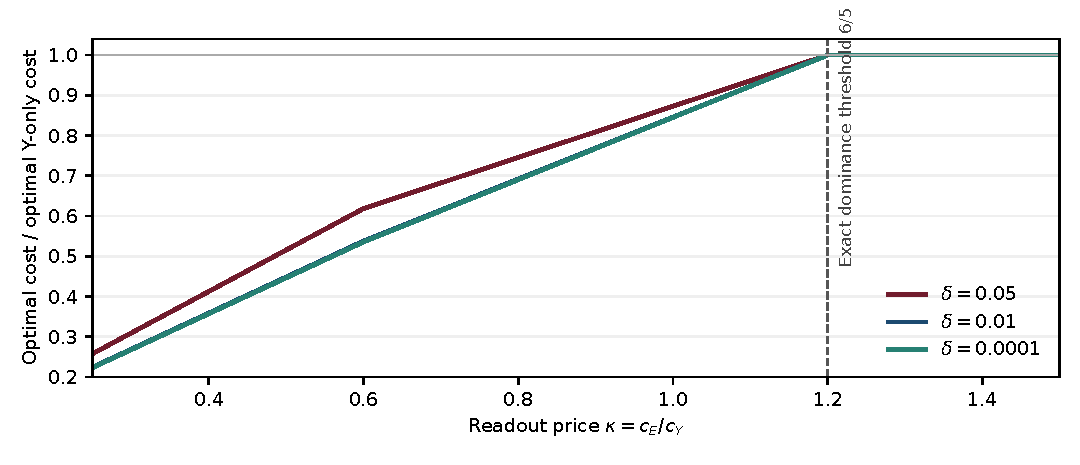
\includegraphics[width=.92\linewidth]{sharp_price_frontier.pdf}
 \caption{The exact confidence--price frontier of
 Theorem~\ref{thm:exact-price-frontier}, divided by the optimal $Y$-only
 cost. Every plotted price is checked by an exact rational primal--dual
 certificate. Lines join those samples; the equality plateau for
 $\kappa\geq6/5$ is proved for all prices, not inferred from the plot.
 The comparison concerns the two declared quantum readouts.}
 \label{fig:sharp-price-frontier}
\end{figure}

\paragraph{What is established and what is new in this development.}
The LP/Bellman method and controlled measurement selection have prior
theory \citep{fauss2015,lisensor2019}; the comparison-of-experiments principle
is classical \citep{blackwell1953}. The developments established here are
the explicit horizon-to-minimax bounds for the stated catalogue, the
parity-based exact confidence--price frontier, and its exactly realized
$6/5$ transition with rational optimality certificates. These supply a sharp, reproducible
characterization inside a declared model. They do not establish a new
general computational-complexity separation or priority over all work on
sequential experimental design.


\subsection{What the extension establishes}
The phase theorem remains a closed-form result for a restricted model.
The occupation and Bellman statements apply to finite-dimensional,
priced observation catalogues; the memory theorem permits collective
measurements inside blocks of growing size. These results make explicit
which arguments use qubit geometry, reflection symmetry, calibration,
or memory restrictions. They do not establish unrestricted quantum
computational speedups or solve arbitrary composite state families.
Composite sequential quantum testing already has separate asymptotic
theory \citep{simpson2026}; the band-calibration corollary above gives
a specific robust finite-cost guarantee rather than claiming that theory
as new. The exact lattice frontier optimizes every finite confidence and positive
readout price within its two-action family. Its quantum realizability
condition, the convergent catalogue programs, and the phase resource law
provide distinct levels of characterization; none silently enlarges the
admissible experiment class of another.


\section{From a utility margin to the phase experiment}\label{sec:amplitude-case}
Suppose two actions have utilities $u_1=a_h$ and $u_0=a_0$, where the
known candidate probabilities are $a_\pm=a_0\pm\Delta$ with
$0<a_-<a_+<1$. The unknown sign is the better-action label and the
utility margin is exactly $\Delta$.

\begin{proposition}[Calibrated margin-to-phase reduction]\label{prop:encoding}
Assume access to the rotations $U_{\mathrm{prep},h}=e^{-i\theta_hY}$,
their inverses and controlled uses, where $\theta_h=\arcsin\sqrt{a_h}$.
Then the circuit below realizes the phase-block model with
\begin{equation}\label{eq:margin-conversion}
 \mu=\frac{\arcsin\sqrt{a_0+\Delta}-\arcsin\sqrt{a_0-\Delta}}2
 =\frac{\Delta}{2\sqrt{\xi(1-\xi)}}
\end{equation}
for some $\xi\in(a_-,a_+)$. If $[a_-,a_+]\subset[\eta,1-\eta]$,
$0<\eta\leq1/2$, then
\[
 \Delta\leq\mu\leq\frac{\Delta}{2\sqrt{\eta(1-\eta)}}.
\]
Whenever $\mu\leq1/8$, the main frontier results apply with this
conversion and the priced circuit primitives.
\end{proposition}
\begin{proof}
The derivative of $f(a)=\arcsin\sqrt a$ is
$1/[2\sqrt{a(1-a)}]$. The mean-value theorem proves the identity and
the bounds. The controlled-kickback calculation below proves the exact
statistical reduction, including its noise model.
\end{proof}

This reduction assumes calibrated candidate values. The bias lemma in
Appendix~\ref{sec:identification} supplies an identification obstruction
when all access is corrupted by an unknown discrepancy; it does not
turn a composite unknown-gap problem into the calibrated two-point model.
The observable-transfer and perturbation lemmas in the appendices can
certify a decision margin, but coherent access must still be supplied.

\subsection{A worked amplitude-oracle construction}
The following example connects the rotation in amplitude estimation to
the restarted decision model with an explicit circuit and a direct
Bernoulli sampling comparator. Its access assumptions are part of the
example. Let $a_h\in\{a_-,a_+\}$, with
\[
 a_-=0.036,\qquad a_+=0.044,\qquad a_0=0.04,
 \qquad \theta_h=\arcsin\sqrt{a_h}.
\]
The task is to identify the unknown sign $h$ with error at most $\delta$
under either hypothesis. The two candidate amplitudes are known; the
unknown sign is accessible only through the specified oracle interface.
A classical call returns an independent $\operatorname{Bern}(a_h)$ sample
at unit cost. The coherent interface provides the one-qubit preparation
$U_{\mathrm{prep},h}=e^{-i\theta_hY}$, its inverse, and the required
controlled operations. Thus
\[
 U_{\mathrm{prep},h}\ket{0}
 =\cos\theta_h\ket{0}+\sin\theta_h\ket{1},
 \qquad
 Q_h=U_{\mathrm{prep},h}ZU_{\mathrm{prep},h}^{\dagger}Z
 =e^{-2i\theta_hY}.
\]
This $Q_h$ is the amplitude-amplification iterate, with eigenvalues
$e^{\pm2i\theta_h}$. The fixed state
$\ket{y_-}=(\ket{0}-i\ket{1})/\sqrt2$ is an eigenvector with eigenvalue
$e^{2i\theta_h}$ under both hypotheses. Both rotations have the same
known generator $Y$, so this eigenvector is independent of the unknown
$h$. Preparing it is an explicit feature of the one-qubit interface.
For a general multi-qubit expectation encoding, the normalized good and
bad components may be unknown or depend on $h$. Its corresponding
amplitude-amplification eigenstates need not be available for free:
preparing them is an additional task whose access requirements and cost
must be included. The construction here assumes the specified rotation
interface rather than such an eigenstate-preparation oracle.

Set
\begin{equation}\label{eq:case-angle}
 \overline\theta=\frac{\theta_++\theta_-}{2},\qquad
 \mu=\frac{\theta_+-\theta_-}{2}
 \approx0.01021868765.
\end{equation}
Prepare an ancilla in $\ket{+}$ and the target in $\ket{y_-}$.
Apply $t$ controlled uses of $Q_h$ and the known ancilla phase correction
$\operatorname{diag}(1,e^{-2it\overline\theta})$. Up to the unchanged
target state, the ancilla becomes
\begin{equation}\label{eq:case-kickback}
 \frac{\ket{0}+e^{2it(\theta_h-\overline\theta)}\ket{1}}{\sqrt2}
 =\frac{\ket{0}+e^{2ih\mu t}\ket{1}}{\sqrt2}.
\end{equation}
If independent pure dephasing multiplies the ancilla off-diagonal entry
by $e^{-\gamma}$ per controlled iterate, measuring $Y$ gives a sign
$W_t\in\{-1,+1\}$ satisfying
\[
 \E_h W_t=h e^{-\gamma t}\sin(2\mu t),\qquad
 X_t=(1+W_t)/2.
\]
This is exactly~\eqref{eq:bernoullimodel}. The controlled phase kickback
in~\eqref{eq:case-kickback} is essential to this normalization: simply
replacing an uncontrolled Grover iterate by the phase gate of
Section~\ref{sec:blockmodel} would introduce a factor of two in its
rotation parameter. For a general expectation encoding, efficient
preparation of an appropriate eigenstate and the cost of controlled
access require separate justification.

For a dimensionless cost example, take $D=256$, $c_0=20$, $c_1=10$,
and $\delta=0.01$. The restart cost includes the ancilla and target
preparation and readout. The per-iterate cost includes controlled
$U_{\mathrm{prep},h}$, its inverse, the reflections, and the phase
correction. These are assumed aggregate costs, not measured gate times.
The phase restriction gives $\overline D=38$. The coherent bounds in
Table~\ref{tab:amplitude-case} are obtained by enumerating every allowed
integer depth in~\eqref{eq:mainfrontier}.

\paragraph{A direct Bernoulli comparator.}
The direct samples have means $a_\pm$, rather than the symmetric
phase-matched means in Section~\ref{sec:comparison-sampling}. Write
\begin{equation}\label{eq:case-bernoulli-kl}
 \begin{split}
 J_+&=D_{\mathrm{KL}}(\operatorname{Bern}(a_+)\|
                      \operatorname{Bern}(a_-)),\\
 J_-&=D_{\mathrm{KL}}(\operatorname{Bern}(a_-)\|
                      \operatorname{Bern}(a_+)).
 \end{split}
\end{equation}
Let $C_{R,\delta}^\star$ be the minimax expected number of such samples,
over all sequential tests with both errors at most $\delta$. Applying
the stopped-transcript argument separately under both hypotheses gives
\begin{equation}\label{eq:case-classical-lower}
 C_{R,\delta}^\star\geq
 L_R:=\max\left\{\frac{k_\delta}{J_+},\frac{k_\delta}{J_-}\right\}.
\end{equation}
Both directions matter: the two divergences are unequal.

An explicit upper bound also makes a disadvantage certificate possible.
Set $B_\delta=\log(1/\delta)$ and stop the Bernoulli log-likelihood ratio
at its first exit from $(-B_\delta,B_\delta)$, choosing the boundary's
sign. The likelihood-ratio martingale bounds each error by
$e^{-B_\delta}=\delta$. A positive increment has size
$u_+=\log(a_+/a_-)$ and a negative increment has magnitude
$u_-=\log((1-a_-)/(1-a_+))$. Bounded overshoot and Wald's identity give
\begin{equation}\label{eq:case-classical-upper}
 C_{R,\delta}^\star\leq
 U_R:=\max\left\{\frac{B_\delta+u_+}{J_+},
                  \frac{B_\delta+u_-}{J_-}\right\}.
\end{equation}
Indeed, the mean log-likelihood increments are $J_+$ under $h=+1$
and $-J_-$ under $h=-1$, whereas the corresponding terminal signed
log likelihood is at most $B_\delta+u_+$ or $B_\delta+u_-$.
The exit time has finite mean for these distinct interior Bernoulli
parameters. The bounds do not require equal achieved errors or zero
overshoot.

Numerically, $J_+\approx0.000862798$ and
$J_-\approx0.000809235$, giving
\begin{equation}\label{eq:case-classical-values}
 5564.8\approx L_R\leq C_{R,0.01}^\star\leq U_R\approx5701.1.
\end{equation}
\begin{table}[htbp]
\centering\small
\setlength{\tabcolsep}{4pt}
\begin{tabular}{rrrrrrl}
\toprule
$\gamma$ & $t_M$ & $t_U$ & $L_Q$ & $L_M$ & $U_Y$ & Certificate\\
\midrule
0.004 & 38 & 31 & 1,655.29 & 2,016.58 & 2,475.90 & Y cost gain\\
0.015 & 29 & 30 & 4,382.91 & 5,059.73 & 5,130.65 & Y cost gain\\
0.020 & 24 & 22 & 5,765.69 & 6,658.96 & 6,722.91 & \shortstack{Every readout\\loses}\\
\bottomrule\end{tabular}
\caption{Calibrated amplitude-oracle example at $\delta=.01$, $D=256$,
$c_0=20$, $c_1=10$, and unit direct-sampling price.
$t_M$ maximizes measured information; $t_U$ minimizes the fixed-$Y$ counting cost.
$L_Q=k_\delta/I_Q$ and $L_M=k_\delta/I_M$ lower-bound every allowed single-block readout.
The $L_M$ entries use interval upper bounds on $I_M$ and are rounded down;
other entries are rounded approximations. Direct-sampling bounds are
$L_R\approx5564.8$ and $U_R\approx5701.1$. Gain means $U_Y<L_R$;
the final loss is certified with outward rounding in~\eqref{eq:strong-loss}.}
\label{tab:amplitude-case}
\end{table}

\begin{samepage}
At $\gamma=0.004$, the certified sampling-to-coherent minimax cost
ratio is at least $L_R/U_Y\approx2.2476$. At $\gamma=0.015$,
$U_Y\approx5130.6<L_R$, so the advantage certificate still holds.
At $\gamma=0.020$, interval evaluation of
\eqref{eq:rate-enclosure} and~\eqref{eq:case-classical-upper} gives the
conservatively rounded certificate
\begin{equation}\label{eq:strong-loss}
 \boxed{C_{M,.01}^\star\geq6658.96>5701.07\geq C_{R,.01}^\star.}
\end{equation}
The explicit classical test is therefore cheaper than every restarted-block
protocol with adaptive single-block readout at the common stated price.
The lower-bound margin relative to $U_R$ is about $16.80\%$.
The simpler quantum bound $L_Q\approx5765.7$ already certifies a loss,
but with only a $1.13\%$ margin. At this confidence the explicit
$Y$ cost $U_Y\approx6722.9$ is within about one percent of the stronger
general-readout lower bound. This comparison excludes cross-block
quantum memory and error correction.\par
\end{samepage}

This construction prices a calibrated amplitude oracle against access
to independent samples of its encoded Bernoulli variable. It does not
establish an application speedup from a classical description of a
general distribution: constructing the oracle, justifying its noise
model, and comparing with algorithms using additional input structure
remain separate tasks. The companion \texttt{verify\_case\_study.py}
checks the two-qubit circuit with its dephasing channel, independently
solves the stopping-chain equations, and supplies the fixed-$Y$ and
sampling quantities. The final measurement columns are generated by
\texttt{verify\_interval\_certificates.py}.

\section{Reproducible cost comparisons}\label{sec:researchresults}
The accompanying \texttt{research\_checks.py} evaluates the exact
Bernoulli model, optimizes over every allowed integer depth, and computes
both sides of \eqref{eq:mainfrontier}. The displayed confidence level is
$\delta=0.01$, the hardware depths are listed in the parameter table, and the sampling
cost is $c_C=1$. All quantities are dimensionless model costs.
The examples are analytical model calculations, not quantum-hardware
measurements or application benchmarks.

\begin{table}[htbp]
\centering\small
\begin{tabular}{lrrrrr}
\toprule
Setting & $\mu$ & $\gamma$ & $D$ & $c_0$ & $c_1$\\
\midrule
Ideal & 0.02 & 0 & 256 & 0 & 1\\
Shallow & 0.002 & 0 & 16 & 0 & 1\\
Noisy & 0.005 & 0.02 & 256 & 0 & 1\\
Costly & 0.02 & 0.04 & 256 & 50 & 5\\
Restarts & 0.01 & 0.01 & 256 & 100 & 1\\
\bottomrule\end{tabular}
\caption{Parameters of the reproducible decision experiments.}
\end{table}
\begin{table}[htbp]
\centering\small
\setlength{\tabcolsep}{3pt}
\begin{tabular}{lrrrrrrl}
\toprule
Setting & $t_\star$ & $t_U$ & POVM cost & $L_Y$ & $U_Y$ & $I_Y/I_C$ & Certificate\\
\midrule
Ideal & 19 & 18 & $\leq 69.1$ & 73.4 & 80.5 & 19.170 & Depth gain\\
Shallow & 16 & 16 & $\leq 7{,}815.2$ & 8,795.3 & 8,828.9 & 16.000 & Depth gain\\
Noisy & 24 & 26 & $\geq 2{,}476.1$ & 2,479.7 & 2,502.0 & 9.080 & Depth gain\\
Costly & 15 & 17 & $\geq 2{,}825.4$ & 2,834.6 & 2,908.6 & 0.496 & Every readout loses\\
Restarts & 39 & 39 & $\geq 1{,}254.0$ & 1,268.9 & 1,443.3 & 4.436 & Depth gain\\
\bottomrule\end{tabular}
\caption{Bounds on optimal expected cost at $\delta=0.01$.
$t_\star,t_U,L_Y,U_Y$ concern fixed $Y$. The POVM-cost column bounds
$C^\star_{M,\delta}$ at the same block price. For $\gamma=0$ it is the
zero-error upper bound of Proposition~\ref{prop:usd}, minimized over depth
and rounded up. For $\gamma>0$ it is $k_\delta/I_M$ from
Theorem~\ref{thm:measured}, evaluated using outward interval upper bounds
on $I_M$ at every allowed depth and rounded down.
Other numerical columns are rounded approximations.
The sampler costs are $U_C\approx1422.7$ (Ideal, Costly),
$140{,}889.3$ (Shallow), $22{,}542.6$ (Noisy), and $5636.0$ (Restarts).
Depth gain means $U_Y<L_C$; in the Costly row,
$k_\delta/I_M>U_C$ certifies a loss for every single-block readout.}
\label{tab:researchresults}
\end{table}


In the two noiseless rows the zero-error readout is already cheaper than
the fixed-$Y$ lower bound at $\delta=0.01$. For the Noisy, Costly, and
Restarts rows, the stronger measured-information lower bounds are
approximately $2476.2$, $2825.4$, and $1254.0$. The table uses downward
rounding of outward interval bounds, rather than these nearest-rounded
approximations. The excess optimal information rate
$100(I_M/I_Y-1)$ is approximately $0.14\%$, $0.33\%$, and $1.18\%$,
respectively. Thus optimizing the readout gives only a small
high-confidence rate improvement in these three examples; this is not
a bound on the finite-confidence cost improvement. In the Costly row,
the measured-information lower bound exceeds the sampler's achievable
cost, certifying a loss for every single-block readout at the stated
common price.


\begin{figure}[htbp]
 \centering
 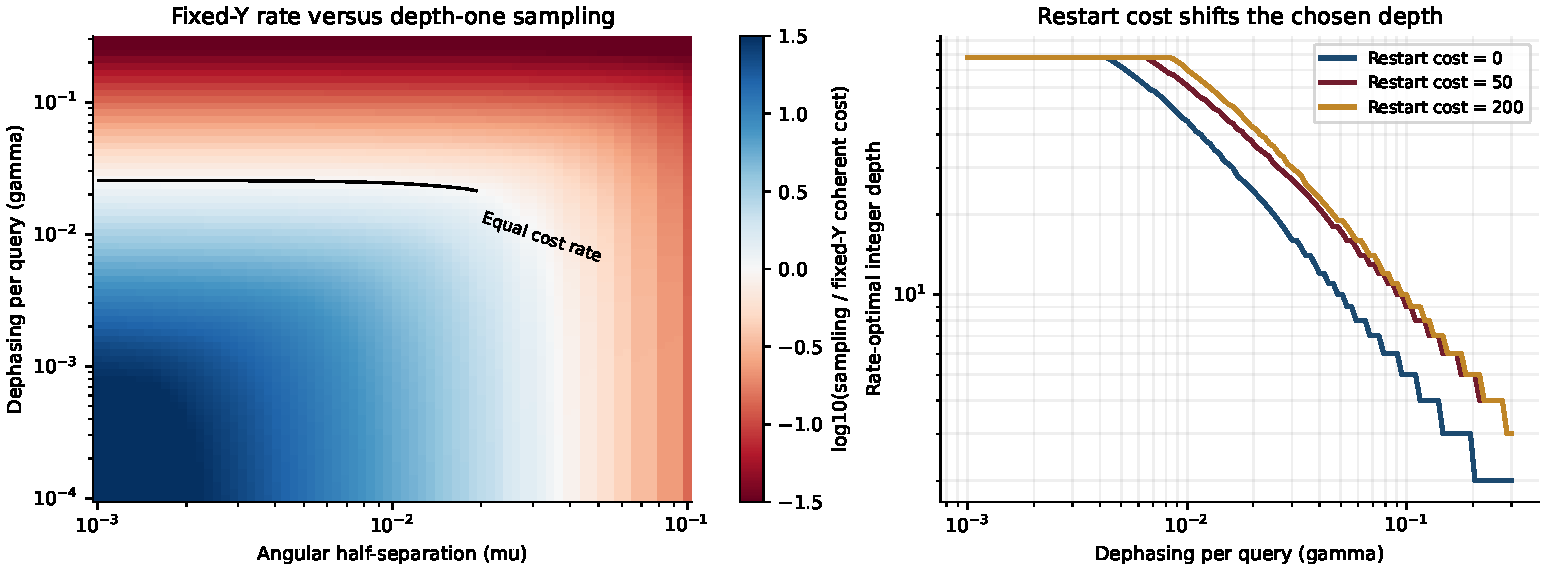
\includegraphics[width=\linewidth]{quantum_decision_frontier.pdf}
 \caption{Exact information-rate comparisons in the specified experiment.
 Left: the asymptotic sampling-to-coherent cost ratio $I_Y/I_C$
 as angular margin and dephasing change, at $D=256$, $c_0=50$, $c_1=5$.
 The unit contour separates favorable and unfavorable rates.
 Right: the optimizing integer depth versus noise at $\mu=0.005$,
 $D=256$, $c_1=1$, for several restart costs. These plots show model
 boundaries, not measured hardware performance.}
 \label{fig:researchfrontier}
\end{figure}

The verification script independently solves the absorbing random-walk
equations for the stopping rule, checks the exact error and expected cost,
tests the perturbation inequality on complex matrices and vectors, checks
the sensitivity derivative by finite differences, and verifies the
confidence allocation against numerical optimization. It also tests the
envelope minimizer. These checks supplement, rather than replace, the proofs.
The additional \texttt{verify\_boost.py} checks the sharp envelope, the
finite-confidence sampling certificate, and the robustness cost ratio.
It includes the exact counterexample in~\eqref{eq:boost-counterexample}
and independent absorbing-chain calculations of stopping probabilities
and durations. The deterministic outputs are supplied in
\texttt{boost\_verification\_results.json}.
The additional \texttt{verify\_case\_study.py} verifies the controlled
amplitude-oracle circuit, its direct sampling comparator, and the
constructive integer-depth choice in Corollary~\ref{cor:effective}.
Its outputs are \texttt{case\_study\_results.json} and
\texttt{case\_study\_results\_table.tex}; the case study appears in
Section~\ref{sec:amplitude-case}.


\subsection{Readout calculations and finite-noise crossover}
The additional \texttt{verify\_measurements.py} constructs density matrices
and POVM effects directly. It checks quantum relative entropy by matrix
diagonalization, the recorded-axis measurement probabilities, positivity
and completeness of the unambiguous POVM, and the exact conclusive error
and cost under dephasing. It also checks the drift and Hellinger identities
used in the adaptive proof and reports numerical projective-readout
rates as achievable candidates. The final operational-rate calculation
uses the global bound in Proposition~\ref{prop:residual}, rather than
treating an optimizer's convergence flag as a certificate.
The additional \texttt{verify\_table\_rates.py} evaluates every allowed
depth for the three noisy rows in Table~\ref{tab:researchresults},
encloses their measured rates with outward interval arithmetic, and
regenerates the stronger cost lower bounds. It also checks the
rate-improvement percentages and the reported numerical band for the
uniform scale.
The additional \texttt{verify\_readout\_patch.py} independently solves the
SLD matrix equation, tests the chi-square inequality on random POVMs,
checks the factor-three condition and the noiseless resource bound,
and recomputes the measurement-independent cost certificates.
\begin{table}[htbp]
\centering\small
\begin{tabular}{rrrrl}
\toprule
$\gamma$ & First-conclusive error & Expected cost & Pure-state cost & Meets $\delta=.01$\\
\midrule
0 & 0.000000 & 69.050 & 69.050 & Yes\\
1e-06 & 0.000020 & 69.048 & 69.050 & Yes\\
0.0001 & 0.001996 & 68.905 & 69.050 & Yes\\
0.001 & 0.019423 & 67.641 & 69.050 & No\\
0.01 & 0.152991 & 57.949 & 69.050 & No\\
\bottomrule\end{tabular}
\caption{Exact first-conclusive readout at $\mu=.02$, $t=19$, $c_0=0$, $c_1=1$.
The decreasing mean cost at higher noise reflects more conclusive outcomes, including errors;
rows failing the target are not admissible upper bounds at that confidence.}
\label{tab:crossover}
\end{table}

\begin{figure}[htbp]
\centering
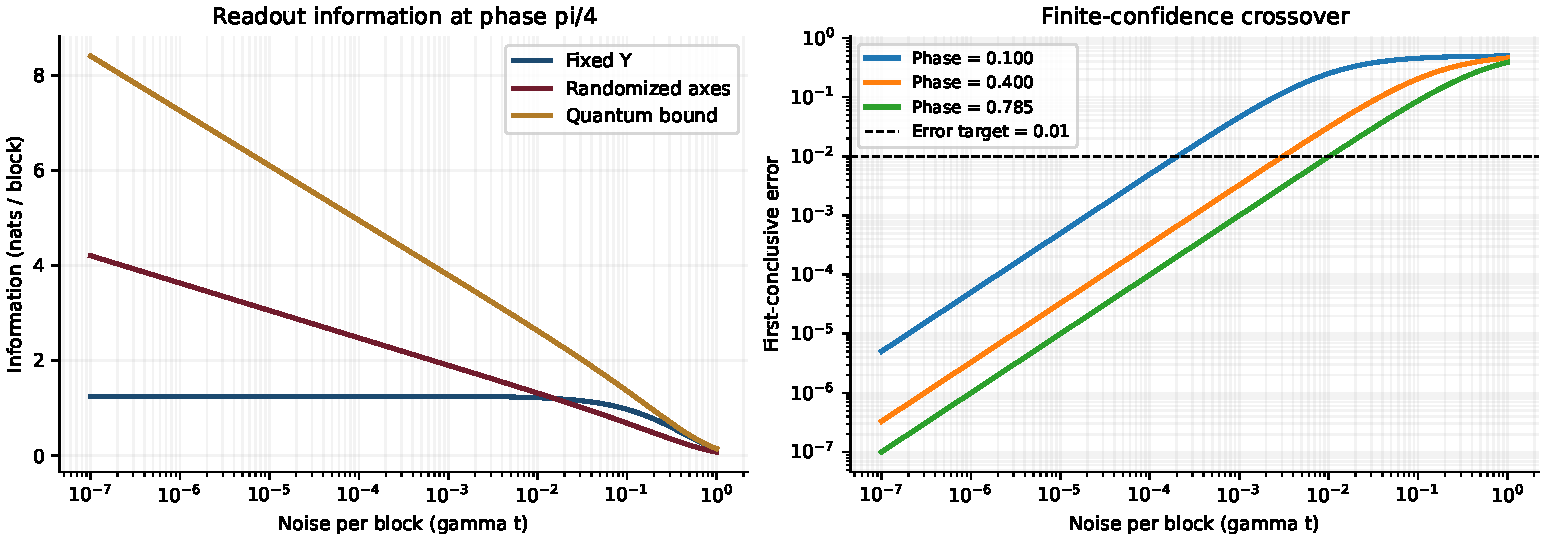
\includegraphics[width=\linewidth]{measurement_frontier.pdf}
\caption{Readout dependence in the mathematical block model.
Left: $Y$, randomized-axis, and quantum relative information at
$\vartheta=\pi/4$ as $\gamma t$ varies. The quantum curve is an upper
bound on single-block measured information.
Right: the exact first-conclusive error for several phase angles.
The horizontal line is the target $\delta=0.01$.}
\label{fig:measurement}
\end{figure}
\subsection{Certified operational rates}
The script \texttt{verify\_operational\_frontier.py} searches the planar
measurement angle and refines its variational stationary point in
80-decimal arithmetic. It evaluates 348 allowed depths across the six
settings in Table~\ref{tab:operational-rates} and checks the
stopped-affinity telescope on 80 finite adaptive measurement trees.
\begin{table}[htbp]
\centering\small
\setlength{\tabcolsep}{4pt}
\begin{tabular}{lrrrrr}
\toprule
Setting & $t_M$ & $I_Y$ & $I_M$ & $I_Q$ & $I_M/I_Y$\\
\midrule
Low noise & 19 & 0.061046723 & 0.13874043 & 0.17350442 & 2.272692\\
Moderate noise & 19 & 0.038805831 & 0.040601966 & 0.048686371 & 1.046285\\
Noise limited & 25 & 0.00029368313 & 0.00029375217 & 0.00034732005 & 1.000235\\
Amplitude, $\gamma=0.004$ & 38 & 0.0020961369 & 0.0022330946 & 0.0027204927 & 1.065338\\
Amplitude, $\gamma=0.015$ & 29 & 0.00088329905 & 0.00089001134 & 0.0010274495 & 1.007599\\
Amplitude, $\gamma=0.020$ & 24 & 0.00067308865 & 0.0006762638 & 0.00078103674 & 1.004717\\
\bottomrule\end{tabular}
\caption{Operational rates at their separately optimized depths; values are rounded.
The first three rows use $(\mu,\gamma)=(.02,.0001),(.02,.01),(.002,.02)$,
$D=256$, $c_0=0$, $c_1=1$. Amplitude rows use the parameters of
Table~\ref{tab:amplitude-case}. Residual bounds are evaluated at high precision;
outward interval arithmetic certifies the three amplitude rows.
$I_M$ describes high-confidence information per cost, not an exact finite-confidence cost.}
\label{tab:operational-rates}
\end{table}


For the three amplitude cases,
\texttt{verify\_interval\_certificates.py} evaluates the probabilities,
relative entropies, generalized-eigenvalue spread, and gradient residual
using 65-decimal outward interval arithmetic. Every allowed depth is
included, with exact decimal inputs $a_-=.036$, $a_+=.044$ and the
interval-converted phase separation. The code encloses $I_M$ using
\eqref{eq:rate-enclosure} and obtains a lower cost bound by dividing
$k_\delta$ by the upper endpoint. The supplied result file records the
angle and rate enclosure at every depth. Table~\ref{tab:amplitude-case}
reports the resulting lower costs, and~\eqref{eq:strong-loss} uses
outward rounding. This is an interval evaluation of proved inequalities,
not a proof-assistant formalization.

The rate-maximizing depths need not agree: at $\gamma=.020$ in the
amplitude example, $t_M=t_\star=24$, whereas the quantum bound is
maximized at depth $20$ and the finite-confidence counting cost at depth
$t_U=22$. Nor does equality of depths imply equality of measurement
information: Corollary~\ref{cor:strict-rates} remains strict.

\subsection{Matrix identities and drifting signals}
The script \texttt{verify\_refinements.py} checks the partial-transpose
counterexample, dephasing composition, and the explicit generalized
eigenvalue formula. It also evaluates worst-case finite-horizon dynamic
programs over the admissible signal interval. These optimize both error
and expected duration over adaptive choices, and agree with the bounds
in Proposition~\ref{prop:drifting-visibility}. The script reports the
residual from a coarse angular grid separately from the refined
stationary-point calculation; a grid maximum alone need not meet a
prescribed residual tolerance.

\subsection{Checks of the uniform resource law}
The script \texttt{verify\_joint\_frontier.py} independently checks the
scalar divergence inequality, mixed-state fidelity and arbitrary POVM
ratios, pointwise information bounds, and finite adaptive history trees.
It solves finite absorbing Markov systems to check the exact error and
mean cost of conclusive counting, and sweeps the signal, noise, depth,
restart price, and confidence over multiple scales. These numerical
checks supplement the analytical proofs and do not infer uniform
constants from a finite grid. Figure~\ref{fig:joint-frontier} compares
analytical lower bounds and attainable upper costs in a depth-limited
example; the machine-readable results include the full input grid.
\begin{figure}[htbp]
\centering
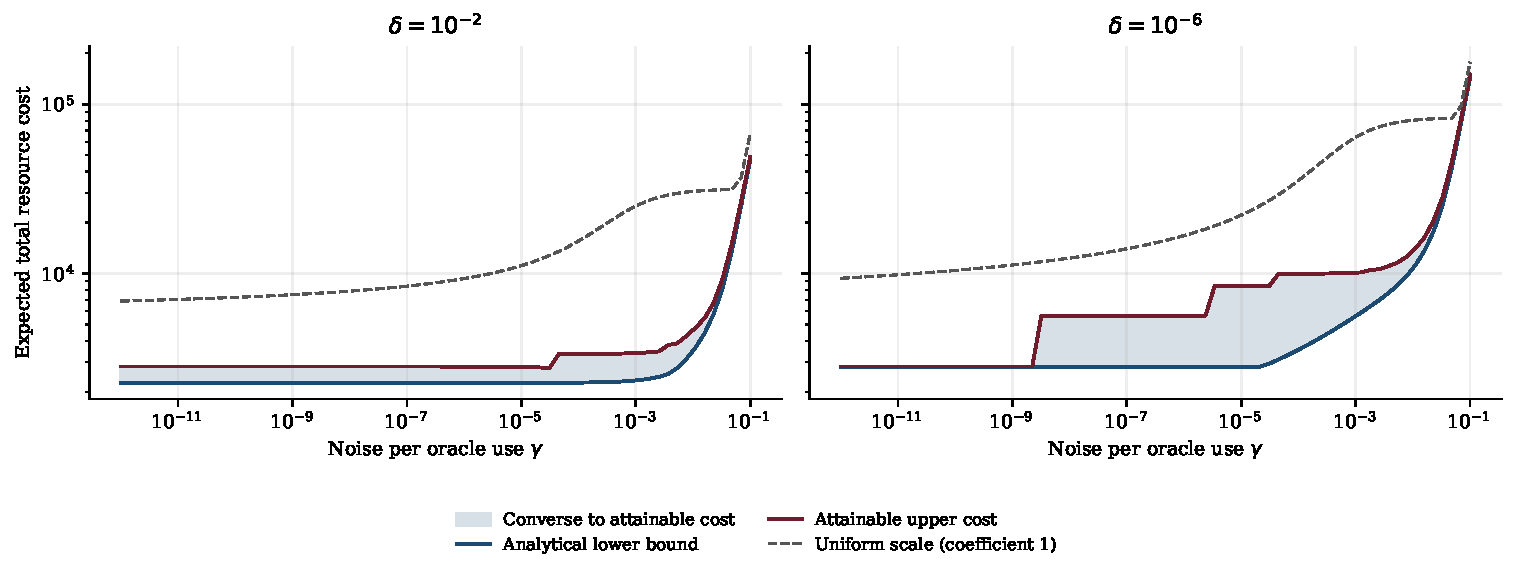
\includegraphics[width=\linewidth]{joint_frontier.pdf}
\caption{Uniform transition in a depth-limited example:
$\mu=.005$, $D=16$, $c_0=20$, $c_1=1$.
The shaded band runs from the maximum of the affinity and KL lower
bounds to the smaller achievable cost of $Y$ and conclusive counting,
optimized over the allowed depths. The KL bound uses the explicit
pointwise upper bound in~\eqref{eq:pointwise-complete}.
The dashed curve is the scale $A_{\rm eff}[1+\log(1/\delta)/G_{\rm eff}]$
with coefficient one; it is not itself a bound. Values are high-precision
numerical evaluations of proved inequalities, not outward interval
certificates or measurements of hardware performance.}
\label{fig:joint-frontier}
\end{figure}
\subsection{Checks of the extended theory}
The script \texttt{verify\_deep\_extensions.py} encloses the sharper
constants with outward intervals and checks independent optimized
measurement values against the new pointwise bounds. Its parameter
grid includes phase-cap discontinuities and tiny positive noise. It
certifies the readout-overhead examples at every allowed depth and
checks feasible LP duals and randomized designs for the noncommuting
three-state experiment. Independent adaptive trees verify occupation
and affinity identities. Exact finite-policy envelopes are compared
with interpolated Bellman recursion at small horizons. These numerical
checks support the proofs; only the explicitly marked interval
calculations are claimed as numerical certificates.

The separate script \texttt{verify\_sharp\_characterization.py} verifies
exact rational barrier policies and their global supporting lines,
including the infinite-barrier cutoff. It checks the quantum realization,
72 additional parameter combinations, and 303 price-curve points.
Independent absorbing-chain systems reproduce the error and cost formulas;
a full interval Bellman recursion at horizon 96 agrees with all nine
reported optima within $10^{-12}$. Enumeration of 2942 two-stage trees
checks the conditional minimax formulation independently. Small three-label
LPs check the general likelihood-vector dual. The latter LP solver checks
are floating-point diagnostics; the displayed optimal-cost certificates
use exact rational arithmetic.
\FloatBarrier

\section{Conclusions and scope}
Two different levels of characterization are now available. For the
likelihood-lattice family, Theorem~\ref{thm:exact-price-frontier} gives
an exact finite-confidence minimax answer for every positive readout
price. The stopped drift fixes the information budget, and parity fixes
the minimum number of single-step measurements. Their combination yields
a converse attained by mixing at most two barrier policies. The result
includes randomized stopping and all adaptive choices between the two
readouts; it is not restricted to a nominated threshold rule.

The family has an explicit quantum realization region
(Proposition~\ref{prop:lattice-realizability}). A full-rank noncommuting
example exhibits a sharp price threshold of $6/5$: at or above that
price the additional readout cannot help at any confidence, while below
it the high-confidence cost ratio is $5\kappa/6$. At equal prices the
limiting reduction is $1/6$. Exact rational primal--dual certificates
and a separate interval Bellman calculation verify the finite-confidence
examples. The optimality statement concerns the declared readout catalogue,
not every POVM on those states.

For the calibrated phase oracle, Theorem~\ref{thm:uniform-cost} supplies
matching orders across noise, depth, signal and confidence, with cost
scale $A_{\rm eff}[1+\log(1/\delta)/G_{\rm eff}]$. An affinity converse
controls the base scale, a KL converse controls confidence, and a
fixed-depth counting protocol attains their combined order. Global
multipliers $1/70$ and $42$, and a factor-27 fixed-depth bracket, remain
conservative universal comparisons. They do not become exact constants
because the separate lattice model is solvable. At zero noise the
exact zero-error cost is finite; at fixed positive noise it is infinite.
Measured relative entropy determines the high-confidence coefficient.

Beyond those qubit models, the occupation LP is a tractable converse
for priced finite-dimensional catalogues. The full policy programs in
Theorem~\ref{thm:catalogue-exact} converge to the actual multi-hypothesis
minimax value, with explicit error; uniform pairwise separation yields
exponential convergence. This gives a general characterization, not a
claim of efficient enumeration for every catalogue. A certified signal
floor protects counting against predictable calibration drift. Collective
blocks recover the quantum information rate only with the stated order
of confidence and memory limits and with their entry cost included.

Application-level advantage still requires priced coherent access and
a classical comparator with comparable input information. The robust
band result is not a general composite minimax law, and collective blocks
do not describe arbitrary persistent quantum memory or error correction.
The paper's exact frontier, uniform resource law and numerical certificates
are mathematical cost statements under declared interfaces. Their
foundations in sequential testing, optimization and experiment comparison
are credited; these results do not constitute a general quantum-complexity
separation or a hardware benchmark.

\FloatBarrier
\appendix
\section{The observable geometry of a decision}\label{sec:decisiongeometry}
Let $\mathcal A$ be a finite action set. For a density matrix $\rho$, define
utilities
\begin{equation}
 u_a(\rho)=\Tr(\rho O_a),\qquad 0\preceq O_a\preceq I.
\end{equation}
Let $a^\star(\rho)$ be a utility-maximizing action, and define regret
\begin{equation}
 \mathcal R(\rho,a)=u_{a^\star(\rho)}(\rho)-u_a(\rho).
\end{equation}
When the optimum is unique, its margin is
\begin{equation}
 \Delta(\rho)=\min_{b\ne a^\star(\rho)}
 \Tr\!\left[\rho(O_{a^\star(\rho)}-O_b)\right]>0.
\end{equation}

\begin{definition}[Decision pseudometric]
For the specified action family, set
\begin{equation}\label{eq:decisionmetric}
 d_{\mathcal A}(\rho,\sigma)=
 \max_{a,b\in\mathcal A}
 \left|\Tr[(\rho-\sigma)(O_a-O_b)]\right|.
\end{equation}
Two states are decision-equivalent when this quantity vanishes.
\end{definition}
This is a pseudometric because it can be zero for distinct states.
It records only differences of utilities, since adding the same value to
every action changes no preference. It depends on the real linear space
\begin{equation}
 \mathcal V_{\mathcal A}=
 \operatorname{span}_{\R}\{O_a-O_b:a,b\in\mathcal A\}.
\end{equation}
This is an operator subspace, not necessarily an algebra: multiplication
closure is not assumed.

\begin{theorem}[Transfer of decisions]\label{thm:decisiontransfer}
If $\widehat a$ is optimal for $\sigma$, then
\begin{equation}
 \mathcal R(\rho,\widehat a)\leq d_{\mathcal A}(\rho,\sigma).
\end{equation}
If $\rho$ has a unique optimal action and
$d_{\mathcal A}(\rho,\sigma)<\Delta(\rho)$, every optimal action for
$\sigma$ equals $a^\star(\rho)$. Moreover,
\begin{equation}
 d_{\mathcal A}(\rho,\sigma)\leq2D_{\mathrm{tr}}(\rho,\sigma),
 \qquad D_{\mathrm{tr}}(\rho,\sigma)=\tfrac12\|\rho-\sigma\|_1.
\end{equation}
\end{theorem}
\begin{proof}
With $G=O_{a^\star(\rho)}-O_{\widehat a}$, optimality under $\sigma$
gives $\Tr(\sigma G)\leq0$. Therefore
\[
 \mathcal R(\rho,\widehat a)
 =\Tr[(\rho-\sigma)G]+\Tr(\sigma G)
 \leq|\Tr[(\rho-\sigma)G]|.
\]
If $\widehat a$ were suboptimal under $\rho$, its regret would be at least
$\Delta(\rho)$, contradicting the strict bound. Finally,
$-I\preceq G\preceq I$ implies $\|G\|\leq1$, and trace-norm duality gives
$|\Tr[(\rho-\sigma)G]|\leq\|\rho-\sigma\|_1$.
\end{proof}

\begin{remark}[Spectral-spread refinement]\label{rem:spread}
For a Hermitian operator $G$, define
$\operatorname{spr}(G)=\lambda_{\max}(G)-\lambda_{\min}(G)$.
The decision pseudometric in~\eqref{eq:decisionmetric} satisfies the sharper bound
\begin{equation}\label{eq:spread}
 d_{\mathcal A}(\rho,\sigma)\leq D_{\mathrm{tr}}(\rho,\sigma)
 \max_{a,b\in\mathcal A}\operatorname{spr}(O_a-O_b).
\end{equation}
Indeed, $\Tr(\rho-\sigma)=0$. For
$c=(\lambda_{\max}(G)+\lambda_{\min}(G))/2$, trace-norm duality gives
\[
 |\Tr[(\rho-\sigma)G]|
 =|\Tr[(\rho-\sigma)(G-cI)]|
 \leq\|\rho-\sigma\|_1\|G-cI\|
 =D_{\mathrm{tr}}(\rho,\sigma)\operatorname{spr}(G).
\]
The normalization $0\preceq O_a\preceq I$ used here implies
$-I\preceq O_a-O_b\preceq I$, hence a spread at most two.
Equation~\eqref{eq:spread} improves the coefficient whenever the largest
utility-difference spread is below two. If only $\|O_a\|\leq1$ were assumed,
the general spread bound would instead be four.
\end{remark}

A useful converse to the last implication fails. Let
$\rho=\ket{0}\bra{0}\otimes\ket{z}\bra{z}$ and
$\sigma=\ket{0}\bra{0}\otimes\ket{w}\bra{w}$ with $z\perp w$.
Their trace distance is one. If every action depends only on the first
qubit, then $d_{\mathcal A}(\rho,\sigma)=0$. Full-state accuracy can be
unnecessary for a decision.

\subsection{Small output dimension does not imply easy computation}
The decision quotient can have dimension one and still encode a difficult
problem. This blocks an overly optimistic interpretation of compression.

\begin{proposition}[One observable can retain quantum decision hardness]
Given a uniform polynomial-size quantum circuit $C$, let
$p_C$ be the probability that its designated output qubit is one.
Under the promise $p_C\geq2/3$ or $p_C\leq1/3$, choose between utilities
$u_1=p_C$ and $u_0=1-p_C$. This decision is complete for promise-BQP under the usual
classical reductions, and is hard for BQP languages, even though the utility-difference space is
one-dimensional and the margin is at least $1/3$.
\end{proposition}
\begin{proof}
A quantum computer decides the promise by repeated circuit execution.
Conversely, the acceptance circuit of any language in BQP gives an instance
of this promise problem by the definition of BQP. Choosing the better action
therefore decides the original language. The only difference observable is
$2\Pi_1-I$, and $|u_1-u_0|=|2p_C-1|\geq1/3$.
\end{proof}

Thus a classical polynomial-time algorithm for every such circuit input
would imply $\BPP=\BQP$. This is a conditional obstruction, not a proof of
that separation. A compact output can preserve hardness, and a large state
can be easy for a particular task.

\section{Bias can make a decision unidentifiable}\label{sec:identification}
Statistical error and model discrepancy have different logical roles.
More observations reduce sampling error. They cannot distinguish two
worlds that generate identical observations.

\begin{lemma}[An identification threshold]\label{thm:bias}
Suppose the true signed utility gap is $g\in\{-\Delta,+\Delta\}$,
where $\Delta>0$, but every allowed experiment depends on the instance
only through $z=g+b$, with an unknown deterministic discrepancy
$|b|\leq\beta$.
If $\beta\geq\Delta$, no randomized or quantum protocol can identify the
sign of $g$ with worst-case error below $1/2$.
If $\beta<\Delta$, then $\operatorname{sign}z=\operatorname{sign}g$ and
$|z|\geq\Delta-\beta$.
\end{lemma}
\begin{proof}
When $\beta\geq\Delta$, the positive world $(g,b)=(\Delta,-\Delta)$
and the negative world $(-\Delta,\Delta)$ both have $z=0$.
Every allowed interaction, including an adaptive one, is identical in the
two worlds. If a final rule returns positive with probability $q$, its
errors are $1-q$ and $q$, so their maximum is at least $1/2$.
When $\beta<\Delta$, the intervals
$[\Delta-\beta,\Delta+\beta]$ and
$[-\Delta-\beta,-\Delta+\beta]$ lie strictly on opposite sides of zero.
\end{proof}

The lemma is an identification result, not a noise-correction theorem.
Its premise that all access factors through $z$ is essential. An additional
calibration experiment that identifies $b$ can change the conclusion.
The residual gap $\Delta-\beta$ is also not automatically a phase angle.
A physical encoding must supply the conversion from utility differences
to distinguishable experimental parameters.

\section{Decision-sensitive perturbations of quantum linear algebra}\label{sec:decisionperturb}
Consider a desired normalized solution
\begin{equation}
 y=A^{-1}b,\qquad r_y=\|y\|>0,\qquad x=y/r_y,
\end{equation}
and a Hermitian utility-difference observable $G$.
The relevant scalar is $u=x^\dagger Gx$.
Suppose the actual unnormalized vector is $y'=y+e_y$.
Set $\zeta=e_y/r_y$ and $\eta_{\mathrm{pert}}=\|\zeta\|<1$, so
$x'=(x+\zeta)/\|x+\zeta\|$.

\begin{lemma}[An observable-sensitive perturbation certificate]\label{thm:perturb}
Let $R_G=\|(G-uI)x\|$ and $B_G=\|G-uI\|$. Then
\begin{equation}\label{eq:taskperturb}
 |x'^\dagger Gx'-x^\dagger Gx|
 \leq \frac{2R_G\eta_{\mathrm{pert}}+B_G\eta_{\mathrm{pert}}^2}{(1-\eta_{\mathrm{pert}})^2}.
\end{equation}
If $Gx=ux$, the leading term is quadratic:
\begin{equation}
 |u'-u|\leq\frac{B_G\eta_{\mathrm{pert}}^2}{(1-\eta_{\mathrm{pert}})^2}.
\end{equation}
\end{lemma}
\begin{proof}
Subtract $u$ after putting both expectations over the same denominator:
\begin{equation}
 u'-u=
 \frac{2\operatorname{Re}[x^\dagger(G-uI)\zeta]
       +\zeta^\dagger(G-uI)\zeta}{\|x+\zeta\|^2}.
\end{equation}
Cauchy--Schwarz bounds the numerator by
$2R_G\eta_{\mathrm{pert}}+B_G\eta_{\mathrm{pert}}^2$, while the reverse triangle inequality gives
$\|x+\zeta\|\geq1-\eta_{\mathrm{pert}}$.
\end{proof}

For actions indexed by $a$, apply this bound to each
$G_{ab}=O_a-O_b$. If the bound is smaller than every gap separating the
optimal action from its competitors, the action is unchanged.
This certificate can be much less conservative than controlling every
coordinate of $x$ or applying one global operator-norm error bound.

\subsection{From matrix and right-hand-side error to the certificate}
Let the implemented system be $(A+E)y'=b+e$, and assume
$q=\|A^{-1}E\|<1$. The resolvent identity gives
\begin{equation}
 y'-y=(I+A^{-1}E)^{-1}A^{-1}(e-Ey),
\end{equation}
so
\begin{equation}\label{eq:etaresolvent}
 \eta_{\mathrm{pert}}\leq
 \frac{\|A^{-1}\|}{1-q}
 \left(\frac{\|e\|}{\|y\|}+\|E\|\right).
\end{equation}
Combining \eqref{eq:etaresolvent} with \eqref{eq:taskperturb} is valid
when the resulting upper bound on $\eta_{\mathrm{pert}}$ is below one.
A sharper directional estimate of $y'-y$ can replace the norm bound.

At first order,
\begin{equation}\label{eq:decisionderivative}
 du=\frac{2}{r_y}\operatorname{Re}
 \left[x^\dagger(G-uI)A^{-1}(db-dA\,y)\right].
\end{equation}
For perturbations of $b$ alone, the absolute local sensitivity is
\begin{equation}
 K_{G,b}=\frac{2}{r_y}
 \left\|A^{-\dagger}(G-uI)x\right\|.
\end{equation}
This depends on the observable and the solution direction, not only on
$\kappa(A)$. It is a conditioning statement, not a construction of a
linear-systems algorithm whose complexity is independent of $\kappa(A)$.

\begin{example}[The same ill-conditioned matrix, different decision effects]
Take
\begin{equation}
 A=\diag(1,\epsilon,\epsilon),\quad b=(1,0,0)^\top,\quad
 G=\diag(1,1,-1),\quad 0<\epsilon\ll1.
\end{equation}
Then $x=(1,0,0)^\top$, $u=1$, and $\kappa(A)=\epsilon^{-1}$.
A perturbation of $b$ in the second coordinate can alter the normalized
state substantially while leaving $u'=1$ exactly.
A perturbation $e=(0,0,\epsilon z)^\top$, with $z\in\R$, instead gives
\begin{equation}
 x'=\frac{(1,0,z)^\top}{\sqrt{1+z^2}},\qquad
 u'=\frac{1-z^2}{1+z^2}.
\end{equation}
The gap changes sign at $|z|=1$. Here $R_G=0$, so the local change is
quadratic, but a right-hand-side perturbation of order $\epsilon$ can still
change the action. Local insensitivity must not be mistaken for global
robustness.
\end{example}

\section{From one decision to a workload}\label{sec:workload}
Suppose $m$ separate decisions have high-confidence cost coefficients
$a_j=1/I_j>0$. Assume each is solved separately, and enforce the union-bound
certificate $\sum_j\delta_j\leq\delta$.
The leading confidence-allocation problem is
\begin{equation}\label{eq:confidenceallocation}
 \min_{\delta_j>0,\,\sum_j\delta_j\leq\delta}
 \sum_{j=1}^m a_j\log(1/\delta_j).
\end{equation}
This is an optimization of the leading cost formula, not a theorem about
arbitrary joint quantum protocols.

\begin{lemma}[Cost-aware confidence allocation]\label{prop:allocation}
Let $A_\Sigma=\sum_j a_j$ and $w_j=a_j/A_\Sigma$. The unique solution is
\begin{equation}
 \delta_j^\star=\delta w_j,\qquad
 C_{\mathrm{lead}}^\star=A_\Sigma
 \left[\log(1/\delta)+H(w)\right],
 \quad H(w)=-\sum_jw_j\log w_j.
\end{equation}
Compared with equal confidence allocation, the exact improvement in this
surrogate is $A_\Sigma[\log m-H(w)]$.
\end{lemma}
\begin{proof}
The objective is strictly convex, decreasing in each $\delta_j$.
The constraint is active. The Lagrange equations
$-a_j/\delta_j+\lambda=0$ give
$\delta_j=a_j/\lambda$, and summation gives $\lambda=A_\Sigma/\delta$.
Substitution yields the entropy expression. Equal allocation substitutes
$\delta_j=\delta/m$.
\end{proof}
Expensive decisions receive larger error allowances within the shared
budget. Independence is not required for the union bound, but the additive
cost model and separate-solution assumption are required for this design.

If a common quantum implementation costs $S_Q$ to set up and the classical
implementation costs $S_C$, then $W$ repeated, comparable decisions give
\begin{equation}
 T_Q=S_Q+WC_Q,\qquad T_C=S_C+WC_C.
\end{equation}
When $C_Q<C_C$, amortization requires
\begin{equation}
 W>\frac{S_Q-S_C}{C_C-C_Q}
\end{equation}
if the numerator is positive. This elementary accounting boundary is
included because a favorable per-decision asymptotic rate can coexist with
an unfavorable finite workload.

\section{Numerical checks and reproducibility}\label{sec:checks}
The accompanying \texttt{verify\_examples.py} performs small classical
state-vector calculations. These are checks of the exposition, not
demonstrations of a speedup on a classical computer.

\begin{center}
\small
\begin{tabular}{p{0.41\linewidth}p{0.50\linewidth}}
\toprule
Check & Expected result\\
\midrule
Hadamard interference & $H^2=I$.\\
Linear phase oracle, $s=101$ & Final probability $1$ on $101$.\\
Simon oracle, $s=101$ & Probability $1/4$ on $000,010,101,111$.\\
Grover, $N=8$, one target & $1/8,25/32,121/128,169/512$.\\
Phase estimation, $\phi=3/8$, $M=8$ & Probability $1$ on $y=3$.\\
Order finding, $N=15$, $a=2$ & Order $4$ and factors $3,5$.\\
Two-dimensional inverse & $p_{\rm succ}=5/8$, $\langle Z\rangle=-3/5$.\\
Product formula, $H=X+Z$ & Operator-norm error within $t^2/\nT$.\\
Amplitude-estimation example & At least $8/\pi^2$ probability within
the bound for $a=0.2$, $M=64$.\\
\bottomrule
\end{tabular}
\end{center}

The source package includes the verification scripts, deterministic results,
figures, bibliography, and build instructions. The new foundational matrix
identities are independently checked by \texttt{verify\_foundational\_tools.py}.
Compile with pdfLaTeX and BibTeX using \texttt{plainnat}.


\section{Principal notation}
\begin{center}\small
\begin{tabular}{p{0.25\linewidth}p{0.65\linewidth}}
\toprule Symbol & Meaning\\\midrule
$\mu,\gamma,D$ & Angular half-separation, dephasing per query, hardware depth limit.\\
$\vartheta_t,r_t,s_t$ & $2\mu t$, $e^{-\gamma t}$, and $r_t\sin\vartheta_t$.\\
$c_0,c_1,c(t)$ & Restart cost, query price, and $c_0+c_1t$.\\
$d_t,d_M(t),d_Q(t)$ & $Y$ divergence, measured divergence, and quantum relative entropy.\\
$I_Y,I_M,I_Q$ & Corresponding maximum information per block cost.\\
$C_{Y,\delta}^\star,C_{M,\delta}^\star$ & Minimax costs with fixed $Y$ and adaptive single-block POVMs.\\
$L_Y,U_Y$ & Lower cost bound and achievable counting-test cost for $Y$.\\
$L_Q,L_M$ & $k_\delta/I_Q$ and $k_\delta/I_M$; numerical lower bounds use certified rate upper endpoints.\\
$U_0$ & Exact noiseless zero-error minimax cost.\\
$\eta_t,G_t$ & Local squared-signal-to-noise ratio and its logarithmic information factor.\\
$J_F$ & Largest affinity loss per unit block cost.\\
$A_{\rm eff},G_{\rm eff}$ & Base decision-cost scale and optimized logarithmic information gain.\\
$U_E(t,\delta)$ & Exact attainable cost of conclusive counting at fixed depth.\\
$t_M,\underline I_M,\overline I_M$ & Measured-rate maximizing depth and certified rate bounds.\\
$t_\star,t_U$ & Depth maximizing $I_Y$ and depth minimizing the counting-test cost.\\
$\Lambda_\delta,k_\delta$ & $\log((1-\delta)/\delta)$ and $(1-2\delta)\Lambda_\delta$.\\
$\reff$ & $\min\{D,\mu^{-1},\gamma^{-1}\}$, with $\gamma^{-1}=\infty$ at zero noise.\\
$q_t$ & Pure-state overlap $\cos(2\mu t)$; distinct from the Bernoulli $q$ in~\eqref{eq:axisinfo}.\\
$\Delta,a_0,a_\pm$ & Utility margin, threshold, and known candidate probabilities.\\
$J_\pm,L_R,U_R$ & Directed direct-sampling divergences and associated cost bounds.\\
\bottomrule\end{tabular}
\end{center}
All logarithms are natural unless a base is shown. The symbol $X$ denotes
a Bernoulli outcome in the block model and a Pauli matrix in operator
formulas; its role is specified locally. Norms on vectors are Euclidean,
on operators are spectral, and $\|\cdot\|_1$ is the trace norm.
\section{Auxiliary quantum and chi-square bounds}
\label{app:auxiliary-readout}
These comparisons retain useful constants and relate the measured
frontier to the quantum-relative-entropy relaxation. The uniform
measured-information law in Theorem~\ref{thm:pointwise-complete} gives
the sharper order needed in the main argument.

\begin{proposition}[Optimized information gap]\label{prop:regimegap}
For $0<\gamma\leq1$ and the original depth set, uniformly in
$0<\mu\leq1/8$, $D\geq1$, $c_0\geq0$, $c_1>0$,
\begin{equation}\label{eq:optimizedgap}
 \frac{I_Q}{I_Y}\asymp
 \mathcal L:=1+\log\frac1{\gamma\reff},
 \qquad \reff=\min\{D,\mu^{-1},\gamma^{-1}\}.
\end{equation}
Thus the ratio between the $Y$ lower bound $k_\delta/I_Y$ and the
quantum lower bound $k_\delta/I_Q$ has this order. This compares
information bounds; it does not identify $I_M$ with $I_Q$.
\end{proposition}
\begin{proof}
On the phase-restricted interval, $\sin\vartheta_t\asymp\mu t$.
Also, for $u>0$,
\[
 e^{-u}\operatorname{artanh}(e^{-u})
 \asymp e^{-2u}\left(1+\log_+\frac1u\right),
 \qquad \log_+x=\max\{0,\log x\}.
\]
For $u\leq1$ this follows from
$1-e^{-u}\asymp u$ and
$2\operatorname{artanh}r=\log((1+r)/(1-r))$;
for $u\geq1$ use $r\leq\operatorname{artanh}r\leq r/(1-r^2)$.
Consequently $I_Q$ is comparable to
\[
 \mu^2\max_{t\in\mathcal D_\mu}
 \frac{t^2}{c_0+c_1t}e^{-2\gamma t}
       \left(1+\log_+\frac1{\gamma t}\right).
\]
The proof of Corollary~\ref{cor:effective} supplies an allowed
$t_0\asymp\reff$ with $\gamma t_0\leq1$. Evaluating there gives a lower
bound proportional to
$\mu^2\reff^2\mathcal L/(c_0+c_1\reff)$.
For $t\leq\reff$, put $v=t/\reff\leq1$. The ratio of the cost fractions
is at most $v$, and
$v(\mathcal L+\log(1/v))\leq\mathcal L+1/e$.
If an allowed $t>\reff$ exists, then $\reff=\gamma^{-1}$.
Writing $v=t/\reff>1$, the ratio of cost fractions is at most $v^2$,
whereas $v^2e^{-2v}$ is bounded and the logarithmic term vanishes.
These give the matching upper bound. Finally
$I_Y\asymp\mu^2\reff^2/(c_0+c_1\reff)$ by the same sine and
signal-information estimates used in Corollary~\ref{cor:effective}.
\end{proof}



\begin{lemma}[Measured divergence and the SLD chi-square bound]
\label{lem:sld-chi}
Let $\rho,\sigma$ be density matrices with $\sigma$ of full rank, and let
$L$ be the Hermitian solution of $(\sigma L+L\sigma)/2=\rho-\sigma$. For
every POVM with outcome laws $p$ under $\rho$ and $q$ under $\sigma$,
\begin{equation}
D_{\mathrm{KL}}(p\|q)\le \log\bigl(1+\operatorname{Tr}[(\rho-\sigma)L]\bigr).
\label{eq:sld-chi}
\end{equation}
For the block states in~\eqref{eq:blockstates}, with $r=r_t$, $\vartheta=\vartheta_t$ and
$s=r\sin\vartheta$,
\begin{equation}
\operatorname{Tr}[(\rho_{+,t}-\rho_{-,t})L]
=4s^2\left(1+\frac{s^2}{1-r^2}\right).
\label{eq:sld-value}
\end{equation}
\end{lemma}

\begin{proof}
Discard zero effects; full rank then gives $q_y>0$. For an effect $E\succeq 0$,
$\operatorname{Tr}[(\rho-\sigma)E]=\operatorname{Re}\operatorname{Tr}[\sigma LE]$,
and the Cauchy--Schwarz inequality applied to
$\sigma^{1/2}E^{1/2}$ and $\sigma^{1/2}LE^{1/2}$ gives
$(\operatorname{Tr}[(\rho-\sigma)E])^2\le
\operatorname{Tr}[\sigma E]\operatorname{Tr}[EL\sigma L]$.
Summing over the effects,
\[
\chi^2(p\|q)=\sum_y\frac{(p_y-q_y)^2}{q_y}\le
\operatorname{Tr}[L\sigma L]=\operatorname{Tr}[(\rho-\sigma)L].
\]
Jensen's inequality gives $D_{\mathrm{KL}}(p\|q)\le\log(1+\chi^2(p\|q))$,
which proves \eqref{eq:sld-chi}.
For the block states, $\rho_{+,t}-\rho_{-,t}=sY$ and
$\sigma=\rho_{-,t}=\tfrac12(I+a\cdot\vec\sigma)$ with
$a=r(\cos\vartheta,-\sin\vartheta,0)$. Writing $L=l_0I+l\cdot\vec\sigma$,
the defining equation reads $l_0+a\cdot l=0$ and $l+l_0a=2s\,\hat y$.
Since $a\cdot\hat y=-r\sin\vartheta$, this gives $l_0=2s^2/(1-r^2)$, and
$\operatorname{Tr}[sY L]=2s\,\hat y\cdot l=4s^2+2l_0s^2$.
\end{proof}

The quadratic form above is the standard Bures (symmetric-logarithmic-derivative)
chi-square divergence; see \citet[Definition 2.26, Eq.~(33)]{flammia2024}. The lemma
specializes its measurement bound to the present qubit family.

\begin{proposition}[Two-sided readout gap at a fixed depth]
\label{prop:readout-gap}
Let $\gamma>0$, $t\in\mathcal D_\mu$, $r=r_t$, $\vartheta=\vartheta_t$,
$s=r\sin\vartheta$.
\begin{enumerate}
\item The supremum over single-block POVMs satisfies
$d_M(t)\le\log\bigl(1+4s^2[1+s^2/(1-r^2)]\bigr)$.
\item If $\sin^2\vartheta\le 1-r$, then $d_t\le d_M(t)\le 3\,d_t$.
\item In all cases,
\begin{equation}
\max\left\{1,\;\frac{1}{2K_{\mathrm{sig}}\,r}
\log\!\left(1+\frac{2r\sin^2\vartheta}{1-r}\right)\right\}
\le\frac{d_M(t)}{d_t}\le\frac{\operatorname{artanh} r}{r}.
\label{eq:gap-two-sided}
\end{equation}
The displayed lower estimate is certified by the better of the $Y$ readout
and the recorded random-axis readout in~\eqref{eq:axisinfo}; equality is not asserted.
\end{enumerate}
\end{proposition}

\begin{proof}
Part~1 follows by taking the supremum in Lemma~\ref{lem:sld-chi}. For part~2, the hypothesis gives
$s^2/(1-r^2)=r^2\sin^2\vartheta/[(1-r)(1+r)]\le r^2/(1+r)\le 1/2$, so
$d_M(t)\le 6s^2$, while $d_t\ge 2s^2$ by Proposition~\ref{prop:boost-envelope}.
For part~3, the upper bound is~\eqref{eq:pointwisegap}. In~\eqref{eq:axisinfo},
$p-q=r\sin^2\vartheta$, $p/q\ge 1$, and
$(1-q)/(1-p)=1+2r\sin^2\vartheta/(1-r)$, hence
$d_A(t)\ge \tfrac12 r\sin^2\vartheta
\log\bigl(1+2r\sin^2\vartheta/(1-r)\bigr)$.
Divide by $d_t\le K_{\mathrm{sig}}s^2=K_{\mathrm{sig}}r^2\sin^2\vartheta$
and use $d_M(t)\ge\max\{d_t,d_A(t)\}$.
\end{proof}


\bibliographystyle{plainnat}
\begingroup\small
\interlinepenalty=10000
\bibliography{references}
\endgroup
\end{document}
